% -------------------------------------------------------------
% |  Template de tese do MEM -  UA                            |
% -------------------------------------------------------------
% |  Adaptado do template da UA                               |
% |  Maio, 2022 RMoreira                                      |
% |  Universidade de Aveiro                                   |
% -------------------------------------------------------------

% todos os dados iniciais (nomes, tipo de trabalho, palavras chaves, ...
% resumo, agradecimentos, etc, são definidos no ficheiro "User_Doc_Def.tex"


\documentclass[11pt,twoside,a4paper,openright]{packMEM/reportJM}   

% -------------------------------------------------------------
% Preâmbulo do documento - versão provisória ou versão final?
% -------------------------------------------------------------
\usepackage[final]{packMEM/DEMThesis}  % versão  final
%\usepackage{packMEM/DEMThesis}          % versão  provisória

\usepackage[pt]{packMEM/MEM22_preambulo}  %definições base de formatação do documento
%substituir "pt" por "en" para versão inglesa

% -------------------------------------------------------------
% Definições do trabalho
% -------------------------------------------------------------
% Nome do autor da tese
\newcommand{\authorname}{Victor Hugo \\ Florêncio Maia}  
% Nome abreviado do autor da tese
\newcommand{\authornam}{Victor Maia}         
% Título do trabalho em Português (MAX 130 caracteres)
\newcommand{\thesistitle}{Estudo e projeto de uma ferramenta para tratamento térmico de carbonitruração}
% Título do trabalho em Inglês (MAX 130 chars)
\newcommand{\thesistitleen}{Study and design of a tool-piece carrier for carbonitriding thermal treatment}               
% Ano da tese
\newcommand{\thesisyear}{2023}                               


% -------------------------------------------------------------
% Tipo de trabalho (substituir "D" por "P"=projeto ou "E"=Estágio)
% -------------------------------------------------------------
\newcommand{\documenttype}{E}          



% -------------------------------------------------------------
% Equipa de orientação
% -------------------------------------------------------------
\newcommand{\norient}{1}  %definir 1 se apenas orientador ou 2 se tiver co-orientador

% ORIENTADOR
%  > nome orientador
\newcommand{\supervisor}{António Manuel Godinho Completo}
%  > grau académico orientador
\newcommand{\supdegree}{Professor Associado com Agregação}
%  > filiação orientador
\newcommand{\supfili}{Departamento de Engenharia Mecânica}

% CO-ORIENTADOR
% > nome
\newcommand{\cosupervisor}{}           % Co-orientador
% > grau académico coorientador
\newcommand{\cosupdegree}{}
% > filiação do co-orientador
\newcommand{\cosupfili}{}  
% > instituição do co-orientador
\newcommand{\cosupuni}{}      
%  > instituição do co-orientador (original)
\newcommand{\cosupuniit}{}


% -------------------------------------------------------------
% Preâmbulo do documento - Membros do júri
% -------------------------------------------------------------

%Presidente do júri
% > nome presidente
\newcommand{\tribpresident}{}
% > categoria presidente
\newcommand{\tribpresidentcat}{}


% arguente do júri
% > nome do arguente
\newcommand{\tribi}{}
% > categoria do arguente
\newcommand{\tribicat}{}     
% filiação do arguente
\newcommand{\tribifili}{}

% elemento da equipa de orientação
\newcommand{\orientjuri}{1} % colocar 1 se orientador no júri ou 2 se co-orientador
\newcommand{\preorientjuri}{\profdoc{}} % substituir \profdoc por doctor se o membro for investigador


% -------------------------------------------------------------
% Preâmbulo do documento - páginas iniciais
% -------------------------------------------------------------

\newcommand{\agradecimentos}
{
}

\newcommand{\palavraschave}
{
}

\newcommand{\keyword}
{
}

\newcommand{\resumo}
{
}

\newcommand{\abstr}
{
}

\newcommand{\apoio}
{
}   % definições de informação do trabalho (autor, título, orientação, júri, etc ***(definir essa informação neste ficheiro)***

%======================================================================================

% -------------------------------------------------------------
% Início do documento
% -------------------------------------------------------------
\begin{document}
    %%RM2022
%% requires \usepackage{xstring}

\newcommand{\tipologiaDPE}[1]{%
\IfStrEqCase{#1}{
    {D}{Dissertação apresentada}
    %{P}{Relatório de Projeto apresentado}
    {P}{Trabalho de Projeto apresentado}
    {E}{Relatório de Estágio apresentado}}
    [tipologia errada]
}
%%RM2022


% -------------------------------------------------------------
% Definição da capa (com e sem figuras)
% -------------------------------------------------------------
\iffalse            % \iffalse: capa sem imagem, \iftrue: capa com imagem
   \TitlePage                             % Capa da tese com uma imagem
%      \GRID                              % Desenha grelha rectangular de 3mm
      \HEADER{\BAR\FIG{\includegraphics{./Imagens/nice.pdf}}}    % Imagem para a capa
             {\thesisyear}
      \TITLE{\authorname}
            {\thesistitle \vspace*{5mm} \thesistitleen}
   \EndTitlePage
\else
   \TitlePage    % Capa da tese sem imagens, com citação
%      \GRID                              % Desenha grelha rectangular de 3mm
      \HEADER{\BAR\FIG{\begin{minipage}{100mm}   % Largura da caixa da citação (<120mm)
             {}    % Citação 1. Colocar {} para retirar citação
         \begin{flushright} 
             {}  % Citação 2. Colocar {} para retirar citação
         \end{flushright}
      \end{minipage}}}
          {\thesisyear}
    \IfStrEqCase{\lang}{
    {E}{
     \TITLE{\authorname}
      \thesistitleen 
      \vspace*{5mm}
     \TEXT{} {\textsf{\Large{\thesistitle}}}
    }
    {P}{
   \TITLE{\authorname}
      \thesistitle
      \vspace*{5mm}
      \TEXT{} {\textsf{\Large{\thesistitleen}}}
    }
    }
 
\EndTitlePage
\fi
\titlepage\ \endtitlepage    % Página de verso em branco


% -------------------------------------------------------------
% Definição da capa interior
% -------------------------------------------------------------

\TitlePage
%   \PGRID                                    % Desenha grelha rectangular de 3mm
   \HEADER{}{\thesisyear}
   \IfStrEqCase{\lang}{
    {E}{
    %versão inglês
      \TITLE{\authorname}
        {\thesistitleen %\\[5mm]
        }
  \vspace*{5mm}
  \TEXT{}
       {\textsf{\Large{\thesistitle}} \\[5mm]
       \ifodd \norient{} 
       {\tipologiaDPE{\documenttype}à Universidade de Aveiro para cumprimento dos requisitos necessários à obtenção do grau de \thesisdegreept{} em \sciarea, realizada sob orientação científica de \supervisor{}, \supdegree{}, do \supfili{} da Universidade de Aveiro.}
       \else 
       {\tipologiaDPE{\documenttype}à Universidade de Aveiro para cumprimento dos requisitos necessários à obtenção do grau de \thesisdegreept{} em \sciarea, realizada sob orientação científica de \supervisor{}, \supdegree{}, do \supfili{} da Universidade de Aveiro, e de \cosupervisor{}, \cosupdegree{} do \cosupfili{} da \cosupuni{}. } 
       \fi
       } 
    }
    {P}{
    %versão português
      \TITLE{\authorname}
        {\thesistitle %\\[5mm]
        }
  \vspace*{5mm}
  \TEXT{}
       {\textsf{\Large{\thesistitleen}} \\[5mm]
       \ifodd \norient{} 
       {\tipologiaDPE{\documenttype}à Universidade de Aveiro para cumprimento dos requisitos necessários à obtenção do grau de \thesisdegreept{} em \sciarea, realizada sob orientação científica de \supervisor{}, \supdegree{}, do \supfili{} da Universidade de Aveiro.}
       \else 
       {\tipologiaDPE{\documenttype}à Universidade de Aveiro para cumprimento dos requisitos necessários à obtenção do grau de \thesisdegreept{} em \sciarea, realizada sob orientação científica de \supervisor{}, \supdegree{}, do \supfili{} da Universidade de Aveiro, e de \cosupervisor{}, \cosupdegree{} do \cosupfili{} da \cosupuni{}. } 
       \fi
       }
    }
    }
    
    \vspace*{110mm}
  \TEXT{}
       {\small{\apoio}}
  
    \EndTitlePage
    
    
  
%%RM2022


\titlepage\ \endtitlepage                        % Página de verso em branco


% -------------------------------------------------------------
% Definição da página do júri da dissertação (PT/EN)
% -------------------------------------------------------------
\TitlePage
  \vspace*{55mm}
  \TEXT{\textbf{O júri~/~The jury\newline}}
       {}
  \TEXT{Presidente~/~President}
       {\textbf{\tribpresident}\newline {\small
        \tribpresidentcat{António Manuel Godinho Completo}}}
  \vspace*{5mm}
  \TEXT{Vogais~/~Committee}
       {\textbf{\tribi}\newline {\small
        \tribicat{António Manuel Godinho Completo} \textit{\tribifili}}}       
  \vspace*{5mm}
  \TEXT{}
  {\ifodd\orientjuri{}{\textbf{\profdoc{} \supervisor}\newline {\small
        \supdegree{} da Universidade de Aveiro (Orientador)}}
       \else{\textbf{\profdoc{} \cosupervisor}\newline {\small
        \cosupdegree{} da \textit{\cosupuniit{}} (co-orientador)}}
  \fi}
        
\EndTitlePage

\titlepage\ \endtitlepage                        % Página de verso em branco


% -------------------------------------------------------------
% Definição da página dos agradecimentos
% -------------------------------------------------------------
\TitlePage
  \vspace*{55mm}
  \TEXT{\textbf{Agradecimentos~/\newline Acknowledgements}}
      {\agradecimentos}
\EndTitlePage
\titlepage\ \endtitlepage                        % Página de verso em branco

% -------------------------------------------------------------
% Definição da página do resumo (EN)
% -------------------------------------------------------------
\TitlePage
   \vspace*{55mm}
   \TEXT{\textbf{Keywords}}
        {\keyword{}}
   \vspace*{5mm}
   \TEXT{\textbf{Abstract}}
        {\abstr{}}
\EndTitlePage
\titlepage\ \endtitlepage                        % Página de verso em branco


% -------------------------------------------------------------
% Definição da página do resumo (PT)
% -------------------------------------------------------------
\TitlePage
   \vspace*{55mm}
   \TEXT{\textbf{Palavras-chave}}
        {\palavraschave{}}
   \vspace*{5mm}
   \TEXT{\textbf{Resumo}}  
        {\resumo{}}
\EndTitlePage
\titlepage\ \endtitlepage                        % Página de verso em branco


% -------------------------------------------------------------
% Listas e definições iniciais da dissertação
% -------------------------------------------------------------
\pagenumbering{roman}          % Numeração romana para as primeiras páginas
\tableofcontents               % Índice da dissertação
\listoftables                  % Lista de tabelas
\listoffigures                 % Lista de figuras
% Nomenclature
\makenomenclature
\nomenclature{ZAT}{\qquad - Zona Afetada Termicamente}
\nomenclature{GDOES}{\qquad - Glow Discharge Optical Emission Spectroscopy}
\nomenclature{CFC}{\qquad - Cúbico de Face Centrada}
\nomenclature{CCC}{\qquad - Cúbico de Corpo Centrado}
\nomenclature{CFD}{\qquad - Computer Fluid Dynamics}
\nomenclature{Cible}{\qquad - Adição nas rodas dentadas DB34 e DB45 para auxiliar na leitura das rotações da caixa diferencial}
\nomenclature{HV}{\qquad - Dureza Vickers}
\nomenclature{HV\textsubscript{0,5}}{\qquad - Microdureza Vickers}
\nomenclature{HV\textsubscript{650}}{\qquad - Profundidade de tratamento com dureza igual a 650 HV}
\nomenclature{HV\textsubscript{650}}{\qquad - Profundidade de tratamento com dureza igual a 650 HV}
\nomenclature{EC}{\qquad - Espessura convencional de tratamento}
\nomenclature{ET}{\qquad - Espessura total de tratamento}
\printnomenclature       % Lista de nomenclatura
\cleardoublepage
%\titlepage\ \endtitlepage      % Página de verso em branco
\pagenumbering{arabic}         % Numeração árabe para as páginas restantes


% ----------------------------------------------------------------
% Definição de headers e footers
% ----------------------------------------------------------------
\pagestyle{fancy}
\renewcommand{\chaptermark}[1]{\markboth{\thechapter.#1}{}} % Capítulos em minúsculas
\fancyhf{}                                                  % Reset aos headers e footers
  \fancyhead[LE,RO]{\thepage}                               % Header Left-Even (LE), Right-Odd (RO)
  \fancyhead[LO]{\leftmark}                                 % Header Left-Odd (LO)
  \fancyhead[RE]{\leftmark}                                 % Header Right-Even (RE)
  \fancyfoot[LE]{\authornam}                               % Footer Left-Even (LE)
  \fancyfoot[LO]{\authornam}                               % Footer Left-Odd (LO)
%  \fancyfoot[RE]{\textit{Dissertação de \thesisdegree}}     % Footer Right-Even (RE)
%  \fancyfoot[RO]{\textit{Dissertação de \thesisdegree}}     % Footer Right-Odd (RO)
  \fancyfoot[RE]{\textit{\thesisdegree\ Degree}}     % Footer Right-Even (RE)
  \fancyfoot[RO]{\textit{\thesisdegree\ Degree}}     % Footer Right-Odd (RO)
  \renewcommand{\headrulewidth}{0.25pt}                     % Espessura da linha de header
  \renewcommand{\footrulewidth}{0.25pt}                     % Espessura da linha de footer
  \addtolength{\headheight}{0.5pt}                          % Espaçamento para a linha
  %preâmbulo geral do documento 

% ----------------------------------------------------------------
% Corpo da tese
% ----------------------------------------------------------------

    %%%%%%%%%%%%%%%%%%%%%%%%%%%%%%%%%%%%%%%%%%%%%%%%%%%%%%%%%%%%%%%%%%%%%%%%%%%%%
\chapter{Introdução} \label{ch:intro}
\setlength{\headheight}{13.6pt}
%%%%%%%%%%%%%%%%%%%%%%%%%%%%%%%%%%%%%%%%%%%%%%%%%%%%%%%%%%%%%%%%%%%%%%%%%%%%%

%%%%%%%%%%%%%%%%%%%%%%%%%%%%%%%%%%%%%%%%%%%%%%%%%%%%%%%%%%%%%%%%%%%%%%%%%%%%%
\section{Contextualização} \label{s:intro_contextualizacao}

Na soldadura de caixas diferenciais, um dos principais defeitos é a ocorrência de fissurações a frio, que são causadas quando há uma \textbf{microestrutura suscetível}, uma \textbf{fonte de hidrogénio difusível} e \textbf{tensões residuais provenientes do processo de soldadura}.
\par
Na Renault Cacia, as rodas de coroa estão especialmente sujeitas a este defeito por sofrerem um processo de carbonitruração, fulcral para a obtenção das propriedades pretendidas para suas aplicações, no entanto, neste processo ocorrem duas das três grandes causas de fissuração por hidrogénio.
\par
Uma vez que o processo de carbonitruração utiliza como fontes de Carbono e Azoto, respetivamente, o \textbf{Propano (C3H8)} e o \textbf{Amoníaco (NH4)}, ambos ricos em hidrogénio, e o processo de têmpera realizado após o enriquecimento transforma a microestrutura em martensite, que é extremamente suscetível à ocorrência de fissuração por hidrogénio, a ocorrência deste defeito de soldadura é extremamente recorrente no processo de produção dos diferenciais.
\par
Para além disso, os altos valores de dureza provenientes do enriquecimento de carbono da carbonitruração, e o conseguinte aumento de dureza por meio deste e da têmpera, com grande formação de martensite, obrigam que a etapa de torneamento após o tratamento térmico seja realizado com ferramentas equipadas com pastilhas de CBN, de altíssima dureza e alto custo, quando comparados com ferramentas de corte convencionais.
%%%%%%%%%%%%%%%%%%%%%%%%%%%%%%%%%%%%%%%%%%%%%%%%%%%%%%%%%%%%%%%%%%%%%%%%%%%%%
\section{Objetivos da tese} \label{s:intro_objetivos}
Este trabalho tem então como objetivo o estudo, projeto e desenvolvimento de uma ferramenta porta-peças a ser utilizada no suporte das “Coroas” (roda dentada do diferencial) das caixas de velocidades \textbf{DB35}, \textbf{DB45} e \textbf{JT4}, durante o processo de tratamento termoquímico de Carbonitruração, com o objetivo de diminuir o enriquecimento e aumento de dureza obtidos no processo, de forma a facilitar o torneamento das "Coroas", possibilitando a diminuição dos custos nesta etapa, e diminuir a probabilidade de ocorrência de fissurações a frio, diminuindo a quantidade de não conformidades resultantes do processo de soldadura.
\par
\newpage
Para alcançar esses objetivos, neste trabalho foi realizada uma análise do processo de carbonitruração e das propriedades do material resultantes desse processo. Também foi importante considerar as especificações do produto final, incluindo os requisitos de dureza e tolerâncias dimensionais, e desenvolver uma solução de suporte que atenda a essas especificações. Por fim, avaliou-se a eficácia da solução proposta por meio de simulações e ensaios, garantindo que esta atendia aos objetivos estabelecidos.
%%%%%%%%%%%%%%%%%%%%%%%%%%%%%%%%%%%%%%%%%%%%%%%%%%%%%%%%%%%%%%%%%%%%%%%%%%%%%
\section{A Empresa} \label{s:intro_empresa}
O estagio foi desenvolvido na Renault Cacia, renomeada empresa sediada em Aveiro, Portugal. Com uma história rica e uma reputação sólida, a empresa tem desempenhado um papel fundamental no setor automobilístico desde a sua fundação.
\par
Como uma das principais unidades de produção da Renault na Europa, a Renault Cacia é responsável por fabricar diversas séries de caixas de velocidade e bombas de óleo, e é reconhecida pelo desenvolvimento de soluções inovadoras para atender às demandas em constante evolução do mercado automobilístico. A empresa destaca-se pelo seu compromisso com a excelência e pela busca contínua de avanços tecnológicos, com sua visão na sustentabilidade e eficiência energética nos seus processos de produção.
\par
Além disso, a Renault Cacia também tem um importante papel social na região de Aveiro, uma vez que contribui para o desenvolvimento local e fornece empregos de qualidade para a comunidade. Com uma visão orientada para o futuro e um compromisso com a inovação, a Renault Cacia continua a ser uma referência no setor industrial e automobilístico em Portugal.

%%%%%%%%%%%%%%%%%%%%%%%%%%%%%%%%%%%%%%%%%%%%%%%%%%%%%%%%%%%%%%%%%%%%%%%%%%%%%
\section{Organização do documento} \label{s:intro_organizacao}
O presente documento está dividido em cinco partes: Introdução, Revisão Bibliográfica, Materiais e Métodos, Análise dos Resultados e Conclusão.
\vspace{2mm}
\newline
O capítulo \ref{ch:intro}, \textbf{Introdução}, tem como objetivo a introdução e contextualização do problema, bem como a apresentação dos objetivos e uma síntese da metodologia utilizada para alcançar os objetivos descritos. 
\newline
O capítulo \ref{ch:soa}, \textbf{Revisão Bibliográfica}, tem como objetivo dar a conhecer o material técnico-cientifico existente sobre as áreas abordadas neste documento.
\newline
No capítulo \ref{ch:materiais}, \textbf{Materiais e Métodos}, é apresentado o caso de estudo em seu estado atual, as mudanças propostas, bem como todo o processo de conceção da proposta final de ferramenta.
\newline
No capítulo \ref{ch:resultados}, \textbf{Análise de Resultados}, são analisados os parâmetros de conformidade das peças de série em comparação com os mesmos parâmetros das peças com diâmetro protegido.
\newline
Por fim, o capítulo \ref{ch:conclusao}, \textbf{Conclusão}, resume as conclusões significativas do trabalho e fornece uma perspetiva dos trabalhos futuros, necessários para a implementação da ferramenta proposta.

%%%%%%%%%%%%%%%%%%%%%%%%%%%%%%%%%%%%%%%%%%%%%%%%%%%%%%%%%%%%%%%%%%%%%%%%%%%%%
    \chapter{Revisão Bibliográfica} \label{ch:soa}
\setlength{\headheight}{13.6pt}
%%%%%%%%%%%%%%%%%%%%%%%%%%%%%%%%%%%%%%%%%%%%%%%%%%%%%%%%%%%%%%%%%%%%%%%%%%%%%
\section{Caixas de Velocidade} \label{sec:soa_caixas}
Uma caixa de velocidades é um componente em veículos com motor que é responsável por transmitir a potência do motor para as rodas, permitindo controlar a velocidade e o torque do veículo. Para isso, são utilizados um conjunto de engrenagens que podem ser engatadas ou desengatadas para alterar a relação de transmissão entre o motor e as rodas. Essas engrenagens, são divididas em mudanças, que determinam a relação entre a rotação do motor e a velocidade do veículo. O diferencial, por outro lado, é um componente cuja função principal é distribuir a potência vinda da caixa de velocidades de forma adequada entre as rodas de um mesmo eixo, permitindo que elas girem em velocidades diferentes durante curvas, garantindo a estabilidade e o controlo do veículo. O diferencial pode estar localizado no veio de transmissão das rodas, ou, como é o caso das caixas de velocidade produzidas com os componentes que são escopo desta tese, também pode estar incorporado na caixa de velocidades, e é constituído por uma roda de coroa e por engrenagens planetárias, que transmitem a potencia para as rodas.
%%%%%%%%%%%%%%%%%%%%%%%%%%%%%%%%%%%%%%%%%%%%%%%%%%%%%%%%%%%%%%%%%%%%%%%%%%%%%
\begin{figure}[htb]
    \centering
    \begin{subfigure}{.5\textwidth}
        \centering
        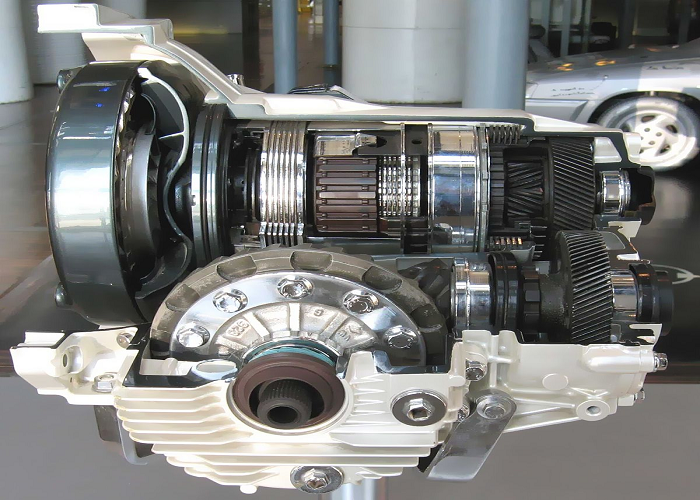
\includegraphics[width = 0.9\textwidth]{Figures/Cap2/Caixa_de_velocidades.png}
        \caption{}
        \label{fig:caixa_de_velocidades}
    \end{subfigure}%
    \begin{subfigure}{.5\textwidth}
        \centering
        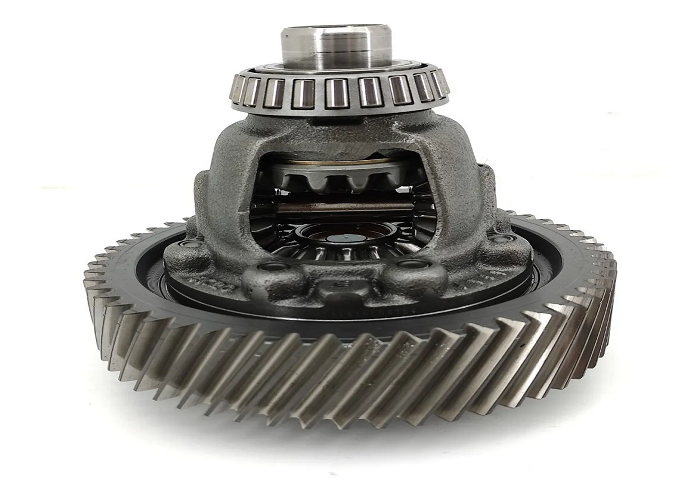
\includegraphics[width = 0.9\textwidth]{Figures/Cap2/Caixa_diferencial.png}
        \caption{}
        \label{fig:diferencial_montado}
    \end{subfigure}
\caption[Uma caixa de velocidades e uma caixa diferencial]%
{À esquerda, uma fotografia de uma caixa de velocidades JT4 aberta para ensaio. À direita, um veio diferencial DB45 com as engrenagens planetárias, antes de ser montada numa caixa de velocidades.}
\end{figure}
%%%%%%%%%%%%%%%%%%%%%%%%%%%%%%%%%%%%%%%%%%%%%%%%%%%%%%%%%%%%%%%%%%%%%%%%%%%%%
\newpage
\par
Uma engrenagem é um sistema mecânico que consiste em duas rodas dentadas que se interligam para transmitir o movimento entre elas. No âmbito deste trabalho, diretamente ligado à transmissão de movimento, as duas rodas dentadas transmitem potência por contacto mutuo da superfície dos dentes conjugados. Uma engrenagem é composta por um pinhão, a roda mais pequena, que pode estar associada a uma roda, uma cremalheira, uma coroa ou um parafuso sem-fim.
\par
Dos modos de solicitação nos dentes das engrenagens, os mais importantes são a flexão do dente devido ao momento fletor na base do dente gerado pela força de engrenamento e as tensões de Hertz, geradas pelo contacto mútuo entre flancos de dois dentes engrenados \cite{Completo2019}.
%%%%%%%%%%%%%%%%%%%%%%%%%%%%%%%%%%%%%%%%%%%%%%%%%%%%%%%%%%%%%%%%%%%%%%%%%%%%%
\begin{figure}[htb]
    \centering
    \begin{subfigure}{.5\textwidth}
        \centering
        \includegraphics[width = 0.9\textwidth]{Figures/Cap2/Completo_rodas.png}
        \caption{}
        \label{fig:dentes elicoidais}
    \end{subfigure}%
    \begin{subfigure}{.5\textwidth}
        \centering
        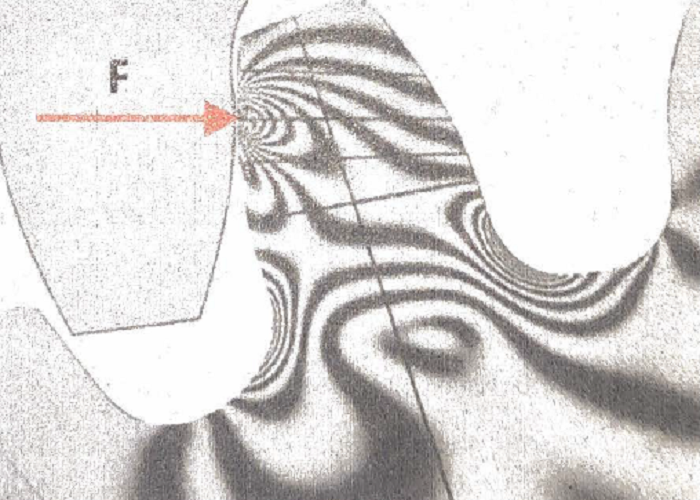
\includegraphics[width = 0.9\textwidth]{Figures/Cap2/Completo2019.png}
        \caption{}
        \label{fig:franjas_fotoelásticas}
    \end{subfigure}
\caption[Engrenagem de eixos paralelos e um padrão de franjas fotoelásticas]%
{À esquerda, uma engrenagem de eixos paralelos e dentes helicoidais.À direita, um padrão de franjas fotoelásticas referente ao gradiente de tensão de dentado reto.\cite{Completo2019}.}
\end{figure}
%%%%%%%%%%%%%%%%%%%%%%%%%%%%%%%%%%%%%%%%%%%%%%%%%%%%%%%%%%%%%%%%%%%%%%%%%%%%%
\par  
Enquanto a flexão do dente é tão maior quanto maior a sua tenacidade, a Resistência ao Contacto, pelas tensões de Hertz, segue o caminho oposto, sendo esta fortemente ligada à dureza. A tenacidade geralmente segue uma relação inversa com a dureza, portanto, um material muito duro, geralmente tem baixa tenacidade.
Dito isto, é então importante ser realizado um Tratamento na Superfície de Contacto entre a engrenagem, para lhe conferir uma maior dureza superficial sem interferir na capacidade do pé do dente de absorver energia de deformação, adquirindo às rodas dentadas bons coeficientes de resistência tanto em relação aos dois modos de solicitação. Além disso, é interessante que a superfície de contacto entre a roda dentada e o veio de transmissão de potência não sofra tratamento, sendo esta ‘interface’ estática, é idealmente pretendido uma maior tenacidade, pelo que é importante minimizar, nesta superfície, as ações sofridas pelo tratamento térmico realizado na roda dentada.
\newpage
%%%%%%%%%%%%%%%%%%%%%%%%%%%%%%%%%%%%%%%%%%%%%%%%%%%%%%%%%%%%%%%%%%%%%%%%%%%%%
\section{Tratamentos Térmicos} \label{sec:soa_tratamentos}
%%%%%%%%%%%%%%%%%%%%%%%%%%%%%%%%%%%%%%%%%%%%%%%%%%%%%%%%%%%%%%%%%%%%%%%%%%%%%
\subsection{Têmpera} \label{ssec:soa_tratamentos_tempera}

Têmpera é o arrefecimento rápido de uma peça metálica em água, óleo, polímero líquido, ou outros fluidos para obter determinadas propriedades dos materiais onde se visa evitar a ocorrência de processos como transformações de fase. Isto é possível ao imergir a peça metálica num fluido a baixa temperatura, aumentando rapidamente o gradiente de temperaturas entre a superfície da peça e o meio externo e diminuindo o tempo em que o material está às temperaturas favoráveis às transformações de fase\cite{Chaus2006}.O seu termo em inglês é “Quenching” e não deve ser confundido com “Tempering”, que em português traduz-se por Revenido.
%%%%%%%%%%%%%%%%%%%%%%%%%%%%%%%%%%%%%%%%%%%%%%%%%%%%%%%%%%%%%%%%%%%%%%%%%%%%%
\par
O mecanismo de obtenção de uma têmpera num aço, requer que seja atingida uma temperatura de austenitização, portanto, esta temperatura é intrínseca de cada liga(Ver Figura \ref{fig:Iron_Carbon_Diagram}). Geralmente, uma temperatura cerca de 50 \textdegree C acima da temperatura teórica é mantida durante algumas horas de forma a assegurar que há uma transformação total da microestrutura do aço da liga.
%%%%%%%%%%%%%%%%%%%%%%%%%%%%%%%%%%%%%%%%%%%%%%%%%%%%%%%%%%%%%%%%%%%%%%%%%%%%%
\begin{figure}[htb]
    \centering
    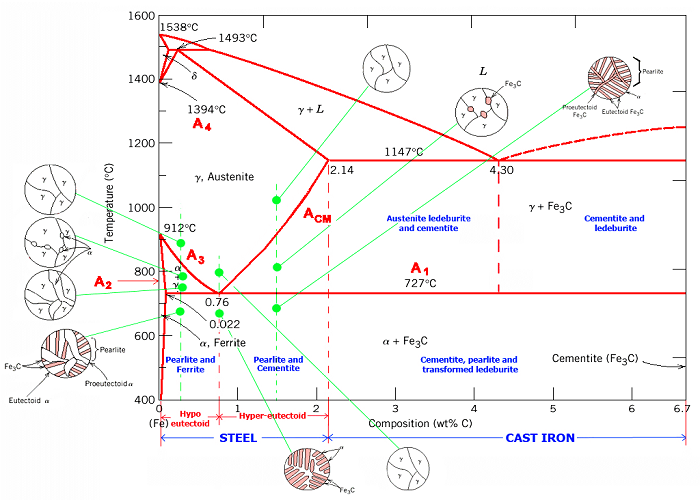
\includegraphics[width = 0.6\textwidth]{Figures/Cap2/Iron_Carbon_Diagram.png}
    \caption[Gráfico de fases do aço. Carbono x Ferro]%
    {Gráfico de fases do aço sem elementos de liga. Carbono x Ferro\cite{FollSD}. }
    \label{fig:Iron_Carbon_Diagram}
\end{figure}
%%%%%%%%%%%%%%%%%%%%%%%%%%%%%%%%%%%%%%%%%%%%%%%%%%%%%%%%%%%%%%%%%%%%%%%%%%%%%
\par
Uma vez que o aço tenha atingido a temperatura de austenitização, este é arrefecido rapidamente, de forma a evitar a etapa de transformação da microestrutura e impedindo a austenite de voltar ao estado de ferrite, estado de estabilidade da microestrutura do aço à temperatura ambiente. Uma vez que a obtenção da microestrutura final não seria possível sem o uso de um mecanismo como a têmpera, este tipo de microestrutura é chamada “microestrutura metastável”, e denomina-se martensite.
%%%%%%%%%%%%%%%%%%%%%%%%%%%%%%%%%%%%%%%%%%%%%%%%%%%%%%%%%%%%%%%%%%%%%%%%%%%%%
\par
Uma consequência da instabilidade da martensite, é que esta pode ser transformada noutros tipos de microestruturas mais estáveis, uma vez que se atinja uma temperatura que possibilite tal ocorrência. Uma das finalidades da têmpera, o aumento da dureza e da resistência, é obtido devido a esta alteração da microestrutura, uma vez que o tamanho dos grãos de martensite é menor que os grãos de ferrite, aumenta-se consequentemente a dureza\cite{Krauss2015}. Outro motivo para o aumento da dureza deve-se ao nível de tensões internas nos grãos de martensite é extremamente elevado, devido à natureza da disposição dos átomos nas duas microestruturas cristalinas. (Ver Figura \ref{fig:Crystal})
%%%%%%%%%%%%%%%%%%%%%%%%%%%%%%%%%%%%%%%%%%%%%%%%%%%%%%%%%%%%%%%%%%%%%%%%%%%%%
\begin{figure}[htb]
    \centering
    \begin{subfigure}{.5\textwidth}
      \centering
      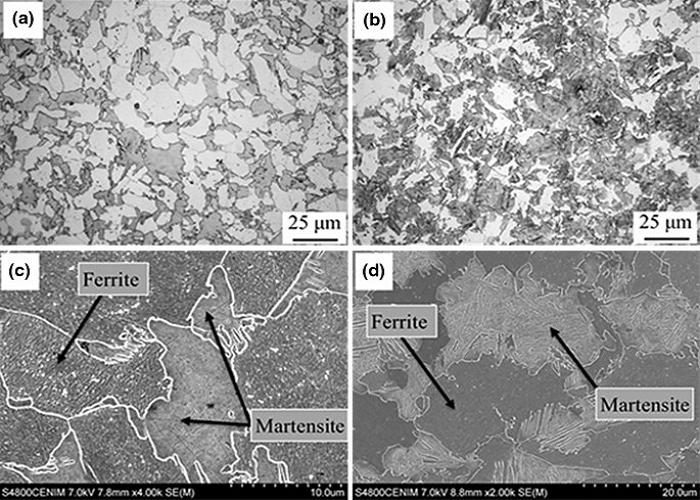
\includegraphics[width = 0.9\textwidth]{Figures/Cap2/Ferrite_Martensite.png}
      \caption{}
      \label{fig:Crystal}
    \end{subfigure}%
    \begin{subfigure}{.5\textwidth}
      \centering
      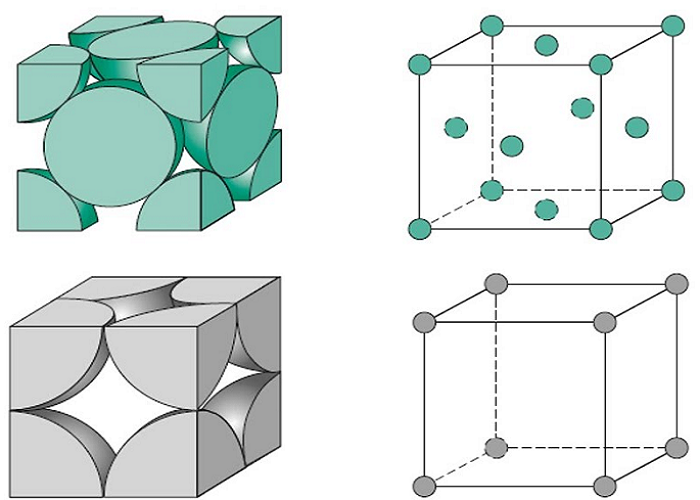
\includegraphics[width = 0.9\textwidth]{Figures/Cap2/CFC_CS.png}
      \caption{}
      \label{fig:CFC_CS}
    \end{subfigure}
\caption[Diferenças entre microestruturas de martensite e ferrite]%
{À esquerda, uma imagem microscópica dos grãos de ferrite e martensite, respetivamente indicados por meio de setas nas figuras. À direita, respetivamente de cima para baixo, a estrutura cristalina CFC da martensite, e a estrutura cristalina CS da ferrite.}
\end{figure}
%%%%%%%%%%%%%%%%%%%%%%%%%%%%%%%%%%%%%%%%%%%%%%%%%%%%%%%%%%%%%%%%%%%%%%%%%%%%%
\par
Outra razão para o aumento da dureza e da resistência, é que a martensite tem uma estrutura cúbica de face centrada(Ver Figura \ref{fig:CFC_CS}), ao contrário da ferrite, que é cúbica simples, sendo assim limitada nos graus de liberdade disponíveis sob os quais os átomos podem deslocar-se de uma estrutura cristalina para outra.
%%%%%%%%%%%%%%%%%%%%%%%%%%%%%%%%%%%%%%%%%%%%%%%%%%%%%%%%%%%%%%%%%%%%%%%%%%%%%
%%%%%%%%%%%%%%%%%%%%%%%%%%%%%%%%%%%%%%%%%%%%%%%%%%%%%%%%%%%%%%%%%%%%%%%%%%%%%
\begin{figure}[htb]
    \centering
    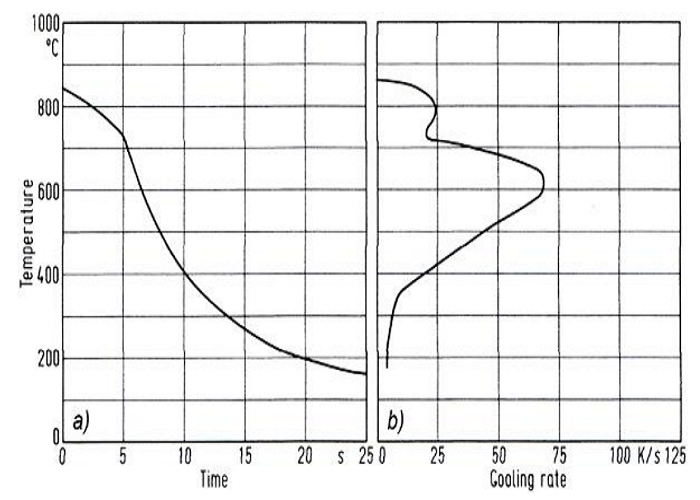
\includegraphics[width = 0.6\textwidth]{Figures/Cap2/Tempera_Arrefecimento.png}
    \caption[Curva de arrefecimento em fluido de têmpera]%
    {Curvas de arrefecimento de uma peça imersa num fluido de têmpera.}
    \label{fig:tempera_arref}
\end{figure}
%%%%%%%%%%%%%%%%%%%%%%%%%%%%%%%%%%%%%%%%%%%%%%%%%%%%%%%%%%%%%%%%%%%%%%%%%%%%%
\par
No entanto, a microestrutura resultante e as propriedades mecânicas associadas dependem da taxa de arrefecimento obtida durante o processo de têmpera. Na curva de arrefecimento da Figura \ref{fig:tempera_arref}, podem ser verificadas três fases de arrefecimento. A primeira consiste no arrefecimento por meio de uma camada de vapor, onde a maior parte do calor é transferida por radiação. Esta camada é formada por um fenómeno chamado \textbf{“Efeito Leidenfrost”}, que ocorre quando um líquido entra em contacto com uma superfície significativamente mais quente do que seu ponto de ebulição. 
\newpage
\par
Nesse caso, uma camada de vapor é formada entre a superfície e o líquido, o que cria um isolamento térmico que impede a evaporação completa do líquido. Isso faz com que este “flutue” sobre a superfície, criando uma barreira de vapor que reduz a transferência de calor entre a superfície e o líquido. A segunda fase, que conta com a convecção como maior meio de transporte de calor, consiste no arrefecimento por transporte de vapor. Como já não se verifica a ocorrência do efeito Leidenfrost, é possível uma livre evaporação do fluido de têmpera, o que aumenta a velocidade de convecção, e por consequência, a velocidade de arrefecimento. A última fase, no entanto, dá-se quando a superfície já se encontra numa temperatura abaixo da temperatura de transformação de fase liquido-vapor do fluido, portanto a velocidade relativa do líquido é muito mais baixa que na segunda fase, e por consequência, a velocidade de arrefecimento significativamente mais baixa.

%%%%%%%%%%%%%%%%%%%%%%%%%%%%%%%%%%%%%%%%%%%%%%%%%%%%%%%%%%%%%%%%%%%%%%%%%%%%%
\subsection{Revenido} \label{ssec:soa_tratamentos_revenido}

O Revenido é um tipo de tratamento térmico normalmente utilizado após tratamento de Tempera que consiste em aquecer e manter o material até uma certa temperatura, abaixo da temperatura crítica, para então resfriar-se ao ar, e desta forma aliviar tensões residuais, diminuir dureza e aumentar tenacidade\cite{Krauss2015}. A combinação de um Revenido a seguir de uma Tempera também é conhecida como “Q\&T Treatment”.
%%%%%%%%%%%%%%%%%%%%%%%%%%%%%%%%%%%%%%%%%%%%%%%%%%%%%%%%%%%%%%%%%%%%%%%%%%%%%
\par
Aços tratados termicamente formam microestruturas martensíticas, que tem maior dureza, força, resistência à fadiga e desgaste resistência quando comparadas a microestruturas de ferrite, no entanto, estruturas martensíticas obtidas por têmpera tem baixa resistência à fratura e tenacidade\cite{Krauss2001}. Uma vez que o tratamento de aços com microestruturas martensíticas são tradicionalmente monitorados por medições de dureza, é importante demonstrar que existe uma relação entre a temperatura do revenido, a quantidade de carbono do aço e a sua dureza final(Ver \textbf{Figura}\ref{fig:Hardness_Temperature_Carbon}). Consequentemente, a quantidade de microestruturas martensíticas e a resistência à fratura e tenacidade do aço que sobre o revenido depende da temperatura do processo.
\par
Tipicamente, as temperaturas de revenido rondam os (150 – 400) \textdegree C, onde o objetivo é reter a maioria das estruturas martensíticas. Em geral, qualquer temperatura pode ser utilizada ao se realizar um revenido, no entanto, as temperaturas mais utilizadas normalmente conferem boa relação entre as propriedades adquiridas pela tempera, sem abdicar da resistência à fratura e tenacidade do material.
%%%%%%%%%%%%%%%%%%%%%%%%%%%%%%%%%%%%%%%%%%%%%%%%%%%%%%%%%%%%%%%%%%%%%%%%%%%%%
\begin{figure}[htb]
    \centering
    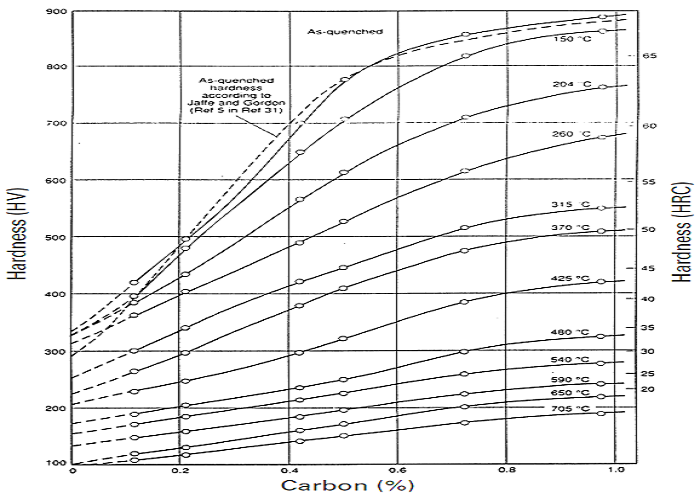
\includegraphics[width = 0.6\textwidth]{Figures/Cap2/Hardness_Temperature_Carbon.png}
    \caption[Relação Revenido: Dureza x Temperatura]%
    {Relação entre temperatura, quantidade de carbono e a dureza de um aço após um revenido\cite{Krauss2001}.}
    \label{fig:Hardness_Temperature_Carbon}
\end{figure}
%%%%%%%%%%%%%%%%%%%%%%%%%%%%%%%%%%%%%%%%%%%%%%%%%%%%%%%%%%%%%%%%%%%%%%%%%%%%%
\subsection{Cementação} \label{ssec:soa_tratamentos_cementação}

Cementação ou carburação é um tratamento termoquímico que consiste em se introduzir carbono na superfície do aço, o que pode ser feito por meio de uma atmosfera controlada, rica em carbono, visando-se aumentar a dureza superficial do material. O mecanismo de ação da cementação é idêntico ao da carbonitruração, que será abordado na \textbf{\ref{ssec:soa_tratamentos_carbonitruracao}}. Com este tipo de tratamento, é possível aumentar superficialmente a percentagem de carbono no aço, aumentando a quantidade de microestrutura martensítica, consequentemente aumentando a dureza desta superfície, com interferências marginais no núcleo da peça tratada \cite{Oberg1989}.

%%%%%%%%%%%%%%%%%%%%%%%%%%%%%%%%%%%%%%%%%%%%%%%%%%%%%%%%%%%%%%%%%%%%%%%%%%%%%
\subsection{Nitruração}

De forma análoga à \textbf{Cementação}, a Nitruração é um tratamento termoquímico que visa a introdução de Azoto na superfície do aço. Também pode ser feita por meio de uma atmosfera controlada. O objetivo da introdução do azoto é criar uma distorção na rede cristalina da microestrutura de forma a aumentar a dureza e modificar outras características do material, superficialmente. Um estudo da microestrutura, feito por meio da utilização da espectroscopia de energia dispersiva (EDS, em ingles “Energy Dispersive Spectroscopy”), em raios-x mostra a composição da camada de tratamento térmico, numa região de dimensões (112 × 140) $\mu$ m junto à borda do material, onde a superfície tratada tem aproximadamente (40 – 45) $\mu$m de comprimento onde é maioritariamente composta por ligas de ferro-azoto, que por no que lhe concerne, até o comprimento de (20 – 25) $\mu$ m, é maioritariamente composta por Fe\textsubscript{3}N \cite{EDAX2023}, como pode ser visto na Figura \ref{fig:Nitriding_3_microstructure}.
%%%%%%%%%%%%%%%%%%%%%%%%%%%%%%%%%%%%%%%%%%%%%%%%%%%%%%%%%%%%%%%%%%%%%%%%%%%%%
\begin{figure}[htb]
    \centering
    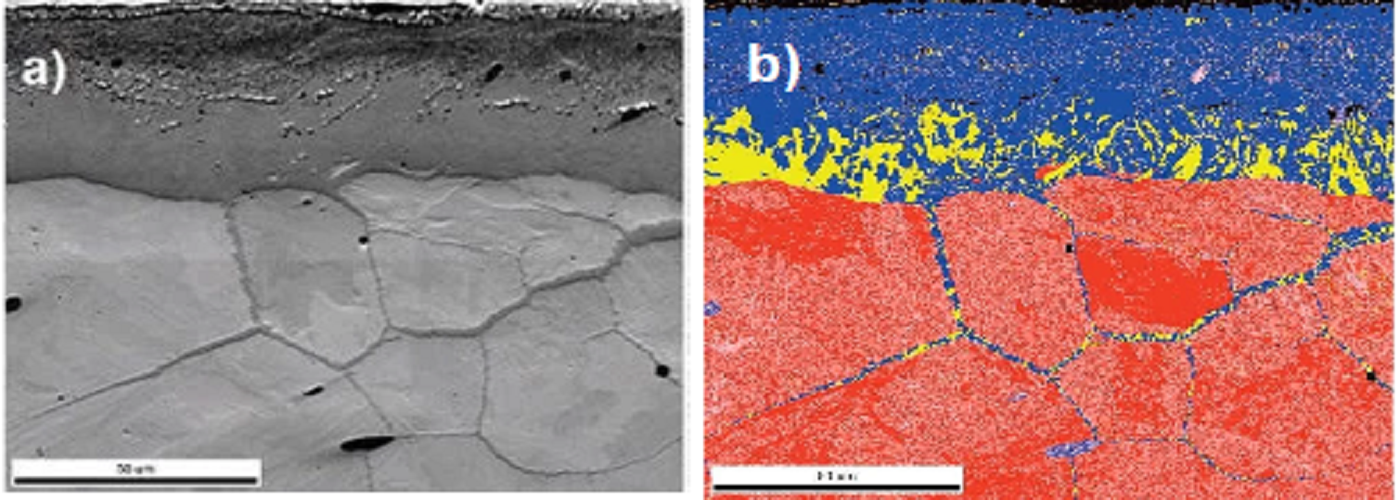
\includegraphics[width = 0.9\textwidth]{Figures/Cap2/Nitriding_3_microstructure.png}
    \caption[Microestruturas de uma peça tratada por nitruração]%
    {Imagens mostrando diferentes contrastes microestruturais na proximidade da superfície da peça tratada\cite{EDAX2023}, e o mapa de fases recolhido com as diversas microestruturas. Em vermelho, ferrite; em azul, Fe\textsubscript{4}N; em amarelo Fe\textsubscript{3}N; e em cor-de-rosa, MnS\textsubscript{2}.}
    \label{fig:Nitriding_3_microstructure}
\end{figure}
%%%%%%%%%%%%%%%%%%%%%%%%%%%%%%%%%%%%%%%%%%%%%%%%%%%%%%%%%%%%%%%%%%%%%%%%%%%%%
\newpage
\par
Outro estudo investigou a influência do tempo de tratamento, a temperatura e o volume de azoto na atmosfera da nitruração de um aço de baixa liga AISI 5140, equivalente ao DIN 41Cr4, e definiu a gama de temperaturas em cerca de (450 – 550)°C para um tempo de tratamento de 1 a 12 horas\cite{Karaoglu2002}. A lista de tempos e temperaturas pode ser vista na \textbf{Tabela} \ref{tab:Nitriding_cond}. Os resultados obtidos podem ser vistos na \textbf{Figura} \ref{fig:Nitriding_gradients}.
%%%%%%%%%%%%%%%%%%%%%%%%%%%%%%%%%%%%%%%%%%%%%%%%%%%%%%%%%%%%%%%%%%%%%%%%%%%%%
\begin{table}[htb]
    \centering
    \caption[Condições dos testes das amostras com vários parâmetros de nitruração]%
    {Condições dos testes dos grupos de amostras\cite{Karaoglu2002}.}
    \label{tab:Nitriding_cond}
    \begin{tabular}{cccc} 
    \toprule
    \textbf{Grupo de amostras} & \textbf{Tempo (h)} & \textbf{Temperatura (°C)} & \textbf{Azoto (vol.\%)}  \\ 
    \hline\hline
    1.500.20                   & 1                  & 500                       & 20                       \\
    4.500.20                   & 4                  & 500                       & 20                       \\
    12.500.20                  & 12                 & 500                       & 20                       \\
    4.450.20                   & 4                  & 450                       & 20                       \\
    4.550.20                   & 4                  & 550                       & 20                       \\
    4.500.60                   & 4                  & 500                       & 60                       \\
    \bottomrule
    \end{tabular}
\end{table}
%%%%%%%%%%%%%%%%%%%%%%%%%%%%%%%%%%%%%%%%%%%%%%%%%%%%%%%%%%%%%%%%%%%%%%%%%%%%%
\begin{figure}[htb]
    \centering
    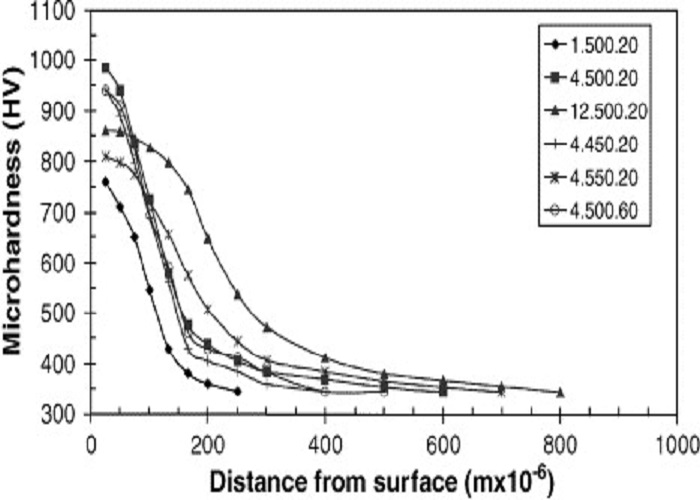
\includegraphics[width = 0.6\textwidth]{Figures/Cap2/Nitriding_gradients.jpg}
    \caption[Durezas obtidas após nitruração]%
    {Valores das durezas obtidas das várias amostras de AISI 5140, para os vários valores de tempo, temperatura e composição da atmosfera\cite{Karaoglu2002}.}
    \label{fig:Nitriding_gradients}
\end{figure}
%%%%%%%%%%%%%%%%%%%%%%%%%%%%%%%%%%%%%%%%%%%%%%%%%%%%%%%%%%%%%%%%%%%%%%%%%%%%%
\par
Destes resultados, é possível identificar uma correlação direta, nesta liga, entre o tempo de carbonitruração e a profundidade da camada tratada, uma vez que para temperaturas e atmosferas semelhantes, o grupo de amostras 1.500.20, com tempo de tratamento de 1 hora, tem dureza a 100 $\mu$ m da superfície de cerca de 550 HV, enquanto o grupo 12.500.20, tem dureza a 100 $\mu$m de cerca de 825 HV. No entanto, as temperaturas, desde que dentro do intervalo estudado, mostram-se pouco relevantes, uma vez que os valores de dureza das amostras com 4 horas de tratamento e 20\% de volume de azoto tem curvas de tensão x profundidade muito semelhantes.
%%%%%%%%%%%%%%%%%%%%%%%%%%%%%%%%%%%%%%%%%%%%%%%%%%%%%%%%%%%%%%%%%%%%%%%%%%%%%
\newpage
\subsection{Carbonitruração} \label{ssec:soa_tratamentos_carbonitruracao}

A carbonitruração, no que lhe concerne, é um processo cujo objetivo é muito semelhante ao da \textbf{Cementação}, e que se diferencia deste uma vez que é adicionado amoníaco (NH\textsubscript{3}) de forma a adicionar azoto à superfície tratada, de forma a melhorar a temperabilidade e possibilitar a formação de martensite em aços de carbono e de baixa liga que inicialmente têm baixa temperabilidade\cite{Herring2011}. Uma das principais vantagens da carbonitruração relativamente à cementação, é que o processo é relativamente mais rápido, conformando uma menor espessura de tratamento, e facilitando a formação de martensite em aços de baixa liga, tornando-o uma escolha altamente rentável para uma vasta gama de aplicações.
Como a cementação, é um processo de tratamento térmico de endurecimento superficial utilizado para melhorar a dureza, resistência ao desgaste e resistência à fadiga de ligas de aço, e ferro fundido, que por sua vez, envolve a difusão de carbono e azoto na superfície do material para formar uma fina camada superficial dura e resistente ao desgaste, enquanto o núcleo do material é mantido dúctil, proporcionando melhores propriedades de superfície, propriedades estas, ideais para a aplicação em questão, uma vez que a coroa é um componente mecânico sujeito a elevados níveis de tensões e desgaste\cite{Bryson2009}. Um exemplo da microestrutura de um aço de baixa liga tratado por carbonitruração pode ser visto na figura \ref{fig:Carbonitriding_microstructure}.
%%%%%%%%%%%%%%%%%%%%%%%%%%%%%%%%%%%%%%%%%%%%%%%%%%%%%%%%%%%%%%%%%%%%%%%%%%%%%
\begin{figure}[htb]
    \centering
    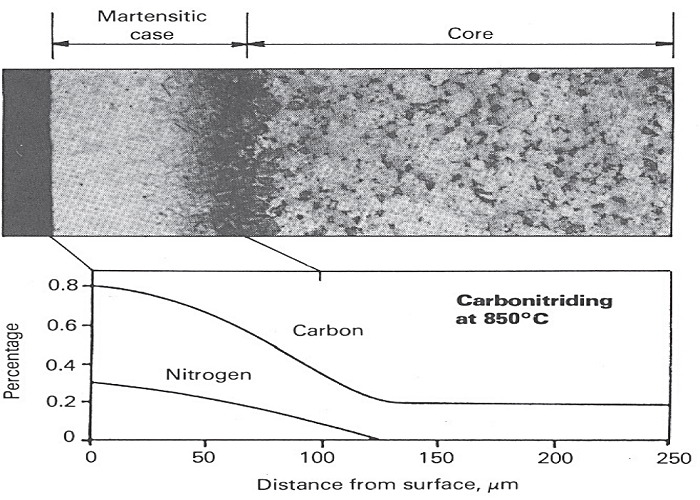
\includegraphics[width = 0.6\textwidth]{Figures/Cap2/Carbonitriding_microstructure.png}
    \caption[Micrografia de uma peça tratada por carbonitruração]%
    {Micrografia das camadas superficiais produzidas por carbonitruração de um aço a 850 \textdegree C. Pode-se observar uma camada martensítica no exterior, e um núcleo predominantemente formado por ferrite\cite{Herring2011}.}
    \label{fig:Carbonitriding_microstructure}
\end{figure}
%%%%%%%%%%%%%%%%%%%%%%%%%%%%%%%%%%%%%%%%%%%%%%%%%%%%%%%%%%%%%%%%%%%%%%%%%%%%
\par
O processo de carbonitruração é realizado ao se aquecer a peça a ser tratada numa atmosfera controlada até uma temperatura por volta de (700 – 900) \textdegree C, num forno de atmosfera controlada que contém Amoníaco (NH\textsubscript{3}) e alguma fonte de Carbono, como, por exemplo, propano (C\textsubscript{3}H\textsubscript{8}), de forma a causar a difusão de carbono e azoto na superfície do metal, formando uma camada que tem tipicamente de 0,5 a 1,5 milímetros de espessura\cite{Rajan2011}, sendo esta profundidade da superfície tratada dependente das condições do processo, incluindo a temperatura, o tempo e a composição da atmosfera. A Figura \ref{fig:Carbonitriding_depth} exemplifica graficamente a dependência entre a profundidade, a temperatura e o tempo.
%%%%%%%%%%%%%%%%%%%%%%%%%%%%%%%%%%%%%%%%%%%%%%%%%%%%%%%%%%%%%%%%%%%%%%%%%%%%
\begin{figure}[htb]
    \centering
    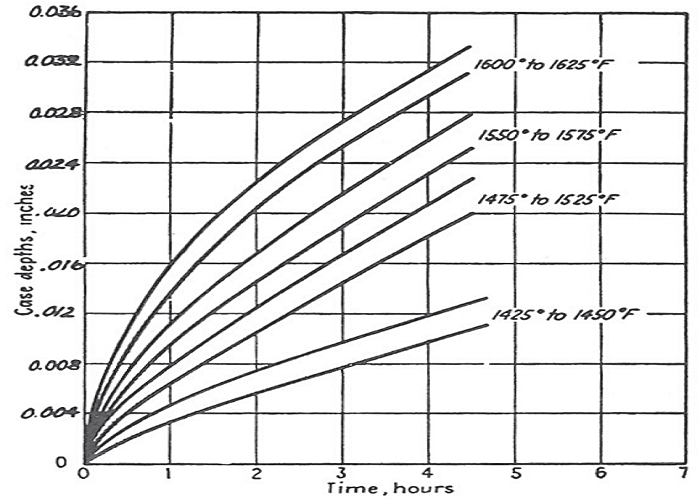
\includegraphics[width = 0.6\textwidth]{Figures/Cap2/Carbonitriding_depth.png}
    \caption[Composição de carbono e azoto em relação à profundidade de tratamento]%
    {Gráfico que mostra a profundidade do tratamento de carbonitruração, em polegadas relativamente ao tempo de tratamento, em horas, para várias temperaturas, em Fahrenheit.\cite{Herring2011}}
    \label{fig:Carbonitriding_depth}
\end{figure}%%%%%%%%%%%%%%%%%%%%%%%%%%%%%%%%%%%%%%%%%%%%%%%%%%%%%%%%%%%%%%%%%%%%%%%%%%%%%
\newpage
\par
Outra correlação importante em peças tratadas por carbonitruração, é a correlação entre a dureza e a taxa percentual de carbono, sendo estas quase diretamente relacionadas, pelo que, uma vez que a dureza da camada é mais baixa, pode-se assumir que a taxa de carbono no ponto também o é, evitando assim que uma análise da micrografia do material, a qual é um ensaio destrutivo, seja feita sempre que se queira verificar a quantidade de carbono depositado no ponto em questão. Esta correlação pode ser visualizada na figura \ref{fig:Carbon_Hardness_Carbonitriding}
%%%%%%%%%%%%%%%%%%%%%%%%%%%%%%%%%%%%%%%%%%%%%%%%%%%%%%%%%%%%%%%%%%%%%%%%%%%%%
\begin{figure}[htb]
    \centering
    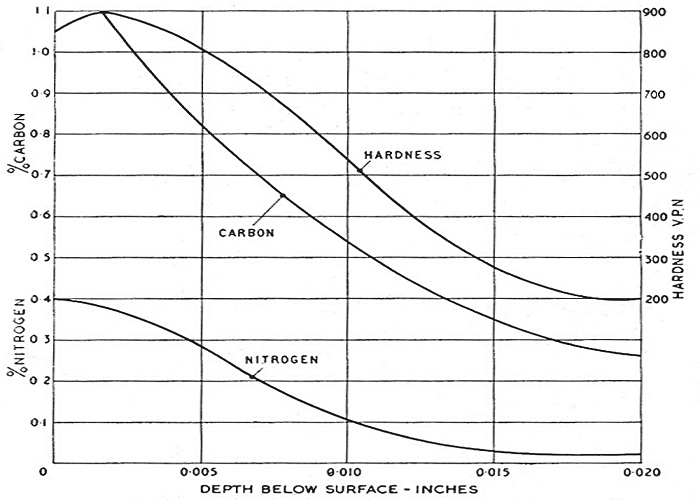
\includegraphics[width = 0.6\textwidth]{Figures/Cap2/Carbon_Hardness_Carbonitriding.png}
    \caption[Relação entre carbono, azoto e dureza]%
    {Gráfico que mostra a relação entre a quantidade de carbono no ponto e a dureza\cite{Herring2011}. Mais uma vez, pode-se observar que a deposição de carbono diminui à medida que a distância da superfície tratada aumenta.}
    \label{fig:Carbon_Hardness_Carbonitriding}
\end{figure}
%%%%%%%%%%%%%%%%%%%%%%%%%%%%%%%%%%%%%%%%%%%%%%%%%%%%%%%%%%%%%%%%%%%%%%%%%%%%%
\newpage
\par
Por fim, a têmpera é um passo essencial após a carbonitruração, uma vez que ajuda a solidificar as posições dos átomos de carbono e azoto adquiridos na etapa da carbonitruração, formando as estruturas martensíticas discutidas no Subcapítulo \ref{ssec:soa_tratamentos_tempera}. Sem uma têmpera, o aço pode não atingir a dureza e resistência desejadas. Evidentemente, uma vez que a superfície que sofreu a carbonitruração tem uma composição de carbono superior à composição do núcleo, esta superfície deve tornar-se mais dura que o núcleo, mas será maioritariamente composta por ferrite, que, ao contrário da martensite, não confere uma dureza tão elevada ao material. É importante evidenciar que, mesmo que não seja feita uma têmpera, o aço tratado ainda poderá ter elevados níveis de deformações originadas pela energia térmica obtida na etapa de adsorção de carbono e azoto, porquanto a superfície tem uma composição química ligeiramente diferente do núcleo, o que pode ocasionar diferentes gradientes de temperatura e diferentes deslocamentos. Por conseguinte, é essencial que sejam seguidas as etapas adequadas do tratamento térmico, para serem alcançadas as propriedades desejadas e assegurar a obtenção do produto final.
%%%%%%%%%%%%%%%%%%%%%%%%%%%%%%%%%%%%%%%%%%%%%%%%%%%%%%%%%%%%%%%%%%%%%%%%%%%%%
\section{Soldadura}\label{sec:soldadura}
%%%%%%%%%%%%%%%%%%%%%%%%%%%%%%%%%%%%%%%%%%%%%%%%%%%%%%%%%%%%%%%%%%%%%%%%%%%%%
\subsection{Soldabilidade de aços-carbono}\label{ssec:soldadura-soldabilidade}

A soldadura de metais e ligas é um processo crucial na confeção de caixas de velocidade. No entanto, a soldabilidade de diferentes ligas pode ser afetada pelo percentual de  \textbf{carbono equivalente} — em inglês “Carbon Equivalent”, ou CE — da liga, a qual é uma medida da soldabilidade de uma liga que tem em conta não só a percentagem de carbono como também outros elementos de liga. Existe alguma investigação sobre o impacto da CEP na soldabilidade, reiterando a importância de controlar a quantidade de carbono nas zonas onde serão realizados processos de soldadura.
\par
A Equação \ref{eq:CE-IIW}, foi desenvolvida por Dearden and O'Neill e adotada pelo Instituto Internacional de Soldadura em 1967, sendo considerada adequada para prever a temperabilidade numa grande variedade de aços de carbono simples e aços carbono-manganês, mas não para aços microligados de alta resistência de baixa liga ou aços de baixa liga CrMo. Esta fórmula considera os efeitos combinados do carbono e de outros elementos de liga sobre a temperabilidade do aço. O valor do CE é expresso como uma percentagem, onde os valores de referência em relação à soldabilidade é descrita na Tabela \ref{tab:CE}.
\vspace{5mm}
%%%%%%%%%%%%%%%%%%%%%%%%%%%%%%%%%%%%%%%%%%%%%%%%%%%%%%%%%%%%%%%%%%%%%%%%%%%%%
\begin{equation}
    \centering
    \label{eq:CE-IIW}
    \%C + \frac{\%Mn}{6}+\frac{\%Cr+\%Mo+\%V}{5}+\frac{\%Cu+\%Ni}{15}
\end{equation}
%%%%%%%%%%%%%%%%%%%%%%%%%%%%%%%%%%%%%%%%%%%%%%%%%%%%%%%%%%%%%%%%%%%%%%%%%%%%%
\vspace{5mm}
\par
O cálculo do CE envolve a adição das percentagens de peso dos vários elementos de liga no aço, sendo cada elemento multiplicado por um fator específico. O total resultante é então adicionado à percentagem de carbono da liga, obtendo-se assim, o valor do percentual CE da liga.
\par
Um percentual de CE mais elevado pode levar a questões como o aumento da porosidade, rachadura, e redução da tenacidade na ZAT (Zona Afetada Termicamente)\cite{Karsamas2003} e um aumento de austenite retida\cite{Park2018}, o que leva ao aumento das tensões internas do material, e pode comprometer a resistência e integridade da estrutura soldada.
\par
Para além do seu impacto na qualidade da soldadura, existe uma relação entre o percentual de  CE e a geometria do cordão de solda em aços com baixo teor de carbono. Um percentual de CE mais elevado leva a formas mais irregulares do granulo e a uma maior probabilidade de “undercutting” — termo utilizado para quando a solda reduz a espessura da secção transversal do metal de base, reduzindo a resistência da soldadura e das peças de trabalho — que podem ser difíceis de reparar e podem aumentar o tempo e os custos de produção.
%%%%%%%%%%%%%%%%%%%%%%%%%%%%%%%%%%%%%%%%%%%%%%%%%%%%%%%%%%%%%%%%%%%%%%%%%%%%%
\begin{table}[htb]
    \centering
    \caption[Valores de referência para a soldabilidade de percentuais CE]%
    {Valores de referência para a soldabilidade de percentuais CE \cite{Vladimir2000}.}
    \label{tab:CE}
    \begin{tabular}{cc} 
    \toprule
    CE              & Soldabilidade  \\ 
    \hline\hline
    0.00\% — 0.35\% & Excelente      \\
    0.36\% — 0.40\% & Ótima          \\
    0.41\% — 0.45\% & Boa            \\
    0.46\% — 0.49\% & Razoável       \\
    0.50\% ou maior & Má             \\
    \bottomrule
    \end{tabular}
\end{table}
%%%%%%%%%%%%%%%%%%%%%%%%%%%%%%%%%%%%%%%%%%%%%%%%%%%%%%%%%%%%%%%%%%%%%%%%%%%%%
\subsection{Fissuração induzida por hidrogénio}\label{ssec:soldadura-fissuracao}

A fissuração induzida pelo hidrogénio é um tipo de corrosão que ocorre em componentes metálicos quando estes são expostos a um ambiente rico em hidrogénio, que ocorre quando há migração de hidrogénio do meio para o metal, que pode ocorrer por fontes externas, tais como proteção catódica ou corrosão assistida por hidrogénio, ou por fontes internas, tais como captação de hidrogénio durante a soldadura. Uma vez dentro do metal, o hidrogénio pode causar uma acumulação de pressão interna, levando à formação de fissuras que podem então propagar-se rapidamente, resultando numa falha completa do componente. Uma vez que a atmosfera no forno para a carbonitruração tem como os seus principais constituintes, o amoníaco (NH\textsubscript{3}) e monóxido de carbono (CO), e sendo a temperatura de dissociação do amoníaco por volta de 500\textdegree C, torna a atmosfera, também, rica em hidrogénio.
%%%%%%%%%%%%%%%%%%%%%%%%%%%%%%%%%%%%%%%%%%%%%%%%%%%%%%%%%%%%%%%%%%%%%%%%%%%%%
\begin{figure}[htb]
    \centering
    \begin{subfigure}{.4\textwidth}
        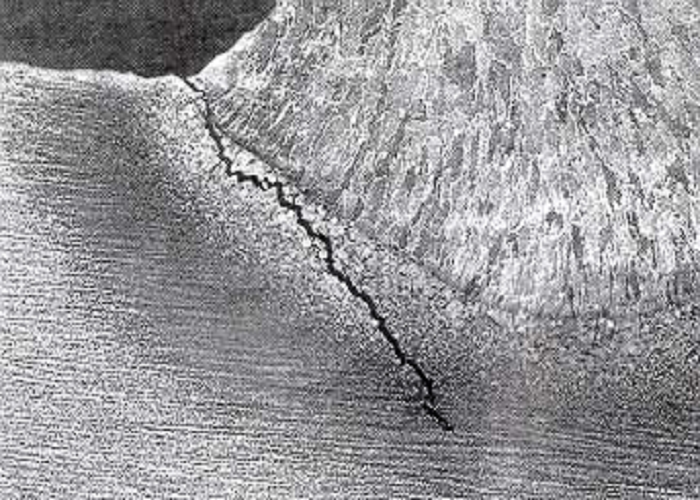
\includegraphics[width = 0.9\textwidth]{Figures/Cap2/Cold_Cracking.png}
        \caption{}
        \label{fig:Fissuracao_1}
    \end{subfigure}%
    \begin{subfigure}{.4\textwidth}
        \centering
        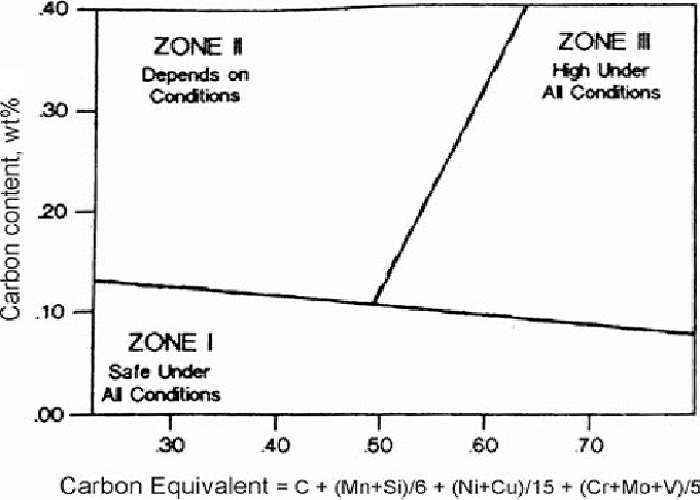
\includegraphics[width = 0.9\textwidth]{Figures/Cap2/Graville_Diagram.png}
        \caption{}
        \label{fig:Graville}
    \end{subfigure}
    \caption[Fissuração induzida por hidrogénio e correlação de Graville]%
    {À esquerda, uma fissuração induzida pelo hidrogénio presente na ZAT (Zona Afetada Termicamente) de uma peça soldada. À direita, correlação de Graville, que correlaciona o percentual de carbono e o percentual de carbono equivalente com ocorrência de fissuras na ZAT (Zona afetada termicamente)\cite{Olson2007}. }
\end{figure}
%%%%%%%%%%%%%%%%%%%%%%%%%%%%%%%%%%%%%%%%%%%%%%%%%%%%%%%%%%%%%%%%%%%%%%%%%%%%%
%%%%%%%%%%%%%%%%%%%%%%%%%%%%%%%%%%%%%%%%%%%%%%%%%%%%%%%%%%%%%%%%%%%%%%%%%%%%%
\begin{figure}[htb]
    \centering
    \begin{subfigure}{.4\textwidth}
      \centering
      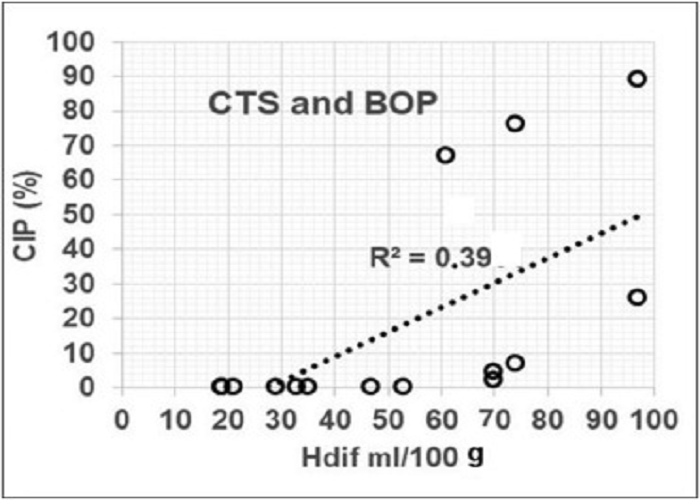
\includegraphics[width = 0.9\linewidth]{Figures/Cap2/Hdif_CE.png}
      \caption{}
      \label{fig:Hdif_CE}
    \end{subfigure}%
    \begin{subfigure}{.4\textwidth}
      \centering
      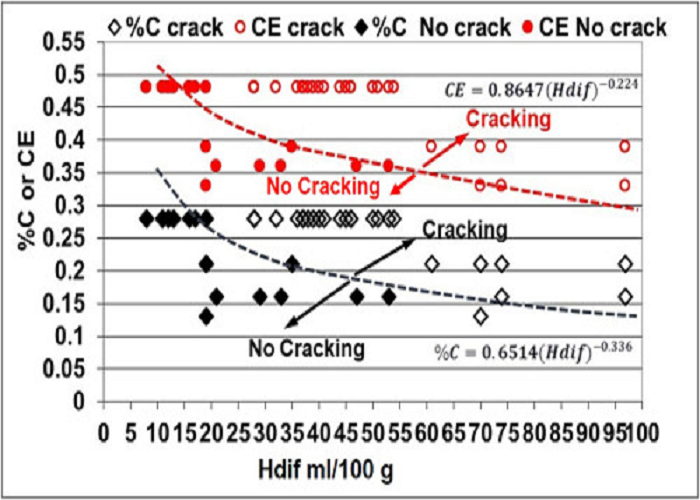
\includegraphics[width = 0.9\linewidth]{Figures/Cap2/CE_Hdif_Crack.png}
      \caption{}
      \label{fig:CE_Hdif_Crack}
    \end{subfigure}
    \caption[Correlações entre hidrogénio difusível e fissuração induzida por hidrogénio]%
    {À esquerda, uma correlação entre o hidrogénio difusível e a ocorrência de fissuração. À direita, uma correlação entre a fissuração a frio, o percentual de carbono ou a taxa CE, e o hidrogénio difusível.}
    \end{figure}
    %%%%%%%%%%%%%%%%%%%%%%%%%%%%%%%%%%%%%%%%%%%%%%%%%%%%%%%%%%%%%%%%%%%%%%%%%%%%%
\newpage
\par
Existe também uma correlação entre o tamanho dos grãos e a facilidade da ocorrência de fissuração\cite{Seo2008}, bem como a quantidade de inclusões não metálicas, como, por exemplo, o Azoto adicionado pelo processo de carbonitruração, isto é, quanto maior o tamanho dos grãos, ou seja, quanto menos espaço houver para a adsorção do hidrogénio, menor é a possibilidade da ocorrência do processo.
\par
De maneira análoga, quanto maior a quantidade de inclusões não metálicas, mais espaço há para a adsorção do hidrogénio, aumentando a possibilidade da ocorrência da fissuração. Um estudo verificou uma correlação entre a quantidade de hidrogénio difusível e a ocorrência de fissuração induzida por hidrogénio\cite{Santos2021} (Ver Figura \ref{fig:Hdif_CE}) em contentores soldados por arco submerso, bem como uma correlação entre a taxa percentual de carbono equivalente, a quantidade de hidrogénio difusível, e a ocorrência de fissuras (Ver Figura \ref{fig:CE_Hdif_Crack}). Com isto, desde que seja possível mensurar a quantidade de hidrogénio difusível, é possível estimar a probabilidade da ocorrência de uma fissura no material.
\par
Para além da relação entre o hidrogénio difusível e a ocorrência de fissuração, existe uma correlação entre o percentual de carbono e de carbono equivalente, denominada “Correlação de Graville”, que correlaciona estes dois valores com a ocorrência de fissuração da ZAT (Zona Afetada Termicamente) (Ver \textbf{Figura} \ref{fig:Graville})\cite{Olson2007}.

%%%%%%%%%%%%%%%%%%%%%%%%%%%%%%%%%%%%%%%%%%%%%%%%%%%%%%%%%%%%%%%%%%%%%%%%%%%%%
\par
Apesar de ainda não existir um mecanismo universalmente aceite para sua deteção, a fissuração por hidrogénio pôde ser correlacionada, nesta aplicação, com duas variáveis que podem ser facilmente medidas ou calculadas. Ainda que o hidrogénio seja muito difícil de detetar no estudo da microestrutura, existem ferramentas que permitem estimar a ocorrência de fissuração por hidrogénio.
%%%%%%%%%%%%%%%%%%%%%%%%%%%%%%%%%%%%%%%%%%%%%%%%%%%%%%%%%%%%%%%%%%%%%%%%%%%%%
\newpage
\subsection{Diagramas da curva de arrefecimento continuo}\label{ssec:diagramas_CCT}
Por fim, é importante mencionar os diagramas CCT (Continuous Cooling Transformation), ou diagramas de curva de arrefecimento contínuo. Estes diagramas mostram as transformações de fase que ocorrem em um material à medida que ele é arrefecido continuamente a partir da temperatura de austenitização e são utilizados para tentar prever as fases que serão formadas de acordo com a velocidade de arrefecimento a que o material for submetido.
\par
As curvas de arrefecimento contínuo são obtidas por meio de ensaios onde o arrefecimento é controlado, onde uma amostra do material é aquecida até a temperatura de austenitização e arrefecida a uma taxa constante. Dependendo da composição química do material, diferentes taxas de arrefecimento podem dar origem a diferentes estruturas finais. A taxa de arrefecimento e a temperatura onde ocorrem as transformações da microestruturas são representadas por meio de curvas, como pode ser visto na Figura \ref{fig:CCT_SOA}.
%%%%%%%%%%%%%%%%%%%%%%%%%%%%%%%%%%%%%%%%%%%%%%%%%%%%%%%%%%%%%%%%%%%%%%%%%%%%%
\begin{figure}[htb]
    \centering
    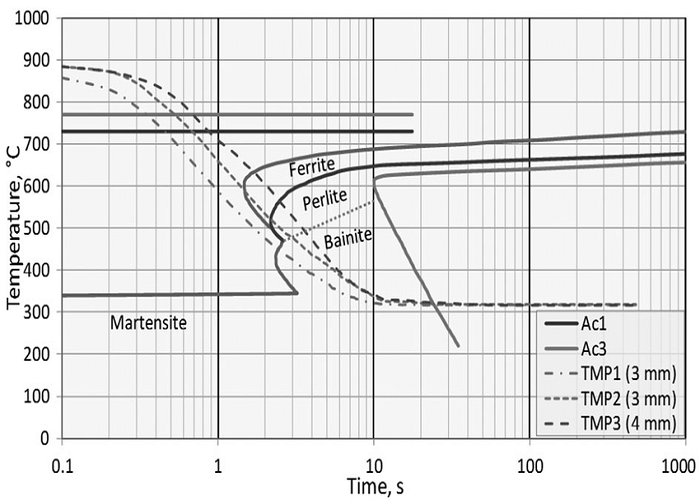
\includegraphics[width = 0.6\textwidth]{Figures/Cap2/CCT_SOA.png}
    \caption[Diagrama CCT de um aço CK45]%
    {Diagrama CCT de um ensaio de arrefecimento de um aço CK45, austenitizado à 880\textdegree C por 5 minutos\cite{Karli2016}.}
    \label{fig:CCT_SOA}
\end{figure}
%%%%%%%%%%%%%%%%%%%%%%%%%%%%%%%%%%%%%%%%%%%%%%%%%%%%%%%%%%%%%%%%%%%%%%%%%%%%%
\par
No entanto, nem sempre é possível realizar um ensaio para a realização de diagramas CCT, pelo que um grupo de pesquisadores tentou modelar por meio de algoritmos de \textit{machine learning}, baseado na composição química, as curvas de arrefecimento contínuo do material \cite{Martin2020}, portanto também é possível tentar prever a microestrutura final do material baseando-se na curva de arrefecimento e composição química. Para além disso, um outro parâmetro extremamente importante na microestrutura final de um material tratado termicamente, é a presença e quantidade de austenite residual, que da-se quando por exemplo, o material é arrefecido a uma taxa de resfriamento inadequada. Se o arrefecimento ocorrer muito rapidamente, a transformação completa da austenite pode ser dificultada.
%%%%%%%%%%%%%%%%%%%%%%%%%%%%%%%%%%%%%%%%%%%%%%%%%%%%%%%%%%%%%%%%%%%%%%%%%%%%%
\newpage
\subsection{Equações para previsão de temperaturas críticas}\label{ssec:previsao_martensite}
Outro fator que pode influenciar a presença de austenite residual é a temperatura de martensite final do material. Sendo esta muito baixa, não há possibilidade de toda a austenite ser transformada em martensite, portanto, resultando numa presença de austenite residual que pode não ser desejada na composição da microestrutura final. Existe, no entanto, uma maneira sugerida para prever as temperaturas de inicio de martensite(M\textsubscript{start}) e fim de martensite(M\textsubscript{finish}) pode ser vista nas Equações \ref{eq:Martensite_start} e \ref{eq:Martensite_finish}, respetivamente\cite{Honeycombe1995}.
%%%%%%%%%%%%%%%%%%%%%%%%%%%%%%%%%%%%%%%%%%%%%%%%%%%%%%%%%%%%%%%%%%%%%%%%%%%%%
\begin{equation}
    \label{eq:Martensite_start}
    \mathrm{M\textsubscript{(start)}}^{\circ}\mathrm{C} = 539-(423\%\mathrm{C})-(30,4\%\mathrm{Mn})-(17.7\%\mathrm{Ni})-(12,1\%\mathrm{Cr})-(7,7\%\mathrm{Mo})
\end{equation}
%%%%%%%%%%%%%%%%%%%%%%%%%%%%%%%%%%%%%%%%%%%%%%%%%%%%%%%%%%%%%%%%%%%%%%%%%%%%%
%%%%%%%%%%%%%%%%%%%%%%%%%%%%%%%%%%%%%%%%%%%%%%%%%%%%%%%%%%%%%%%%%%%%%%%%%%%%%
\begin{equation}
    \label{eq:Martensite_finish}
    \mathrm{M\textsubscript{(finish)}}^{\circ}\mathrm{C} = 346 - (474\%\mathrm{C}) - (33\%\mathrm{Mn}) - (17\%\mathrm{Ni}) - (21\%\mathrm{Mo})
\end{equation}
%%%%%%%%%%%%%%%%%%%%%%%%%%%%%%%%%%%%%%%%%%%%%%%%%%%%%%%%%%%%%%%%%%%%%%%%%%%%%
\par
Também é possível estimar as temperaturas de austenitização inicial(A\textsubscript{C1}) e final (A\textsubscript{C3}) através das equações \ref{eq:A_C1} e \ref{eq:A_C3}, respetivamente\cite{Platl2020}. No entanto, da mesma maneira que as equações para as temperaturas de martensite, estas são apenas estimativas e sempre que possível, deve-se optar pela realização de um ensaio experimental para determinar as temperaturas de transformação da microestrutura.
%%%%%%%%%%%%%%%%%%%%%%%%%%%%%%%%%%%%%%%%%%%%%%%%%%%%%%%%%%%%%%%%%%%%%%%%%%%%%
\begin{equation}
    \label{eq:A_C1}
    \mathrm{A\textsubscript{(C1)}}^{\circ}\mathrm{C} = 723 - (10,7\%\mathrm{Mn}) - (19,9\%\mathrm{Ni}) + (29.1\%\mathrm{Si}) + (6,38\%\mathrm{W})
\end{equation}
%%%%%%%%%%%%%%%%%%%%%%%%%%%%%%%%%%%%%%%%%%%%%%%%%%%%%%%%%%%%%%%%%%%%%%%%%%%%%
%%%%%%%%%%%%%%%%%%%%%%%%%%%%%%%%%%%%%%%%%%%%%%%%%%%%%%%%%%%%%%%%%%%%%%%%%%%%%
\begin{equation}
    \label{eq:A_C3}
    \begin{aligned}
    \mathrm{A\textsubscript{(C3)}}^{\circ}\mathrm{C} = {}   & 910 - (230\sqrt{\%\mathrm{C}}) - (15,2\%\mathrm{Ni}) + (44.7\%\mathrm{Si})\\
                                                            & + (104\%\mathrm{V}) + (31,5\%\mathrm{Mo}) + (6,38\%\mathrm{W})
\end{aligned}
\end{equation}
%%%%%%%%%%%%%%%%%%%%%%%%%%%%%%%%%%%%%%%%%%%%%%%%%%%%%%%%%%%%%%%%%%%%%%%%%%%%%
\par
Essas equações de previsão das temperaturas críticas são desenvolvidas com base em estudos experimentais e modelos termodinâmicos, levando em consideração as composições químicas e as características do material. Com os valores das temperaturas críticas, e com as curvas de transformação de fase mencionadas acima, é possível desenvolver um diagrama CCT estimado, sem a necessidade da realização de ensaios.
%%%%%%%%%%%%%%%%%%%%%%%%%%%%%%%%%%%%%%%%%%%%%%%%%%%%%%%%%%%%%%%%%%%%%%%%%%%%%
\subsection{Equações para previsão de dureza}\label{ssec:previsao_dureza}
Outro uso interessante das velocidades de arrefecimento, para além da previsão da microestrutura final, é a estimativa teórica da dureza final de um aço após um tratamento térmico. Uma estudo apresenta um modelo matemático gerado por um algoritmo computacional para tentar prever a dureza de um aço de acordo com a sua composição química, a velocidade de arrefecimento a que foi submetido, e a microestrutura final\cite{Trzaska2016}. As Equações \ref{eq:HV_fe} e \ref{eq:HV_ma}, indicam a estimativa de dureza consoante a velocidade de arrefecimento e elementos de liga para estruturas ferríticas e martensíticas, respetivamente.
%%%%%%%%%%%%%%%%%%%%%%%%%%%%%%%%%%%%%%%%%%%%%%%%%%%%%%%%%%%%%%%%%%%%%%%%%%%%%
\begin{equation}
    \begin{aligned}
    \mathrm{HV\textsubscript{(ferrite)}} = {}   & -73 + (253\%\mathrm{C}) + (52\%\mathrm{Mn}) + (10\%\mathrm{Si}) + (36\%\mathrm{Cr}) + (8\%\mathrm{Ni})\\
                                                & + (20\%\mathrm{Mo}) + (80\%\mathrm{V}) + (0,11\%\mathrm{A\textsubscript{C1}}) + (12,5\%\mathrm{Vc\textsuperscript{1/4}})
    \end{aligned}
    \label{eq:HV_fe}
\end{equation}
%%%%%%%%%%%%%%%%%%%%%%%%%%%%%%%%%%%%%%%%%%%%%%%%%%%%%%%%%%%%%%%%%%%%%%%%%%%%%
%%%%%%%%%%%%%%%%%%%%%%%%%%%%%%%%%%%%%%%%%%%%%%%%%%%%%%%%%%%%%%%%%%%%%%%%%%%%%
\begin{equation}
    \begin{aligned}
    \mathrm{HV\textsubscript{(martensite)}} = {}    & 200 + (824\sqrt{\%\mathrm{C}}) + (44\%\mathrm{Mn}) + (14\%\mathrm{Cr}) + (9\%\mathrm{Ni})\\
                                                    &+ (171\%\mathrm{V}) + (0,11\%\mathrm{Cu}) + (4,13\%\mathrm{Vc\textsuperscript{1/4}})
    \end{aligned}
    \label{eq:HV_ma}
\end{equation}
%%%%%%%%%%%%%%%%%%%%%%%%%%%%%%%%%%%%%%%%%%%%%%%%%%%%%%%%%%%%%%%%%%%%%%%%%%%%%
\par
Este modelo, claro, tem suas limitações, pelo que está desenvolvido para um intervalo de percentagens de elementos de liga, e tem melhores resultados quando os valores estão mais próximos da média, no entanto, com erros absolutos por volta dos 20-30HVs, esta pode ser uma ferramenta valiosa para a previsão das durezas de um material quando se está a alterar os parâmetros de tratamento. 

%%%%%%%%%%%%%%%%%%%%%%%%%%%%%%%%%%%%%%%%%%%%%%%%%%%%%%%%%%%%%%%%%%%%%%%%%%%%%
\newpage
\subsection{Espectrometria de descarga luminescente ótica por emissão de gás}\label{ssec:soa_espectrometria}
A espectrometria de descarga luminescente ótica por emissão de gás (GDOES) é uma técnica analítica poderosa para análise de elementos e perfis de profundidade em materiais sólidos.
\par
A GDOES baseia-se na criação de um plasma, um estado altamente energético da matéria, a partir de uma descarga de gás numa pequena área do material a ser analisado. O gás, geralmente árgon, é ionizado por uma descarga elétrica (Ver Figura \ref{fig_GDOES_A_C}), formando um plasma que interage com a superfície do material. As partículas de árgon colidem com a superfície do material, causando a erosão da superfície e a formação de um plasma secundário a partir do material. É importante notar que a GDOES é uma técnica destrutiva, uma vez que envolve a erosão da superfície do material.
%%%%%%%%%%%%%%%%%%%%%%%%%%%%%%%%%%%%%%%%%%%%%%%%%%%%%%%%%%%%%%%%%%%%%%%%%%%%%
\begin{figure}[htb]
    \centering
    \begin{subfigure}{.4\textwidth}
      \centering
      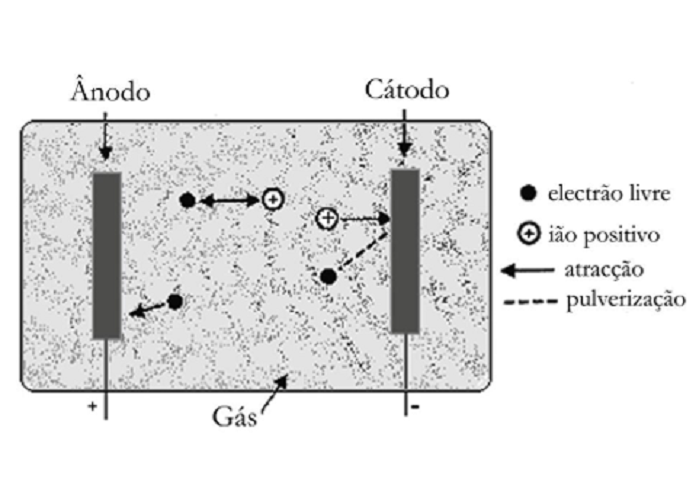
\includegraphics[width = 0.9\linewidth]{Figures/Cap2/GDOES_A_C.png}
      \caption{}
      \label{fig_GDOES_A_C}
    \end{subfigure}%
    \begin{subfigure}{.4\textwidth}
      \centering
      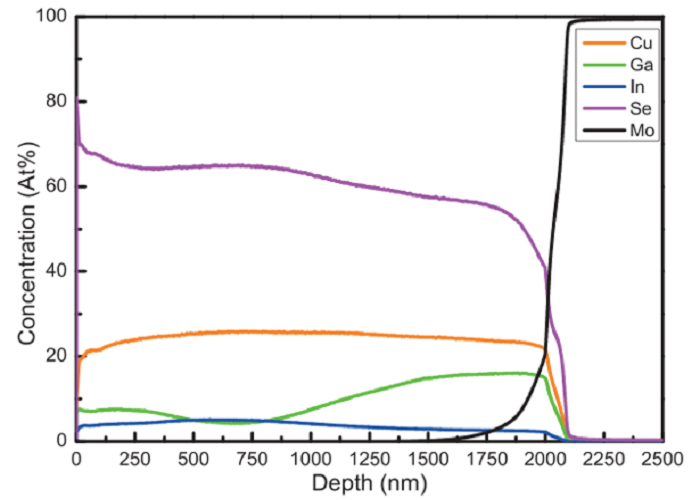
\includegraphics[width = 0.9\linewidth]{Figures/Cap2/GDOES_comp.png}
      \caption{}
      \label{fig:GDOES_comp}
    \end{subfigure}
    \caption[Funcionamento e resultados de um GDOES]%
    {À esquerda, Esquema de formação de um plasma GDOES, retirado de \cite{Santos2009}. À direita, Gráfico com resultado de uma espectroscopia, retirado de \cite{Covalent2022}.}
\end{figure}
%%%%%%%%%%%%%%%%%%%%%%%%%%%%%%%%%%%%%%%%%%%%%%%%%%%%%%%%%%%%%%%%%%%%%%%%%%%%%
\par
A luz emitida por este plasma secundário é coletada e o espectro formado é analisado. Cada elemento na amostra emite luz a um conjunto específico de comprimentos de onda, permitindo assim a determinação da composição elementar da amostra. A intensidade da emissão em cada comprimento de onda é proporcional à quantidade do elemento na amostra, permitindo uma análise quantitativa dos elementos presentes \cite{Saraiva2015}. Além disso, a composição elementar pode ser monitorizada ao longo do tempo, fornecendo um perfil de profundidade da composição do material, como pode ser visto na Figura \ref{fig:GDOES_comp}.
\par
Portanto, quando não se tem a certeza da composição química de uma liga metálica, por exemplo, após um tratamento de carbonitruração, pode-se realizar um ensaio de GDOES de forma a perceber a quantidade de carbono e azoto, e também outros elementos de liga, estão presentes no material, e as suas proporções em relação à profundidade.
    \chapter{Materiais e Métodos} \label{ch:materiais}
\setlength{\headheight}{13.6pt}
%%%%%%%%%%%%%%%%%%%%%%%%%%%%%%%%%%%%%%%%%%%%%%%%%%%%%%%%%%%%%%%%%%%%%%%%%%%%%
\section{Introdução} \label{sec:materiais_intro}
Como já foi referido, o principal objetivo deste trabalho é desenvolver uma ferramenta porta-peças para proteger o diâmetro interno das rodas de coroa \textbf{BD35}, \textbf{DB45} e \textbf{JT4}, de forma a melhorar a operação de torneamento duro e diminuir a ocorrência de não conformidades devidas à fissurações a frio. 
\par
Assim, este capítulo começa por descrever o \textbf{caso de estudo}, isto é, as rodas de coroa em que será feito o processo de carbonitruração e seu processo de maquinação antes deste processo(que é mencionado a seguir como “processo de obtenção da peça branca”), as ferramentas porta-peças atualmente utilizadas no processo de carbonitruração das rodas de coroa supracitadas(que a partir deste ponto são chamadas peças negras), e o processo de torneamento, onde é obtida a geometria final das rodas de coroa que posteriormente serão prensadas e soldadas à caixa diferencial.
\par
É então apresentado o processo de simulação por CFD que as rodas de coroa serão sujeitos, para a linha de série e para todas as soluções propostas, e em seguida, é apresentada uma solução inicial, chamada de \textbf{“Tampa P”}, simples, onde as únicas diferenças desta solução para a ferramenta atualmente utilizada são a modificação da \textit{falsa coroa} para não permitir a passagem de fluido \textbf{por baixo} e a adição de uma \textit{tampa} \textbf{em cima} com efeito análogo. Somado a isto, são apresentadas três soluções complementares, cujo objetivo é melhorar alguns parâmetros obtidos no ensaio da solução inicial \textbf{“P”}, no caso das tampas \textbf{“Y”} e \textbf{“O”}, ou simplificar o sistema, no caso da solução \textbf{“Sem tampa”}.
\par
Por fim, são descritos os \textbf{parâmetros de conformidade} e o processo de ensaio para verificação dos impactos das várias modificações, que posteriormente serão analisados e discutidos no capítulo \ref{ch:resultados}, e uma vez que estes serão utilizados para validar os parâmetros de conformidade, serão também apresentados os métodos de ensaio de dureza, de verificação dimensional e o ensaio de difusibilidade do hidrogénio.
\newpage
%%%%%%%%%%%%%%%%%%%%%%%%%%%%%%%%%%%%%%%%%%%%%%%%%%%%%%%%%%%%%%%%%%%%%%%%%%%%%
\section{Caso de estudo} \label{sec:materiais_CS}
\subsection{Processo de obtenção da peça branca} \label{ssec:materiais_CS_peca_branca}

O processo de produção da peça branca, inicia-se com um bruto de aço de baixa liga \textbf{AFNOR 27MC5}, ou \textbf{EN-1.7149}. Cada série de rodas de coroa tem um bruto de dimensões específicas, bem como programas de maquinação e padrões de conformidade específicos. Como exemplo, na Figura \ref{fig:Bruto_desenho} vê-se as dimensões do bruto das rodas de coroa DB45 de aproximadamente 204,4 mm de diâmetro externo, 106 mm de diâmetro interno e 39 mm de espessura.

%%%%%%%%%%%%%%%%%%%%%%%%%%%%%%%%%%%%%%%%%%%%%%%%%%%%%%%%%%%%%%%%%%%%%%%%%%%%%
\begin{figure}[htb]
    \centering
    \begin{subfigure}{.5\textwidth}
        \centering
        \includegraphics[width = 0.9\textwidth]{Figures/Cap3/Bruto_fotografia.png}
        \caption{}
        \label{fig:Bruto_fotografia}
    \end{subfigure}%
    \begin{subfigure}{.5\textwidth}
        \centering
        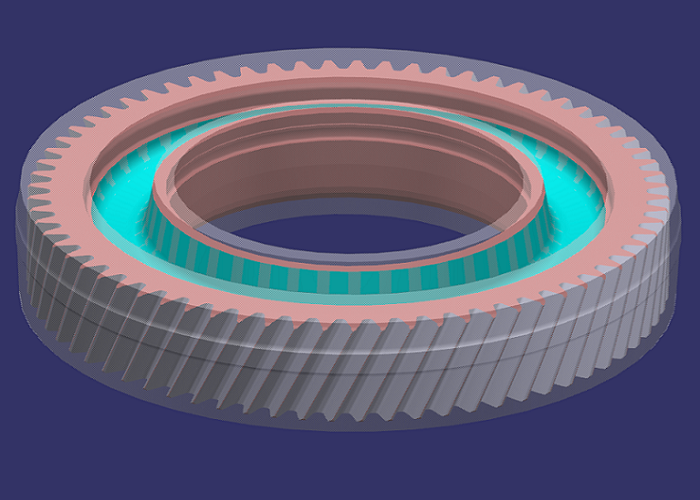
\includegraphics[width = 0.9\textwidth]{Figures/Cap3/Bruto_CAD.png}
        \caption{}
        \label{fig:Bruto_desenho}
    \end{subfigure}
    \caption[Imagens do bruto para fabricação da peça branca]%
    {À esquerda, uma fotografia de um bruto utilizado para obter a peça branca. À direita, um desenho com as dimensões do bruto e hachuras com o formato e dimensões da peça branca final.}
\end{figure}
%%%%%%%%%%%%%%%%%%%%%%%%%%%%%%%%%%%%%%%%%%%%%%%%%%%%%%%%%%%%%%%%%%%%%%%%%%%%%

\par
Deste bruto, serão removidos os excessos de material do diâmetro interno, das faces superior e inferior, e maquinado o dentado, tudo isto feito de forma automática, sendo apenas necessária a intervenção do operador na alimentação inicial dos brutos na linha de produção, na troca das ferramentas, seja por desgaste ou por mudança da série a maquinar, ou em casos de defeitos de máquina. Cada operação é realizada num centro de maquinagem diferente, e o transporte é realizado por meio de transportadores mecânicos, o que torna o processo mais ágil e permite a continuação do processo produtivo em caso de avaria de algum dos centros.

\par
Após estarem maquinadas as rodas de coroa, estas estão prontas para seguir para o processo de carbonitruração, processo que tornar-lhes-á peças negras. Portanto, após a saída do último centro de maquinagem, as rodas de coroa são direcionadas a uma ilha em que um braço mecânico carrega de forma ordenada uma carga, composta por três pratos de cinco colunas cada, totalizando quinze colunas por carga. O número de rodas de coroa por coluna varia entre 10, no caso das séries “DB45” e 11, no caso das séries “DB35” e “JT4”. Isto é devido ao peso máximo suportado pelo elevador do forno de carbonitruração, que tem um limite de 550kg. Sendo as séries “DB45” mais espessas, portanto, mais pesadas, existe a necessidade da redução do número de rodas de coroa de 55 para 50 por prato.
%%%%%%%%%%%%%%%%%%%%%%%%%%%%%%%%%%%%%%%%%%%%%%%%%%%%%%%%%%%%%%%%%%%%%%%%%%%%%
\begin{figure}[htb]
    \centering
    \begin{subfigure}{.45\textwidth}
        \centering
        \includegraphics[width = 0.9\textwidth]{Figures/Cap3/Peca_branca_fotografia.png}
        \caption[]%
        {}
        \label{fig:Peca_branca_fotografia}
    \end{subfigure}%
    \begin{subfigure}{.45\textwidth}
        \centering
        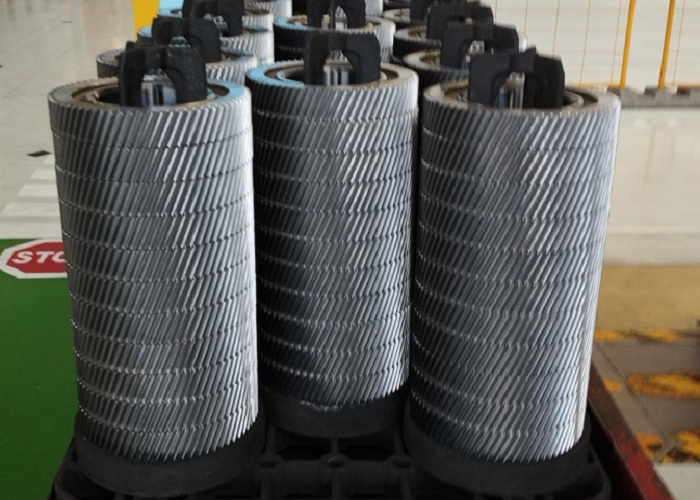
\includegraphics[width = 0.9\textwidth]{Figures/Cap3/Carga_fotografia.png}
        \caption{}
        \label{fig:Carga_peca_branca}
    \end{subfigure}
    \caption[Peça branca final e Prato de Rodas de coroa série DB35]%
    {À esquerda, uma fotografia de uma roda de coroa DB45 peça branca. À direita, uma fotografia de um prato montado com 50 rodas de coroa DB45 “peça branca” maquinadas.}
\end{figure}
%%%%%%%%%%%%%%%%%%%%%%%%%%%%%%%%%%%%%%%%%%%%%%%%%%%%%%%%%%%%%%%%%%%%%%%%%%%%%
\subsection{Processo de tratamentos térmicos} \label{ssec:materiais_CS_carbonitruracao}
Chegando a carga na zona dos tratamentos térmicos, esta é carregada para uma máquina de pré-oxidação, este processo precede a carbonitruração e é utilizado para melhorar a aderência da camada de carbono e azoto adquirida. Para uma melhor perceção do sistema, as Figuras \ref{fig:Prato}, \ref{fig:Torre} e \ref{fig:Falsa_coroa} ilustram as tres partes da ferramenta porta-peças atualmente utilizados em toda a linha dos tratamentos térmicos. O material dos componentes da ferramenta porta-peças é o \textbf{aço refratário EN 1.4807}.

%%%%%%%%%%%%%%%%%%%%%%%%%%%%%%%%%%%%%%%%%%%%%%%%%%%%%%%%%%%%%%%%%%%%%%%%%%%%%
\begin{figure}[htb]
    \centering
    \begin{subfigure}{.33\textwidth}\
        \centering
        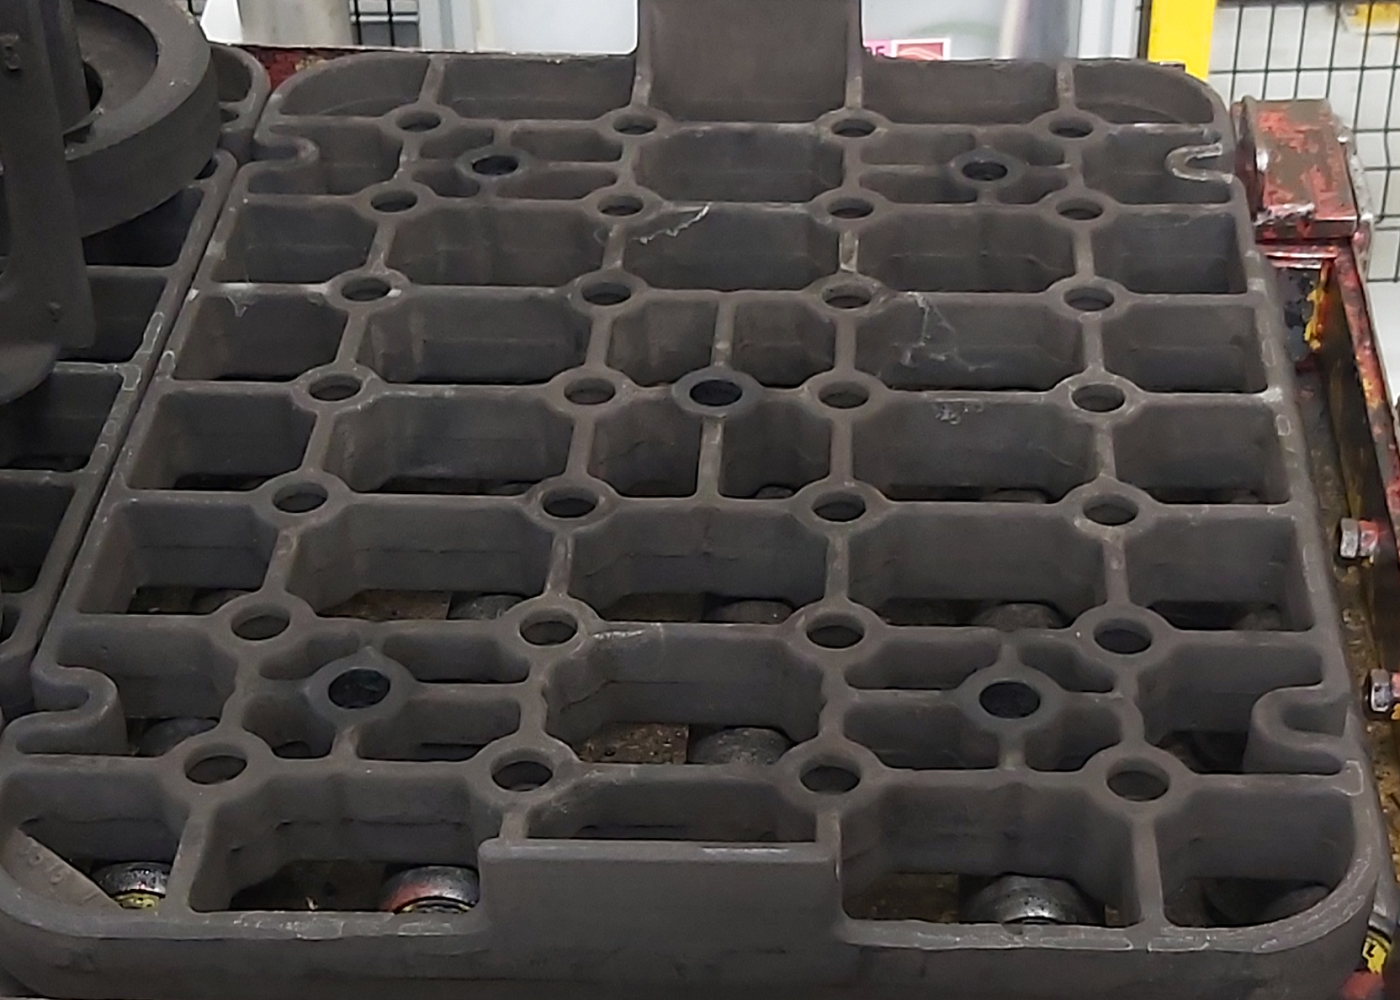
\includegraphics[width = 0.9\textwidth]{Figures/Cap3/Prato.png}
        \caption{}
        \label{fig:Prato}
    \end{subfigure}%
    \centering
    \begin{subfigure}{.33\textwidth}
        \centering
        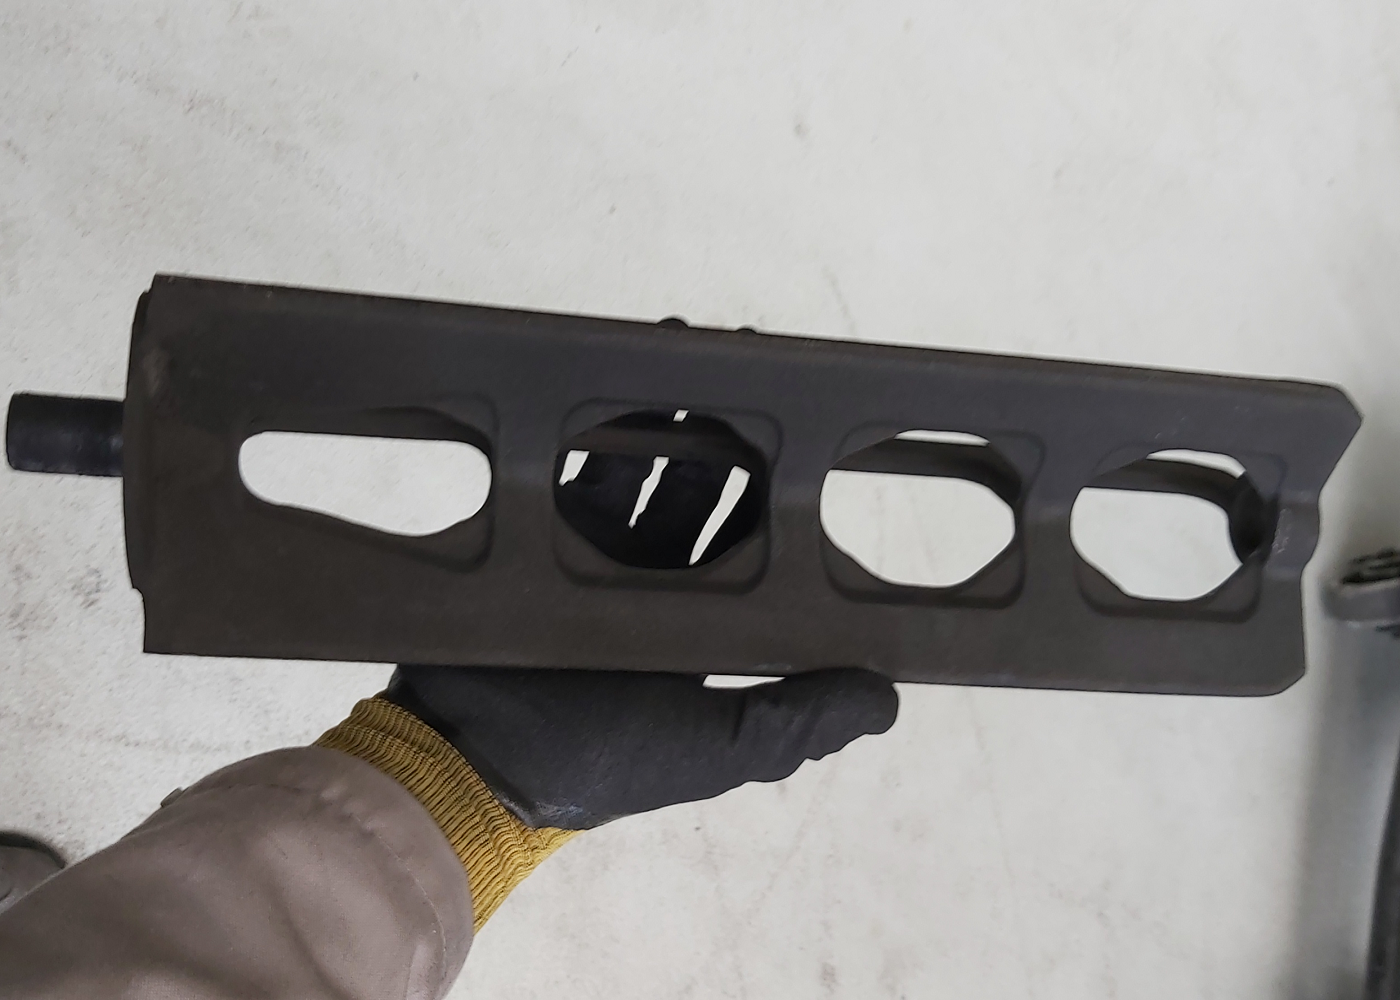
\includegraphics[width = 0.9\textwidth]{Figures/Cap3/Torre.png}
        \caption{}
        \label{fig:Torre}
    \end{subfigure}
    \centering
    \begin{subfigure}{.33\textwidth}
        \centering
        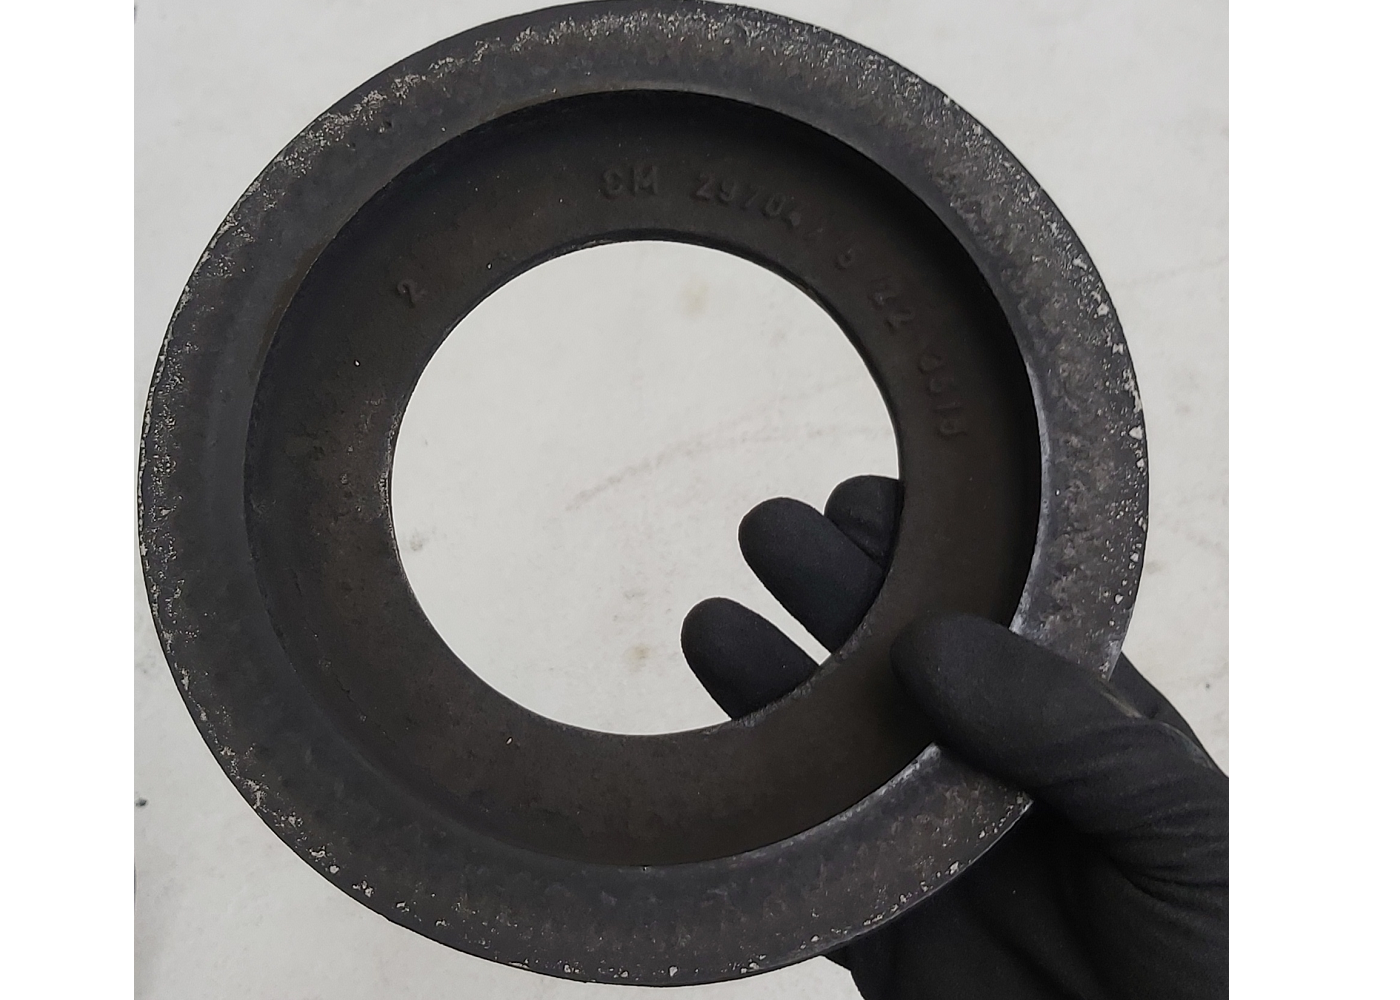
\includegraphics[width = 0.9\textwidth]{Figures/Cap3/Falsa_coroa.png}
        \caption{}
        \label{fig:Falsa_coroa}
    \end{subfigure}
    \caption[Fotografias dos tres componentes da ferramenta porta-peças]%
    {Fotografias do prato, da torre, e da falsa coroa da ferramenta porta-peças.}
\end{figure}
%%%%%%%%%%%%%%%%%%%%%%%%%%%%%%%%%%%%%%%%%%%%%%%%%%%%%%%%%%%%%%%%%%%%%%%%%%%%%
\par
A pré-oxidação é realizada ao aquecer o material a uma temperatura de 500\textdegree C por cerca de 90 minutos, num ambiente controlado, de forma a obter uma fina camada de óxidos na superfície das rodas de coroa que atua permitindo uma difusão mais controlada do carbono e do azoto na superfície do material durante a etapa de carbonitruração que resulta em uma distribuição mais uniforme destes elementos na camada formada, uniformizando as propriedades mecânicas adquiridas pelo processo. Para além disso, a camada de óxidos diminui a probabilidade de fissurações a quente, uma vez que funciona como um degrau de aquecimento e evita o choque térmico, já que o forno de carbonitruração encontra-se a temperaturas de quase 900\textdegree C. Por fim, a camada de óxidos também promove uma aderência mais forte entre a camada de carbonitruração e o núcleo metálico, o que diminui a probabilidade de ocorrência de descamações. Após esta etapa, as peças têm uma coloração característica, próxima do azul escuro, característica do processo de oxidação e da temperatura atingida neste processo.
\par
Logo após a pré-oxidação, as peças são conduzidas por transportadores mecânicos para um sitio de carregamento, para serem transportadas para o forno de carbonitruração. Neste forno, as peças são novamente aquecidas, desta vez a uma temperatura de 870\textdegree C, por um tempo de cerca de aproximadamente 180 minutos. Nesta etapa, as peças estão submetidas a uma atmosfera de aproximadamente 0,7\% Carbono e 20\% de Azoto, controladas por meio de um débito de amoníaco (NH\textsubscript{3}), metanol (CH\textsubscript{3}OH), propano (C\textsubscript{3}H\textsubscript{8}) e gás de azoto (N\textsubscript{2}). O processo é realizado numa câmara a uma pressão de 3 bar, de forma a permitir que a maior quantidade de átomos de carbono e azoto penetrem nas rodas de coroa.
%%%%%%%%%%%%%%%%%%%%%%%%%%%%%%%%%%%%%%%%%%%%%%%%%%%%%%%%%%%%%%%%%%%%%%%%%%%%%
\par
Após os aproximadamente 180 minutos no forno de carbonitruração, as peças são descarregadas do forno e rapidamente submergidas num tanque de têmpera de dimensões de base 700x700mm e  970mm de altura, num fluido de têmpera “Shell Voluta H300”, que encontra-se a aproximadamente 170\textdegree C durante cerca de 15 minutos. Após o processo de têmpera, as peças seguem para duas operações seguidas de lavagem, cada uma com duração de cerca de 90 minutos, e só então são submetidas à um processo de revenido, de forma a aliviar as tensões internas do material e adequar os valores de dureza e tenacidade às conformidade exigidas no produto final.
%%%%%%%%%%%%%%%%%%%%%%%%%%%%%%%%%%%%%%%%%%%%%%%%%%%%%%%%%%%%%%%%%%%%%%%%%%%%%
\begin{figure}[htb]
    \centering
    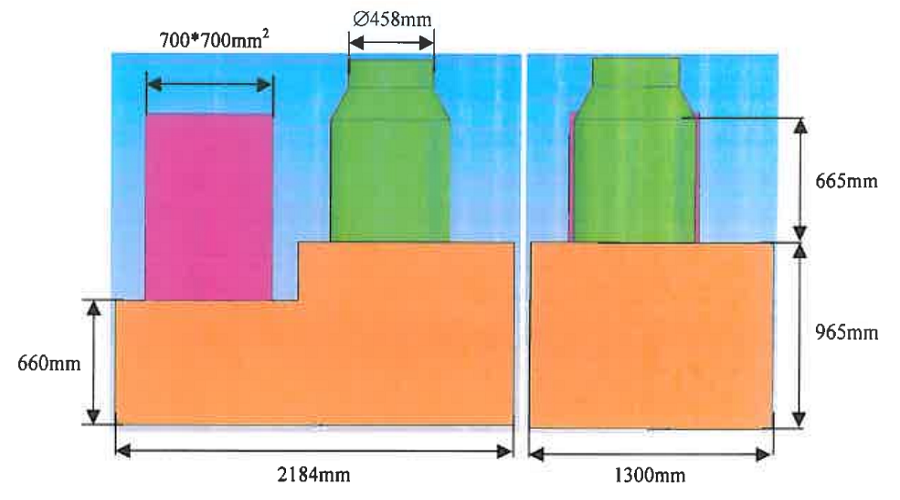
\includegraphics[width = 0.6\textwidth]{Figures/Cap3/Tanque_Tempera.png}
    \caption[Tanque de têmpera]%
    {Imagem esquemática do tanque de têmpera no qual é realizada a têmpera das rodas de coroa.}
    \label{fig:tanque_tempera}
\end{figure}
%%%%%%%%%%%%%%%%%%%%%%%%%%%%%%%%%%%%%%%%%%%%%%%%%%%%%%%%%%%%%%%%%%%%%%%%%%%%%

\par
O revenido é realizado durante 5 horas, em 5 zonas seguidas de 60 minutos cada, a 190\textdegree C, sendo então arrefecido lentamente à saída do forno de revenido. Após o arrefecimento das rodas de coroa, estas então são inseridas num processo de granalhagem, de forma limpar os contaminantes que restem dos processos anteriores, como resquícios de óleo não removidos no processo de lavagem, sobras de detergente ou camadas superficiais de óxidos. Uma vez que o processo de granalhagem é concluído, as rodas de coroa são conduzidas à linha de torneamento duro, onde serão removidas imperfeições e deformações resultantes do processo de obtenção da peça negra.

%%%%%%%%%%%%%%%%%%%%%%%%%%%%%%%%%%%%%%%%%%%%%%%%%%%%%%%%%%%%%%%%%%%%%%%%%%%%%
\newpage
\subsection{Processo de torneamento duro} \label{ssec:materiais_CS_torneamento}
Uma vez que as peças negras tem uma dureza superficial extremamente alta, por volta dos 700HV, é necessária a utilização de ferramentas e parâmetros de corte especiais para obter os requisitos dimensionais nas rodas de coroa. Para este efeito, são utilizadas pastilhas com revestimento de nitreto de boro cúbico (CBN), material este que pode atingir até 2000\textdegree C sem grandes perdas de dureza e em temperatura ambiente, apresenta valores de dureza por volta dos 1100HV. Neste processo, o diâmetro interno das rodas de coroa é torneada a zona de soldadura, a zona de prensagem, e é feito um rasgo para a zona de escapamento de gases de soldadura. As dimensões das rodas de coroa antes e depois do torneamento duro podem ser vistas nas Figuras \ref{fig:Coroa_antes_torneamento} e \ref{fig:Coroa_apos_torneamento}.
%%%%%%%%%%%%%%%%%%%%%%%%%%%%%%%%%%%%%%%%%%%%%%%%%%%%%%%%%%%%%%%%%%%%%%%%%%%%%
\begin{figure}[htb]
    \centering
    \begin{subfigure}{.5\textwidth}\
        \centering
        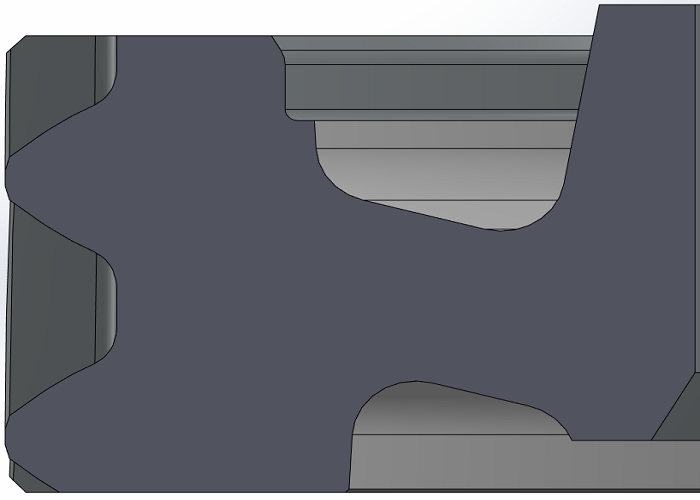
\includegraphics[width = 0.9\textwidth]{Figures/Cap3/DB45_antes_torn.png}
        \caption{}
        \label{fig:Coroa_antes_torneamento}
    \end{subfigure}%
    \begin{subfigure}{.5\textwidth}
        \centering
        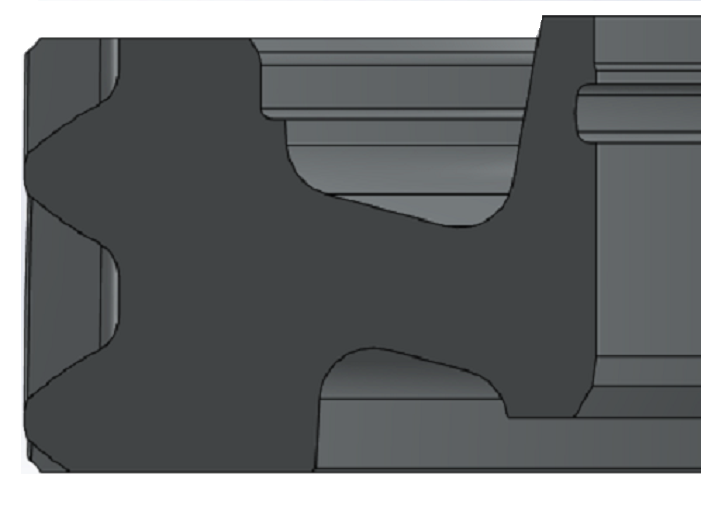
\includegraphics[width = 0.9\textwidth]{Figures/Cap3/DB45_apos_torn.png}
        \caption{}
        \label{fig:Coroa_apos_torneamento}
    \end{subfigure}
    \caption[Imagens das rodas de coroa antes e após o torneamento duro]%
    {À esquerda, um esquema das dimensões das rodas de coroa DB45 antes do torneamento duro. À direita, o mesmo esquema após a operação de torneamento duro, em vermelho, a zona de torneamento.}
\end{figure}
%%%%%%%%%%%%%%%%%%%%%%%%%%%%%%%%%%%%%%%%%%%%%%%%%%%%%%%%%%%%%%%%%%%%%%%%%%%%%

\par
Um dos problemas abordados neste projeto é justamente o custo da operação de torneamento duro. Os custos da ferramenta e a baixa quantidade de operações realizadas por cada ferramenta que resultam num tempo considerável em que a máquina não está a trabalhar e o alto consumo energético devido às condições de corte, que são maioritariamente causados pela alta dureza no diâmetro interno das rodas de coroa. 
%%%%%%%%%%%%%%%%%%%%%%%%%%%%%%%%%%%%%%%%%%%%%%%%%%%%%%%%%%%%%%%%%%%%%%%%%%%%%
\par
Sendo assim, havendo a possibilidade da redução desta dureza, existe uma margem para a diminuição dos custos de operação, seja com a mudança da ferramenta para uma alternativa de menor custo, pelo aumento da quantidade de operações realizadas por cada ferramenta, pela alteração dos parâmetros de corte de forma a reduzir o consumo energético ou o tempo de ciclo, ou até por uma junção de todas as possibilidades anteriores.
%%%%%%%%%%%%%%%%%%%%%%%%%%%%%%%%%%%%%%%%%%%%%%%%%%%%%%%%%%%%%%%%%%%%%%%%%%%%%
\subsection{Prensagem e Soldadura} \label{ssec:materials_CS_prens_e_sold}
Após o torneamento duro, as rodas de coroa são prensadas para em sequencia serem soldadas às caixas diferenciais, estas “caixas nuas”, em ferro fundido EN-GJS-600-10 são também produzidas na fábrica, no entanto, não sendo estas escopo deste projeto, seu processo produtivo não será abordado neste documento. Cada série de roda de coroa tem uma série de caixa diferencial designada, como exemplo, vê-se uma caixa diferencial “nua” na Figura \ref{fig:Caixa_nua_DB45}, e uma caixa diferencial montada na Figura \ref{fig:Caixa_montada_DB45}.
\newpage
%%%%%%%%%%%%%%%%%%%%%%%%%%%%%%%%%%%%%%%%%%%%%%%%%%%%%%%%%%%%%%%%%%%%%%%%%%%%%
\begin{figure}[htb]
    \centering
    \begin{subfigure}{.5\textwidth}\
        \centering
        \includegraphics[width = 0.9\textwidth]{Figures/Cap3/Caixa_nua.png}
        \caption[]%
        {}
        \label{fig:Caixa_nua_DB45}
    \end{subfigure}%
    \begin{subfigure}{.5\textwidth}
        \centering
        \includegraphics[width = 0.9\textwidth]{Figures/Cap3/Caixa_montada.png}
        \caption{}
        \label{fig:Caixa_montada_DB45}
    \end{subfigure}
    \caption[Caixa diferencial “nua”, e caixa diferencial montada.]%
    {À esquerda, uma fotografia de uma caixa diferencial “nua” antes de ser prensada a uma roda de coroa. À direita, uma caixa diferencial já prensada.}
\end{figure}
%%%%%%%%%%%%%%%%%%%%%%%%%%%%%%%%%%%%%%%%%%%%%%%%%%%%%%%%%%%%%%%%%%%%%%%%%%%%%
\par
Portanto, sendo prensadas a roda de coroa e caixa diferencial “nua”, a caixa diferencial deverá ser soldada, neste caso uma soldadura à laser com adição de INCONEL-82. Como referido no Subcapítulo \ref{ssec:soldadura-soldabilidade}, pode-se utilizar a correlação de Graville da Figura \ref{fig:Graville} para tentar prever a probabilidade de ocorrência de fissuração por hidrogénio no conjunto. Novamente, é importante referir que fissurações a hidrogénio são causadas por 3 fatores; microestrutura suscetível, neste caso, uma grande quantidade de martensite; uma fonte de hidrogénio difusível, neste caso, a atmosfera rica em hidrogénio da carbonitruração; e tensões residuais do processo de soldadura. Na Figura \ref{fig:microestrutura_diametro_serie} é possível verificar que o diâmetro interno das rodas de coroa estão preenchidas por microestruturas de martensite e austenite residual, com maior quantidade de austenite residual na extremidade mais próxima da superfície de tratamento. Isto pode ser explicado pela temperatura final de martensite de um aço ser mais baixa quanto maior a composição de carbono, e sendo a presença de carbono tão maior quanto menor for a profundidade observada, há uma maior presença de carbono na superfície, portanto, uma maior quantidade de austenite que não foi transformada.
%%%%%%%%%%%%%%%%%%%%%%%%%%%%%%%%%%%%%%%%%%%%%%%%%%%%%%%%%%%%%%%%%%%%%%%%%%%%%
\begin{figure}[htb]
    \centering
    \begin{subfigure}{.5\textwidth}\
        \centering
        
\includegraphics[width = 0.9\textwidth]{Figures/Cap3/Falta_Imagem.png}
        \caption{}
        \label{fig:microestrutura_diametro_serie}
    \end{subfigure}%
    \begin{subfigure}{.5\textwidth}
        \centering
        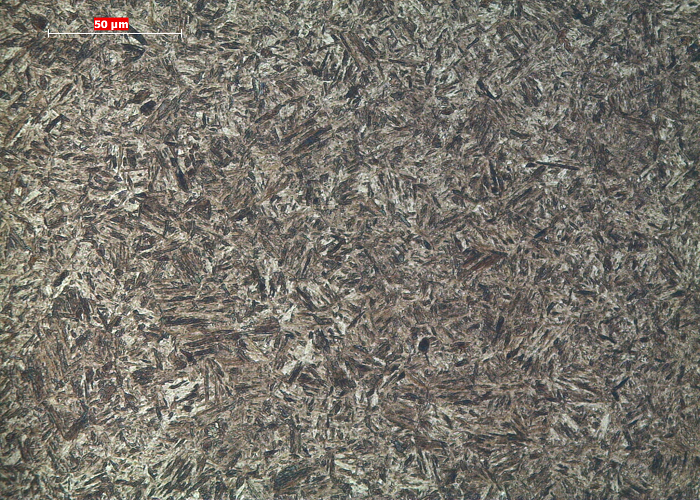
\includegraphics[width = 0.9\textwidth]{Figures/Cap3/Microestrutura_serie.png}
        \caption{}
        \label{fig:imagem_diametro_serie}
    \end{subfigure}
    \caption[Microestrutura e perfil do diâmetro interno.]%
    {À esquerda, uma imagem da microestrutura da peça branca. À direita, uma imagem da microestrutura de uma roda de coroa DB45 após têmpera.}
\end{figure}
%%%%%%%%%%%%%%%%%%%%%%%%%%%%%%%%%%%%%%%%%%%%%%%%%%%%%%%%%%%%%%%%%%%%%%%%%%%%%
%%%%%%%%%%%%%%%%%%%%%%%%%%%%%%%%%%%%%%%%%%%%%%%%%%%%%%%%%%%%%%%%%%%%%%%%%%%%%
\newpage
\par
Uma vez que os parâmetros de \% C e CE dos materiais da roda de coroa e da caixa “nua”, são importantes para perceber a suscetibilidade de fissuração por hidrogénio, a Tabela \ref{tab:Comp_materiais} indica a composição indicativa do aço 27MC5, das rodas de coroa, e do ferro fundido EN-GJS-600-10 das caixas diferenciais “nuas”. É importante referir que para o calculo posterior do CE, nas Equações \ref{eq:CE_calculado_27MC5} e \ref{eq:CE_calculado_GJS-600-10}, são utilizados os valores médios de cada elemento da composição do material, o que pode causar alguma diferença em materiais cuja composição se encontre numa posição mais extrema do espectro de conformidades. No entanto, uma vez que este espectro não é demasiado vasto, pode-se utilizar a média como visualização da soldabilidade deste material. Para além disso, é também utilizado o percentual de carbono após a carbonitruração, de 0,7\% , uma vez que a zona afetada termicamente das rodas de coroa de série é enriquecida por carbonitruração.
%%%%%%%%%%%%%%%%%%%%%%%%%%%%%%%%%%%%%%%%%%%%%%%%%%%%%%%%%%%%%%%%%%%%%%%%%%%%%
\begin{table}[htb]
    \centering
    \caption[Composição dos materiais da caixa diferencial]%
    {Valores de conformidade da composição dos materiais constituintes das rodas de coroa e caixas “nuas”.}
    \label{tab:Comp_materiais}
    \begin{tabular}{lrr} 
    \toprule
    \textbf{Elemento de liga} & \multicolumn{1}{c}{\textbf{Composição 27MC5 (\%)}} & \multicolumn{1}{c}{\textbf{Composição GJS-600-10 (\%)}}  \\ 
    \hline\hline
    Carbono (C)      & 0,23 à 0,31                               & 3,1 à 3,4                                       \\
    Manganês (Mn)    & 1,10 à 1,40                               & Até 0,5                                         \\
    Níquel (Ni)      & Até 0,30                                  & Não especificado                                \\
    Vanádio (V)      & Não especificado                          & Não especificado                                \\
    Molibdénio (Mo)  & Não especificado                          & Não especificado                                \\
    Crómio (Cr)      & 1,00 à 1,40                               & Não especificado                                \\
    Cobre (Cu)       & Até 0,40                                  & Até 0,15                                        \\
    Titânio (Ti)     & Até 0,010                                 & Não especificado                                \\
    Alumínio (Al)    & Até 0,050                                 & Não especificado                                \\
    Silício (Si)     & Até 0,40                                  & 4,1 à 4,5                                       \\
    Enxofre (S)      & 0,020 à 0,040                             & Até 0,02                                        \\
    Fósforo (P)      & Até 0,025                                 & Até 0,05                                        \\
    Estanho (Sn)     & Não especificado                          & Até 0,05                                        \\
    \bottomrule
    \end{tabular}
    \end{table}
%%%%%%%%%%%%%%%%%%%%%%%%%%%%%%%%%%%%%%%%%%%%%%%%%%%%%%%%%%%%%%%%%%%%%%%%%%%%%
%%%%%%%%%%%%%%%%%%%%%%%%%%%%%%%%%%%%%%%%%%%%%%%%%%%%%%%%%%%%%%%%%%%%%%%%%%%%%
\begin{equation}
    \centering
    \label{eq:CE_calculado_27MC5}
    \mathrm{CE\textsubscript{(27MC5)}} = 0,7 + \frac{1,25}{6}+\frac{1,20+0+0}{5}+\frac{0,20+0,15}{15}
\end{equation}
%%%%%%%%%%%%%%%%%%%%%%%%%%%%%%%%%%%%%%%%%%%%%%%%%%%%%%%%%%%%%%%%%%%%%%%%%%%%%
%%%%%%%%%%%%%%%%%%%%%%%%%%%%%%%%%%%%%%%%%%%%%%%%%%%%%%%%%%%%%%%%%%%%%%%%%%%%%
\begin{equation}
    \centering
    \label{eq:CE_calculado_GJS-600-10}
    \mathrm{CE\textsubscript{(GJS-600-10)}} = 3,25 + \frac{0,25}{6}+\frac{0+0+0}{5}+\frac{0,08+0}{15}
\end{equation}
%%%%%%%%%%%%%%%%%%%%%%%%%%%%%%%%%%%%%%%%%%%%%%%%%%%%%%%%%%%%%%%%%%%%%%%%%%%%%
\par
Com isto, temos que os valores de \%C e CE são, respetivamente 0,7 e 1,17 para o aço, e 3,25 e 3,3 para o ferro fundido. Quando comparados com os valores de referencia descritos na Tabela \ref{tab:CE}, ambos os materiais tem uma má soldabilidade, somado a isto, a martensite tem uma má condutividade térmica quando comparada com outras microestruturas do aço. 
\par
Ainda que usemos o valor de referencia para o percentual de carbono do aço sem tratamento termoquímico, temos um valor de CE de 0,72, o que ainda seria considerado um material com má soldabilidade. Devido a estes problemas, os parâmetros de soldadura são minuciosamente selecionados de forma a permitir uma boa formação da ZAT e uma penetração total da zona de soldadura, sendo o principal parâmetro para a obtenção destes resultados numa soldadura a laser a potencia de soldadura.
\newpage
\par
Para além disso, se utilizarmos a correlação de Graville, da Figura \ref{fig:Graville}, ambos os materiais têm uma grande probabilidade de ocorrência de fissuração, e o facto de serem peças de revolução, torna estas peças especialmente suscetíveis à fissurações, devido a zona de recobrimento (Figura \ref{fig:recobrimento}). Uma vez que a zona de inicio e término de soldadura da-se no mesmo ponto, esta zona sofre o equivalente a uma soldadura de dois passes. 
%%%%%%%%%%%%%%%%%%%%%%%%%%%%%%%%%%%%%%%%%%%%%%%%%%%%%%%%%%%%%%%%%%%%%%%%%%%%%
\begin{figure}[htb]
    \centering
    \includegraphics[width = 0.52\textwidth]{Figures/Cap3/Recobrimento.png}
    \caption[Zona de recobrimento de uma roda de coroa DB45]%
    {Fotografia de uma roda de coroa DB45 após o processo de soldadura, com destaque em vermelho para a zona de recobrimento.}
    \label{fig:recobrimento}
\end{figure}
%%%%%%%%%%%%%%%%%%%%%%%%%%%%%%%%%%%%%%%%%%%%%%%%%%%%%%%%%%%%%%%%%%%%%%%%%%%%%
\par
A adição de carbono, azoto, e a eventual adição de hidrogénio no forno de carbonitruração, e a transformação da microestrutura para martensite só aumentam a probabilidade de ocorrência de fissuração num conjunto que ja é extremamente suscetível a este fenómeno, portanto, uma vez que seja possível evitar o tratamento da zona de soldadura, seria possível diminuir a quantidade de não conformidades devidas aos defeitos de soldadura. Como ponto de comparação, a quantidade de peças não conformes devido aos defeitos de soldadura, ronda por volta das 1000 ppm, quantidade esta que aumenta demasiado o custo de fabrico das caixas diferenciais, uma vez que quaisquer não conformidades provenientes da soldadura resultam no sucateamento total da caixa, mesmo depois do processo produtivo estar quase completo.
%%%%%%%%%%%%%%%%%%%%%%%%%%%%%%%%%%%%%%%%%%%%%%%%%%%%%%%%%%%%%%%%%%%%%%%%%%%%%
\section{Conceção da ferramenta} \label{sec:materiais_concecao}
Tendo em conta os problemas descritos na secção anterior, cria-se a necessidade da conceção de uma ferramenta que impeça ou limite a existência dos efeitos que aumentam a probabilidade de ocorrência de fissurações à hidrogénio. Como a complexidade de tornar o diâmetro interno das rodas de coroa impermeáveis quanto à carbonitruração parece uma tarefa muito complicada, a primeira alternativa é tentar evitar a têmpera na zona do diâmetro interno.
%%%%%%%%%%%%%%%%%%%%%%%%%%%%%%%%%%%%%%%%%%%%%%%%%%%%%%%%%%%%%%%%%%%%%%%%%%%%%
\subsection{Simulação das peças de série} \label{ssec:materiais_concecao_sim_serie}
\par
De modo a perceber o comportamento das peças de série no tanque de têmpera, foi realizada uma simulação CFD do sistema. Para isto foi necessário modelar as três rodas de coroa de série (DB35, DB45 e JT4), bem como as ferramentas porta-peças atualmente utilizadas na etapa de carbonitruração.
\par
Estes modelos 3D foram realizados com o auxílio do software SolidWorks, e, de forma a evitar posteriormente quaisquer problemas quanto à construção da malha de elementos finitos e a simulação do sistema, optou-se por modelar as rodas de coroa sem os dentes, o que simplifica a construção da malha, sendo agora as rodas de coroa apenas um disco com um furo no centro, e diminui o número de elementos necessários para modelar o sistema. Os modelos das três rodas de coroa podem ser vistas nas Figuras \ref{fig:CAD_DB35}, \ref{fig:CAD_DB45} e \ref{fig:CAD_JT4}. Já para as ferramentas porta-peças, não foi necessário simplificar os modelos, uma vez que a geometria destes já é bastante simples e não traz grandes problemas em termos de construção de malha. O prato, a falsa coroa, e a torre podem ser vistos respetivamente nas Figuras \ref{fig:CAD_Prato}, \ref{fig:CAD_Falsa}, e \ref{fig:CAD_Torre}.
%%%%%%%%%%%%%%%%%%%%%%%%%%%%%%%%%%%%%%%%%%%%%%%%%%%%%%%%%%%%%%%%%%%%%%%%%%%%%
\begin{figure}[htb]
    \centering
    \begin{subfigure}{.33\textwidth}\
        \centering
        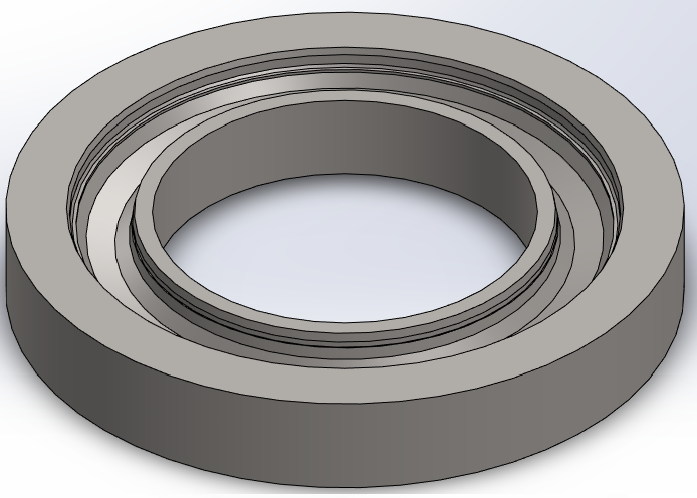
\includegraphics[width = 0.9\textwidth]{Figures/Cap3/CAD_DB35.png}
        \caption{}
        \label{fig:CAD_DB35}
    \end{subfigure}%
    \centering
    \begin{subfigure}{.33\textwidth}
        \centering
        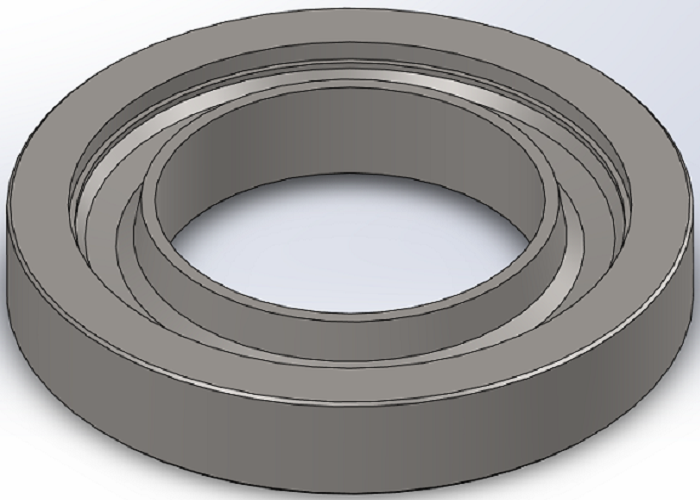
\includegraphics[width = 0.9\textwidth]{Figures/Cap3/CAD_DB45.png}
        \caption{}
        \label{fig:CAD_DB45}
    \end{subfigure}
    \centering
    \begin{subfigure}{.33\textwidth}
        \centering
        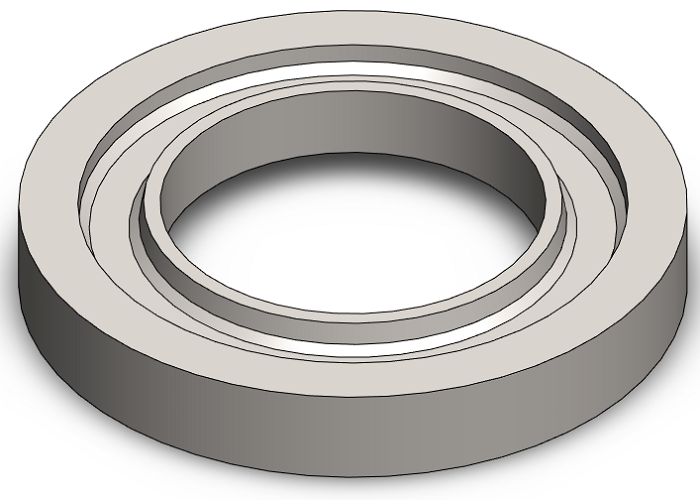
\includegraphics[width = 0.9\textwidth]{Figures/Cap3/CAD_JT4.png}
        \caption{}
        \label{fig:CAD_JT4}
    \end{subfigure}
    \centering
    \begin{subfigure}{.33\textwidth}\
        \centering
        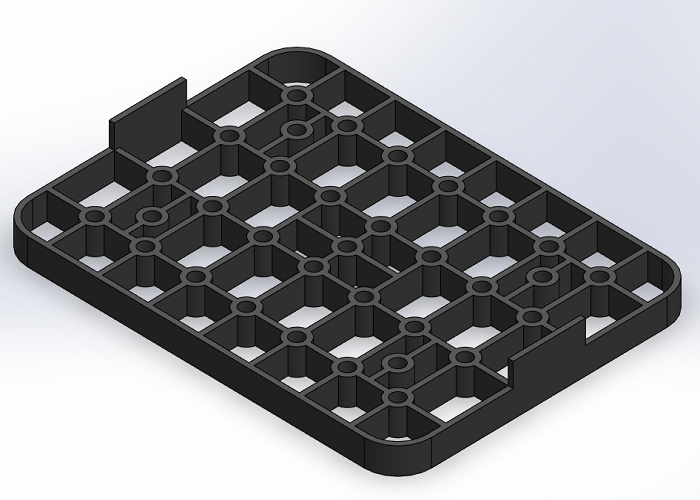
\includegraphics[width = 0.9\textwidth]{Figures/Cap3/CAD_PRATO.png}
        \caption{}
        \label{fig:CAD_Prato}
    \end{subfigure}%
    \centering
    \begin{subfigure}{.33\textwidth}
        \centering
        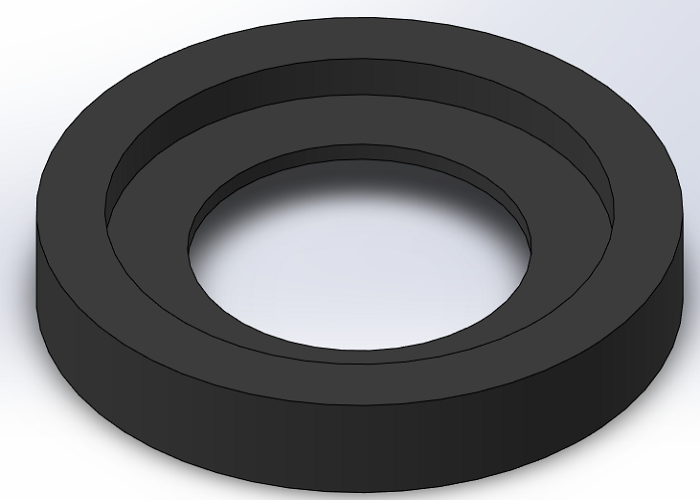
\includegraphics[width = 0.9\textwidth]{Figures/Cap3/CAD_FALSA.png}
        \caption{}
        \label{fig:CAD_Falsa}
    \end{subfigure}
    \centering
    \begin{subfigure}{.33\textwidth}
        \centering
        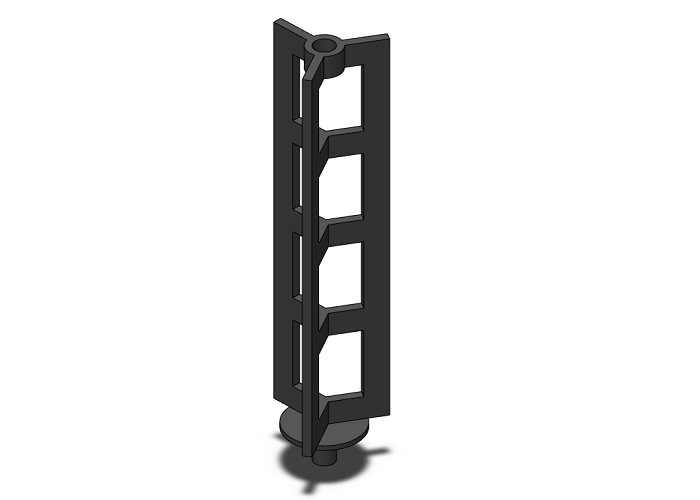
\includegraphics[width = 0.9\textwidth]{Figures/Cap3/CAD_TORRE.png}
        \caption{}
        \label{fig:CAD_Torre}
    \end{subfigure}
    \caption[Modelos 3D das rodas de coroa e dos elementos da ferramenta porta-peças.]%
    {\textbf{(a)} Modelo CAD 3D de uma roda de coroa DB35; \textbf{(b)} Modelo de uma roda de coroa DB45; \textbf{(c)} Modelo de uma roda de coroa JT4; \textbf{(d)} Modelo de um prato da ferramenta porta-peças; \textbf{(e)} Modelo de uma falsa coroa da ferramenta porta-peças; \textbf{(a)} Modelo de uma torre da ferramenta porta-peças.}
\end{figure}
%%%%%%%%%%%%%%%%%%%%%%%%%%%%%%%%%%%%%%%%%%%%%%%%%%%%%%%%%%%%%%%%%%%%%%%%%%%%%
% \par
% Após todos os elementos do sistema estarem modelados, realizou-se a montagem do sistema a ser simulado. Basicamente, como no porta-peças real, cada prato contêm 5 torres, e cada torre contem 10 rodas de coroa, no caso da DB45 e 11 rodas de coroa, no caso da DB35 e JT4.
%%%%%%%%%%%%%%%%%%%%%%%%%%%%%%%%%%%%%%%%%%%%%%%%%%%%%%%%%%%%%%%%%%%%%%%%%%%%%
\begin{table}[htb]
    \centering
    \caption[Propriedades mecânicas e térmicas do aço 27MC5]%
    {Propriedades mecânicas e térmicas do aço 27MC5 usadas nas simulações CFD.}
    \label{tab:Propriedades_27MC5}
    \begin{tabular}{lrr} 
    \toprule
    \multicolumn{1}{c}{\textbf{Propriedades}} & \multicolumn{1}{c}{\textbf{Aço 27MC5}}            & \multicolumn{1}{c}{\textbf{Refratário EN 1.4807}}  \\ 
    \hline\hline
    Densidade ($\rho$)                        & 7800 kg m\textsuperscript{-3}                     & 8000 kg m\textsuperscript{-3}                      \\
    Módulo de Young (E)                       & 190 GPa                                           & 190 GPa                                            \\
    Coeficiente de poisson ($\nu$)            & 0,29                                              & 0,29                                               \\
    Tensão de limite elástico (\textit{T})             & 380 MPa                                           & 120 MPa                                            \\
    Coef. de expansão térmica (\textit{a})             & 0,13 $\mu$K\textsuperscript{-1}                   & 0,15 $\mu$K\textsuperscript{-1}                    \\
    Coef. de condutividade térmica (\textit{K})        & 46 W m\textsuperscript{-1}K\textsuperscript{-1}   & 12 W m\textsuperscript{-1}K\textsuperscript{-1}    \\
    Calor específico (\textit{c})                      & 470 J kg\textsuperscript{-1}K\textsuperscript{-1} & 480 J kg\textsuperscript{-1}K\textsuperscript{-1}  \\
    \toprule
    \end{tabular}
    \end{table}
%%%%%%%%%%%%%%%%%%%%%%%%%%%%%%%%%%%%%%%%%%%%%%%%%%%%%%%%%%%%%%%%%%%%%%%%%%%%%
\newpage
\par
Uma vez que o modelo CFD necessita de alguns dados dos materiais e do fluido térmico, estes podem ser encontrados nas Tabelas \ref{tab:Propriedades_27MC5} e \ref{tab:Propriedades_VolutaH300}, e uma imagem do modelo montado pode ser vista na Figura \ref{fig:modelo_montado}
%%%%%%%%%%%%%%%%%%%%%%%%%%%%%%%%%%%%%%%%%%%%%%%%%%%%%%%%%%%%%%%%%%%%%%%%%%%%%
\begin{table}[htb]
    \centering
    \caption[Propriedades do fluido de têmpera Voluta H300]%
    {Propriedades mecânicas e térmicas do aço 27MC5 usadas nas simulações CFD.}
    \label{tab:Propriedades_VolutaH300}
    \begin{tabular}{lrrr} 
    \toprule
    \multicolumn{1}{c}{\textbf{Propriedades Voluta H300}} & \multicolumn{1}{c}{\textbf{20 °C}} & \multicolumn{1}{c}{\textbf{100 °C}} & \multicolumn{1}{c}{\textbf{140 °C}}  \\ 
    \hline\hline
    Densidade ($\rho$)                                    & 780 kg m\textsuperscript{-3}       & 600 kg m\textsuperscript{-3}        & 600 kg m\textsuperscript{-3}         \\
    Viscosidade cinemática ($\mu$)                        & 571 cSt                            & 190 cSt                             & 4,8 cSt                              \\
    Temperatura de transf. de fase (\textit{T})           & \multicolumn{3}{c}{400 °C}                                                                                      \\
    Coef. de condutividade térmica (\textit{K})           & \multicolumn{3}{c}{46 W m\textsuperscript{-1}K\textsuperscript{-1}}                                             \\
    Calor específico (\textit{cp})                        & \multicolumn{3}{c}{470 J kg\textsuperscript{-1}K\textsuperscript{-1}}                                           \\
    \bottomrule
    \end{tabular}
    \end{table}
%%%%%%%%%%%%%%%%%%%%%%%%%%%%%%%%%%%%%%%%%%%%%%%%%%%%%%%%%%%%%%%%%%%%%%%%%%%%%
%%%%%%%%%%%%%%%%%%%%%%%%%%%%%%%%%%%%%%%%%%%%%%%%%%%%%%%%%%%%%%%%%%%%%%%%%%%%%
\begin{figure}[htb]
    \centering
    \begin{subfigure}{.5\textwidth}\
        \centering
        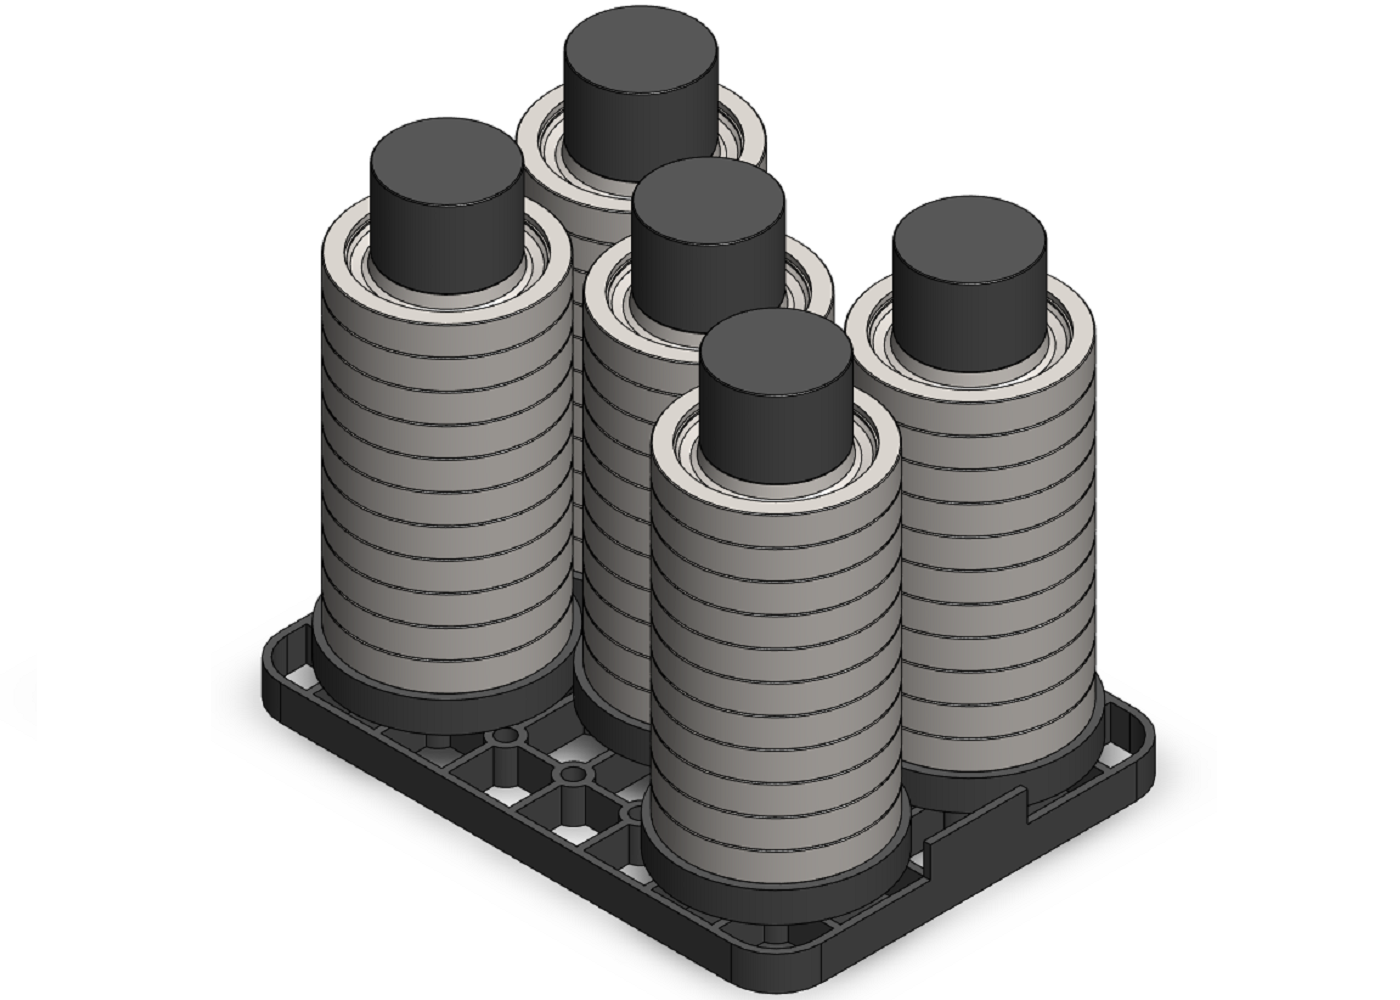
\includegraphics[width = 0.9\textwidth]{Figures/Cap3/Prato_montado.png}
        \caption{}
        \label{fig:modelo_montado}
    \end{subfigure}%
    \begin{subfigure}{.5\textwidth}
        \centering
        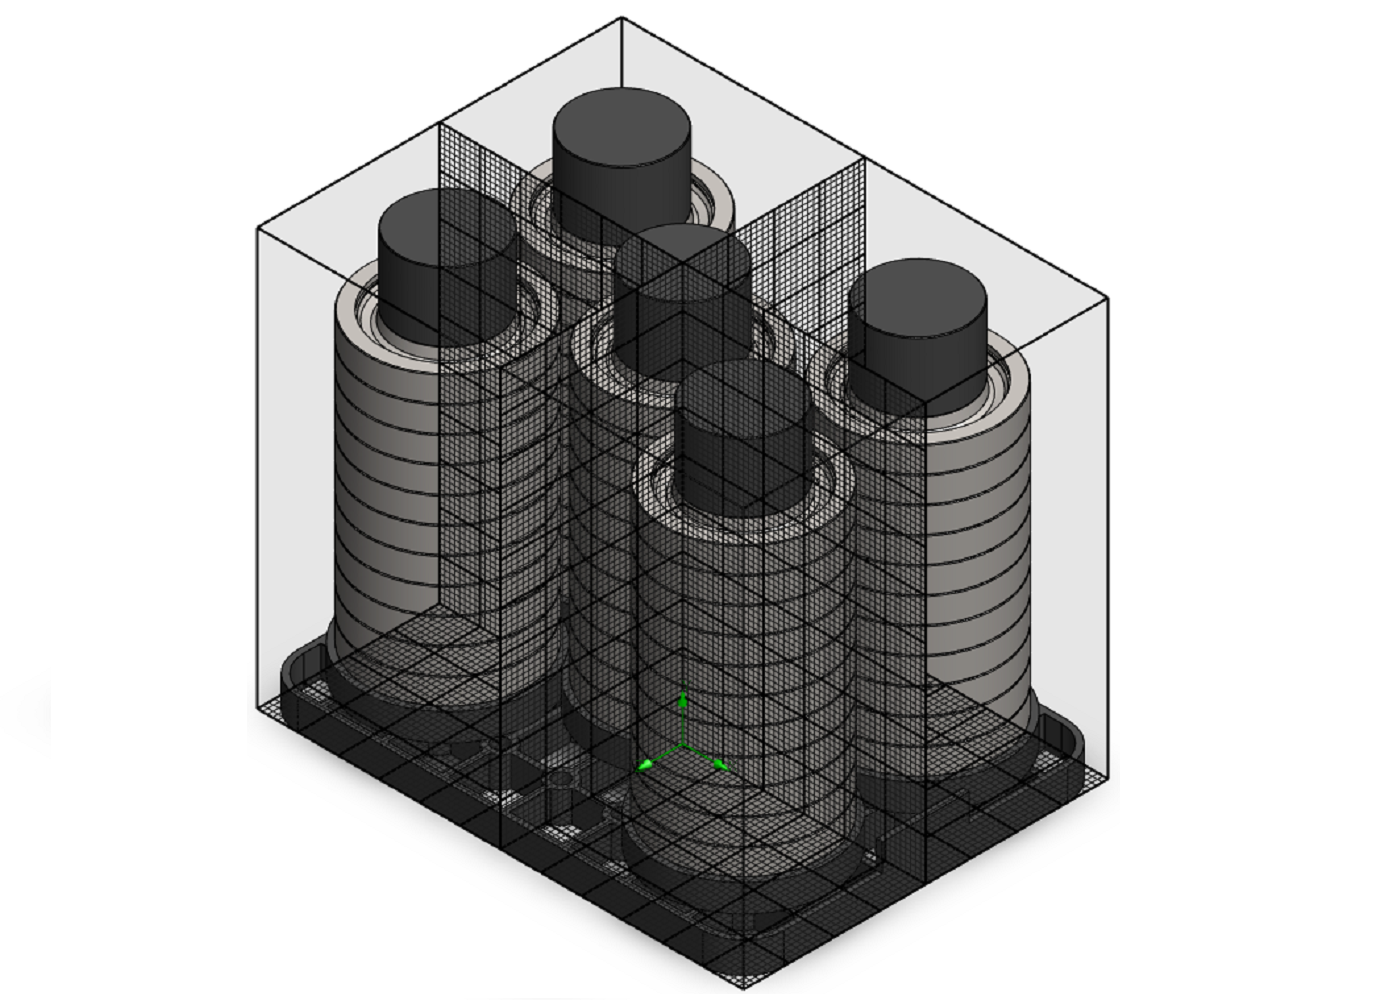
\includegraphics[width = 0.9\textwidth]{Figures/Cap3/Prato_montado_malha.png}
        \caption{}
        \label{fig:malha_simulacao}
    \end{subfigure}
    \caption[Modelo 3D de um prato montado e esquema de malhas da simulação.]%
    {À esquerda, modelo CAD 3D de um prato de rodas de coroa DB45 montado. À direita, esquema de malhas utilizado na simulação CFD.}
\end{figure}
%%%%%%%%%%%%%%%%%%%%%%%%%%%%%%%%%%%%%%%%%%%%%%%%%%%%%%%%%%%%%%%%%%%%%%%%%%%%%
\par
Por fim, utiliza-se o add-on \textit{Flow Simulation} do software SolidWorks para criar um programa de simulações, de forma a visualizar o comportamento do fluido de têmpera nas condições de tratamento. Para além dos dados indicados nas tabelas acima, às peças foi definida uma temperatura de 870 \textdegree C, e foram utilizados um coeficiente de rugosidade em todas as faces das rodas de coroa de 50$\mu$m, uma rugosidade de 500 $\mu$m em todas as faces dos componentes da ferramenta porta-peças, e foi definida uma malha “grosseira” para os elementos sólidos, e uma malha “normal” para os elementos de fluido. Ver Figura \ref{fig:malha_simulacao}.
\par
Os limites computacionais do fluido foram definidos de acordo com as dimensões do tanque que encontra-se descrito na Figura \ref{fig:tanque_tempera}, ou seja, (700x700) mm\textsuperscript{2} de base e 900 mm de altura, e o plano inferior do tanque foi assumido como uma entrada uniforme de fluido de tempera a uma velocidade de 1,45 m/s, e a uma temperatura de 170 \textdegree C de acordo com o documento do tanque que pode ser visualizado no Apêndice \ref{ap:tanque_tempera}.
\newpage
\par
Uma vez que, mesmo com geometrias pouco complexas e com a utilização de uma malha “grosseira” nos elementos sólidos, a simulação em questão tem um grande custo computacional, esta consumiu cerca de 9 horas até estar completa, e com isto, como pode ser visto na Figura \ref{fig:resultado_serie}, é possível  que o fluxo de fluido é tão grande ou talvez até mais volumoso no diâmetro interno das rodas de coroa que no dentado, portanto, confirmando mais uma vez que é realizada uma têmpera no diâmetro interno da mesma maneira que no dentado. No entanto, não há necessidade da existência de grandes durezas no diâmetro interno, e a presença de martensite é indesejada, por conta da ocorrência de fissurações a hidrogénio.
% \par
% Dito isso, confirma-se a necessidade da conceção de um sistema de tamponamento para evitar o fluxo de fluido térmico por este diâmetro, ao adicionar uma “tampa” simples, e soldar a coluna á falsa coroa, criando assim uma “geometria protegida” contra a têmpera.
%%%%%%%%%%%%%%%%%%%%%%%%%%%%%%%%%%%%%%%%%%%%%%%%%%%%%%%%%%%%%%%%%%%%%%%%%%%%%
\begin{figure}[htb]
    \centering
    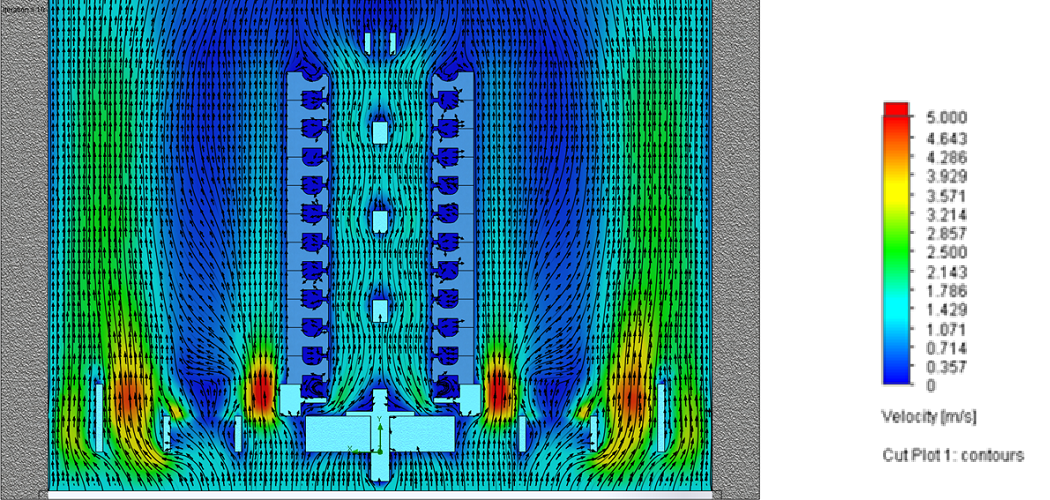
\includegraphics[width = 0.8\textwidth]{Figures/Cap3/resultado_serie.png}
    \caption[Resultado da simulação CFD da têmpera das rodas de coroa de série]%
    {Imagem de um corte no plano XZ, a meio da coluna central, do fluxo de fluido resultante da imersão do prato de rodas de coroa DB45 de série no tanque de têmpera, onde o gradiente de cores corresponde à velocidade do fluido, com \colorbox{Blue}{\textcolor{White}{azul escuro sendo 0 m/s}}, e \colorbox{Red}{\textcolor{White}{vermelho sendo 5 m/s ou maior.}}}
    \label{fig:resultado_serie}
\end{figure}
%%%%%%%%%%%%%%%%%%%%%%%%%%%%%%%%%%%%%%%%%%%%%%%%%%%%%%%%%%%%%%%%%%%%%%%%%%%%%
\subsection{Simulação da tampa simples}  \label{ssec:materiais_concecao_simples}
Como visto ser necessário na subsecção anterior, foi desenvolvida uma nova ferramenta porta-peças para proteger o diâmetro interno, com uma tampa na parte superior (Ver Figura \ref{fig:tampa_simples}), e onde se aproveitou a falsa coroa, a torre e o prato, foi adicionado um copo para permitir a soldadura da torre na falsa coroa (Ver \ref{fig:falsa_coroa_torre}). A imagem da ferramenta porta-peças e uma vista em corte, com uma coluna de rodas de coroa DB45 montada pode ser vista nas Figuras \ref{fig:simples_montada}, e \ref{fig:simples_corte}, respetivamente.

%%%%%%%%%%%%%%%%%%%%%%%%%%%%%%%%%%%%%%%%%%%%%%%%%%%%%%%%%%%%%%%%%%%%%%%%%%%%%
\begin{figure}[htb]
    \centering
    \begin{subfigure}{.5\textwidth}\
        \centering
        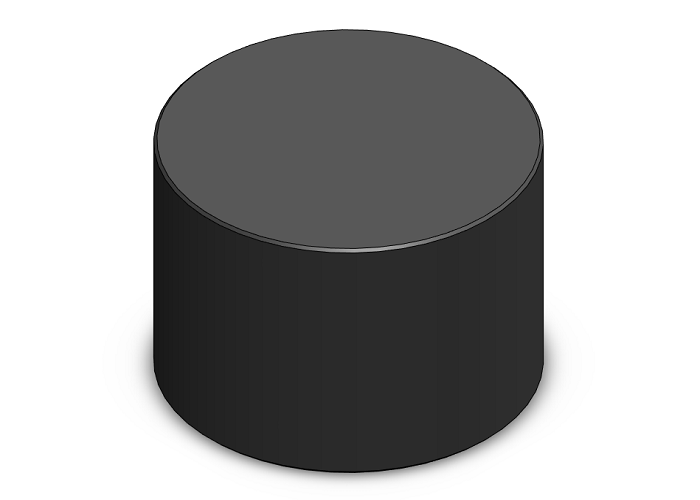
\includegraphics[width = 0.5\textwidth]{Figures/Cap3/Tampa_P.png}
        \caption{}
        \label{fig:tampa_simples}
    \end{subfigure}%
    \begin{subfigure}{.5\textwidth}
        \centering
        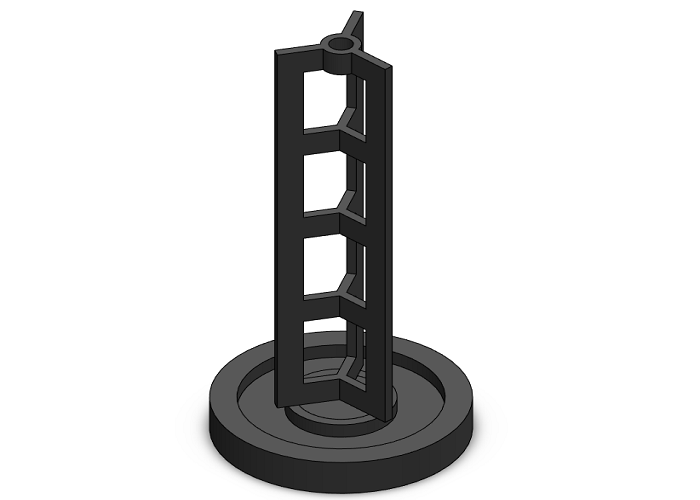
\includegraphics[width = 0.5\textwidth]{Figures/Cap3/Falsa_coroa_modificada.png}
        \caption{}
        \label{fig:falsa_coroa_torre}
    \end{subfigure}
    \caption[Imagens ilustrativas dos componentes modificados da proposta inicial.]%
    {Imagens ilustrativas em CAD 3D dos sistemas que compõem a proposta inicial da ferramenta porta-peças com diâmetro protegido.}
\end{figure}
%%%%%%%%%%%%%%%%%%%%%%%%%%%%%%%%%%%%%%%%%%%%%%%%%%%%%%%%%%%%%%%%%%%%%%%%%%%%%
\newpage
%%%%%%%%%%%%%%%%%%%%%%%%%%%%%%%%%%%%%%%%%%%%%%%%%%%%%%%%%%%%%%%%%%%%%%%%%%%%%
\begin{figure}[htb]
    \centering
    \begin{subfigure}{.5\textwidth}\
        \centering
        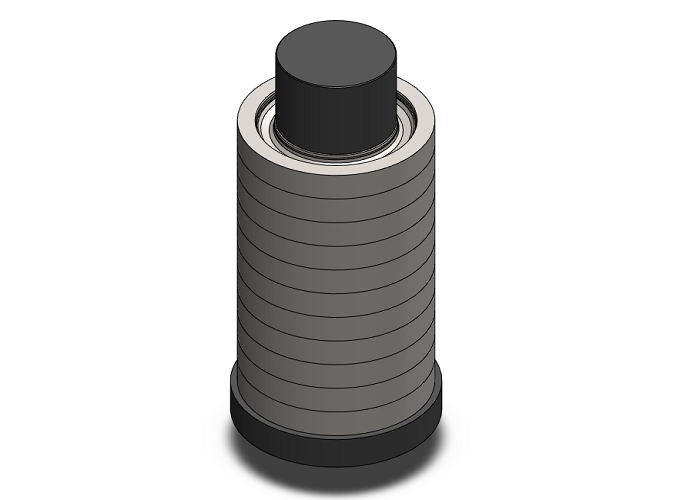
\includegraphics[width = 0.7\textwidth]{Figures/Cap3/Coluna_P_Montada.png}
        \caption{}
        \label{fig:simples_montada}
    \end{subfigure}%
    \begin{subfigure}{.5\textwidth}
        \centering
        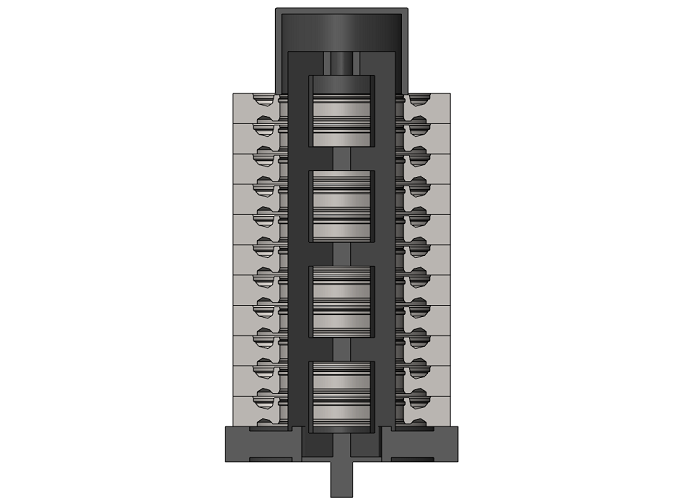
\includegraphics[width = 0.7\textwidth]{Figures/Cap3/Coluna_P_Montada_Corte.png}
        \caption{}
        \label{fig:simples_corte}
    \end{subfigure}
    \caption[Imagens ilustrativas da proposta inicial montada e em corte.]%
    {Imagens ilustrativas em CAD 3D do sistema montado com uma coluna de rodas de coroa DB45 em vista isométrica e em vista frontal em corte.}
\end{figure}
%%%%%%%%%%%%%%%%%%%%%%%%%%%%%%%%%%%%%%%%%%%%%%%%%%%%%%%%%%%%%%%%%%%%%%%%%%%%%
\par
Tendo o modelo CAD da ferramenta, fez-se então uma simulação nos mesmos parâmetros definidos para o sistema de série, podendo o resultado do fluxo de fluido térmico ser observado na Figura \ref{fig:resultado_simples}. Como é possível observar, o fluxo de fluido térmico é um pouco afetado no dentado das rodas de coroa inferiores, no entanto, não há quase nenhum fluxo de fluido térmico dentro da geometria que se deseja proteger, o que indica que provavelmente haverá pouca ou nenhuma têmpera nos diâmetros internos das rodas de coroa com este tipo de ferramenta porta-peças.
%%%%%%%%%%%%%%%%%%%%%%%%%%%%%%%%%%%%%%%%%%%%%%%%%%%%%%%%%%%%%%%%%%%%%%%%%%%%%
\begin{figure}[htb]
    \centering
    \includegraphics[width = 0.8\textwidth]{Figures/Cap3/resultado_simples.png}
    \caption[Resultado da simulação CFD da têmpera das rodas de coroa com diâmetro protegido]%
    {Imagem de um corte no plano XZ, a meio da coluna central, do fluxo de fluido resultante da imersão do prato de rodas de coroa DB45 com diâmetro protegido no tanque de têmpera, onde o gradiente de cores corresponde à velocidade do fluido, com \colorbox{Blue}{\textcolor{White}{azul escuro sendo 0 m/s}}, e \colorbox{Red}{\textcolor{White}{vermelho sendo 5 m/s ou maior.}}}
    \label{fig:resultado_simples}
\end{figure}
%%%%%%%%%%%%%%%%%%%%%%%%%%%%%%%%%%%%%%%%%%%%%%%%%%%%%%%%%%%%%%%%%%%%%%%%%%%%%
\newpage
\subsection{Prototipagem da tampa simples}  \label{ssec:materiais_prototipagem_simples}
Tendo então resultados satisfatórios na simulação, prosseguiu-se com a próxima etapa da conceção da ferramenta. Para verificar que as dimensões geométricas estavam compatíveis com os sistemas produtivos, fez-se uma impressão 3D dos componentes modificados que podem ser vistos nas Figuras \ref{fig:Tampa_simples_3d}, \ref{fig:falsa_coroa_torre_3d}. Estes componentes tiveram suas dimensões verificadas num prato de rodas de coroa de série DB45. Verificadas as dimensões, como pode ser visto na Figura \ref{fig:teste_impressao_3d}, prosseguiu-se com a ordem de trabalho para maquinar uma tampa simples e modificar a torre e a falsa coroa, de forma a realizar um ensaio de tratamento térmico, para verificar a microestrutura e as durezas e comparar os resultados com as rodas de coroa de série.
%%%%%%%%%%%%%%%%%%%%%%%%%%%%%%%%%%%%%%%%%%%%%%%%%%%%%%%%%%%%%%%%%%%%%%%%%%%%%
\begin{figure}[htb]
    \centering
    \begin{subfigure}{.5\textwidth}\
        \centering
        \includegraphics[width = 0.9\textwidth]{Figures/Cap3/tampa_simples_3d.png}
        \caption{}
        \label{fig:Tampa_simples_3d}
    \end{subfigure}%
    \begin{subfigure}{.5\textwidth}
        \centering
        \includegraphics[width = 0.9\textwidth]{Figures/Cap3/Falsa_coroa_torre_3d.png}
        \caption{}
        \label{fig:falsa_coroa_torre_3d}
    \end{subfigure}
    \caption[Modelos dos componentes modificados impressos em PET-G.]%
    {Modelos impressos em PET-G no laboratório de impressão 3D da Renault Cacia, Á direita a tampa simples e à esquerda, a falsa coroa soldada à torre. Toda a impressão foi feita durante o fim de semana e durou mais de 40 horas.}
\end{figure}
%%%%%%%%%%%%%%%%%%%%%%%%%%%%%%%%%%%%%%%%%%%%%%%%%%%%%%%%%%%%%%%%%%%%%%%%%%%%%
%%%%%%%%%%%%%%%%%%%%%%%%%%%%%%%%%%%%%%%%%%%%%%%%%%%%%%%%%%%%%%%%%%%%%%%%%%%%%
\begin{figure}[htb]
    \centering
    \includegraphics[width = 0.9\textwidth]{Figures/Cap3/Teste_impressao_largo.png}
    \caption[Teste dos componentes impressos em 3D no prato e nas rodas de coroa]%
    {Fotografia do teste dos componentes impressos em 3D no prato e nas rodas de coroa, para verificar se as dimensões projetadas são compatíveis com os componentes já existentes.}
    \label{fig:teste_impressao_3d}
\end{figure}
%%%%%%%%%%%%%%%%%%%%%%%%%%%%%%%%%%%%%%%%%%%%%%%%%%%%%%%%%%%%%%%%%%%%%%%%%%%%%
\newpage
%%%%%%%%%%%%%%%%%%%%%%%%%%%%%%%%%%%%%%%%%%%%%%%%%%%%%%%%%%%%%%%%%%%%%%%%%%%%%
\subsection{Ensaio da proposta inicial} \label{ssec:materiais_ensaio_simples}
Como referido na subsecção anterior, foi realizado um ensaio da ferramenta modificada, onde o objetivo era verificar se os resultados obtidos pela simulação CFD eram condizentes com a realidade, para isto, separou-se uma carga montada com 150 rodas de coroa DB45, onde de um dos pratos, substituindo uma das colunas de rodas de coroa com a ferramenta modificada, como pode ser visto na Figura \ref{fig:ensaio_simples}. Também pode ser visto na Figura \ref{fig:esquema_ensaio_simples}, um desenho esquemático que orienta a disposição da ferramenta modificada num dos pratos. Para além disso, a carga modificada seguiu com um aviso escrito em papel, um aviso por e-mail e um aviso verbal, da forma que se deveria realizar o ensaio, ou seja, que as peças estavam identificadas de 1 a 10, onde 1 seria a roda de coroa mais em baixo, e 10 a roda de coroa mais em cima, que a carga poderia ser identificada pela presença de uma tampa na coluna central do primeiro prato e que, após o revenido, as peças não deveriam seguir para a granalhagem, e que deveriam ser separadas para serem levadas ao laboratório de ensaios mecânicos.
%%%%%%%%%%%%%%%%%%%%%%%%%%%%%%%%%%%%%%%%%%%%%%%%%%%%%%%%%%%%%%%%%%%%%%%%%%%%%
\begin{figure}[htb]
    \centering
    \includegraphics[width = 0.5\textwidth]{Figures/Cap3/Ensaio_simples.png}
    \caption[Montagem do ensaio do protótipo inicial da ferramenta modificada]%
    {Fotografia da montagem da ferramenta porta-peças modificada para o ensaio inicial da proteção do diâmetro.}
    \label{fig:ensaio_simples}
\end{figure}
%%%%%%%%%%%%%%%%%%%%%%%%%%%%%%%%%%%%%%%%%%%%%%%%%%%%%%%%%%%%%%%%%%%%%%%%%%%%%
%%%%%%%%%%%%%%%%%%%%%%%%%%%%%%%%%%%%%%%%%%%%%%%%%%%%%%%%%%%%%%%%%%%%%%%%%%%%%
\begin{figure}[htb!]
    \centering
    \includegraphics[width = 0.5\textwidth]{Figures/Cap3/Desenho_ensaio_simples.png}
    \caption[Desenho do esquema de montagem da ferramenta]%
    {Desenho feito em SolidWorks do esquema que foi montado o primeiro prato da carga de ensaio, onde a ferramenta modificada encontra-se no centro do primeiro prato da carga.}
    \label{fig:esquema_ensaio_simples}
\end{figure}
%%%%%%%%%%%%%%%%%%%%%%%%%%%%%%%%%%%%%%%%%%%%%%%%%%%%%%%%%%%%%%%%%%%%%%%%%%%%%
\newpage
\par
Para a realização das medições de dureza no Laboratório de Ensaios Mecânicos (LEMM) foram removidas as rodas de coroa de baixo, ou Nº 1, do meio, ou Nº 6 e de cima, ou Nº 10. Foram feitas filiações das duas zonas de soldadura do diferencial, denominadas por “Zona 1” e “Zona 2”; das duas zonas de prensagem, denominadas por “Zona 3” e “Zona 4”; das duas zonas de soldadura da “Cible”, denominadas por “Zona Cible 1” e “Zona Cible 2”; tres picagens nas zonas do dentado; e a dureza superficial, medida em HRC. A Figura \ref{fig:zonas_filiacoes_dureza} ilustra, num desenho de uma roda de coroa DB45, a posição das zonas das filiações de dureza.
%%%%%%%%%%%%%%%%%%%%%%%%%%%%%%%%%%%%%%%%%%%%%%%%%%%%%%%%%%%%%%%%%%%%%%%%%%%%%
\begin{figure}[htb!]
    \centering
    \includegraphics[width = 0.5\textwidth]{Figures/Cap3/Zonas_dureza.png}
    \caption[Zonas das filiações de dureza]%
    {Desenho indicativo das zonas onde são feitas as filiações de dureza das rodas de coroa, de forma a verificar se a proteção do diâmetro interno é efetiva e que nao há alterações nos valores de dureza do dentado.}
    \label{fig:zonas_filiacoes_dureza}
\end{figure}
%%%%%%%%%%%%%%%%%%%%%%%%%%%%%%%%%%%%%%%%%%%%%%%%%%%%%%%%%%%%%%%%%%%%%%%%%%%%%
\par
Os resultados destas filiações de dureza serão discutidos no Capítulo \ref{ch:resultados}, no entanto, para efeitos da continuidade do trabalho, é necessário dizer que, mesmo que os resultados tenham sido satisfatórios, os valores das durezas em todas as zonas nas rodas de coroa inferiores foram consideravelmente superiores aos valores nas rodas de coroa do meio e de cima. Além disso, na roda de coroa Nº 10, a dureza na zona de soldadura da Cible não foi afetada pela proteção, além da “zona 1” ter durezas ligeiramente superiores às durezas na mesma zona nas outras rodas de coroa, o que leva à suspeita de que a existência de uma aba seria necessária para uniformizar os valores de durezas em todas as 10 rodas de coroa da coluna. Por fim, verificou-se que a soldadura feita na falsa coroa à torre da ferramenta porta-peças sofreu rotura, o que também pode explicar o motivo das durezas em todas as zonas da roda de coroa Nº 1 serem muito maiores que as demais.
%%%%%%%%%%%%%%%%%%%%%%%%%%%%%%%%%%%%%%%%%%%%%%%%%%%%%%%%%%%%%%%%%%%%%%%%%%%%%
\subsection{Novos protótipos e melhorias} \label{ssec:novos_prototipos}
Devido aos problemas encontrados no ensaio do protótipo inicial, foram desenvolvidos dois outros protótipos. O primeiro, denominado “Tampa O” sendo uma modificação do protótipo inicial, apenas com a adição de uma aba de proteção para a cible. O segundo, alterando a geometria de um “copo” para um formato ajustado à torre da ferramenta porta-peças das peças de série, denominado “Tampa Y”. A Figura \ref{fig:novos_prototipos} ilustra as geometrias novas. A ferramenta inicial foi então denominada “Tampa P”, em homenagem ao “Engenheiro Pinto” responsável pela sua geometria e pela ideia de proteger o diâmetro interno das rodas de coroa quanto à Têmpera.
%%%%%%%%%%%%%%%%%%%%%%%%%%%%%%%%%%%%%%%%%%%%%%%%%%%%%%%%%%%%%%%%%%%%%%%%%%%%%
\begin{figure}[htb]
    \centering
    \begin{subfigure}{.5\textwidth}\
        \centering
        \includegraphics[width = 0.9\textwidth]{Figures/Cap3/Tampa_O.png}
        \caption{}  
    \end{subfigure}%
    \begin{subfigure}{.5\textwidth}
        \centering
        \includegraphics[width = 0.9\textwidth]{Figures/Cap3/Tampa_Y.png}
        \caption{}
    \end{subfigure}
    \caption[Modelos CAD dos novos protótipos de tampa]%
    {Modelos em CAD 3D dos novos protótipos que buscam melhorar os parâmetros resultantes do ensaio com a ferramenta inicial. À direita a “Tampa O” e à esquerda a “Tampa Y”.}
    \label{fig:novos_prototipos}
\end{figure}
%%%%%%%%%%%%%%%%%%%%%%%%%%%%%%%%%%%%%%%%%%%%%%%%%%%%%%%%%%%%%%%%%%%%%%%%%%%%%
\newpage
\par
Além da modificação das tampas, também foi modificada a junção da falsa coroa com a torre, uma vez que no protótipo inicial foi realizada uma soldadura muito simples, com apenas três “pingos” de soldadura em todo o diâmetro, desta vez, foi feita uma soldadura completa, em toda o diâmetro. Sendo as suspeitas de que os resultados do ensaio inicial foram afetados pela rotura da soldadura verdade, os próximos ensaios devem conferir resultados mais uniformes em todas as rodas de coroa da coluna tratada. Por fim, um novo protótipo foi testado para verificar a necessidade da utilização de uma tampa, sendo assim o próximo ensaio constituído por 5 colunas completas; uma coluna protegida pela tampa Y; uma coluna protegida pela tampa O; uma coluna protegida pela tampa P; uma coluna protegida apenas pela falsa coroa modificada, em baixo; e uma coluna sem proteção alguma, denominada coluna de série. Um desenho com o esquema de configuração deste prato para ensaio pode ser visto na Figura \ref{fig:configuracao_ensaio}.
%%%%%%%%%%%%%%%%%%%%%%%%%%%%%%%%%%%%%%%%%%%%%%%%%%%%%%%%%%%%%%%%%%%%%%%%%%%%%
\begin{figure}[htb!]
    \centering
    \begin{subfigure}{.5\textwidth}\
        \centering
        \includegraphics[width = 0.9\textwidth]{Figures/Cap3/Esquema_Prato_Ensaio_08-05-2023.png}
        \caption{}  
    \end{subfigure}%
    \begin{subfigure}{.5\textwidth}\
        \centering
        \includegraphics[width = 0.9\textwidth]{Figures/Cap3/Ensaio_varias_tampas.png}
        \caption{}  
    \end{subfigure}%
    \caption[Configuração do ensaio dos vários protótipos]%
    {à esquerda, um desenho indicativo da configuração das ferramentas num prato para realização do ensaio com os vários protótipos. À direita, uma fotografia da carga montada para ensaio.}
    \label{fig:configuracao_ensaio}
\end{figure}
%%%%%%%%%%%%%%%%%%%%%%%%%%%%%%%%%%%%%%%%%%%%%%%%%%%%%%%%%%%%%%%%%%%%%%%%%%%%%
\newpage
\par
Para a execução deste ensaio, foi necessário proceder à marcação das rodas de coroa, não só numa sequência numérica de 1 a 10, mas também numa sequência alfabética. Neste sistema, as rodas de coroa designadas por “A” correspondem à tampa Y, as “B” à tampa O, as “C” à tampa P, as “D” à coluna sem tampa, e as “S” à coluna de série. Assim, a roda de coroa marcada como “B10” representa, por exemplo, a roda de coroa no topo da coluna protegida pela tampa O. No ensaio anterior, surgiu um problema no reconhecimento das peças à entrada do forno de revenido, uma vez que o sistema se baseia na imagem do perfil do diâmetro da peça central, e as tampas não são identificadas automaticamente. Para contornar esta questão, optou-se por remover as tampas após a primeira máquina de lavar, tendo em conta que, caso fossem removidas após a têmpera, as tampas estariam a uma temperatura de 170\textdegree C, demasiado quente para uma manipulação segura.
\par
Paralelamente a este ensaio, realizou-se um segundo, com as mesmas configurações, mas desta vez utilizando rodas de coroa JT4. Foram adicionados dois provetes do material 27MC5, um no interior da coluna com geometria protegida pela tampa Y e outro no interior da coluna de série. Estes provetes foram posteriormente enviados para um laboratório em França, onde se procedeu à realização de uma espectroscopia de emissão ótica de descarga luminescente. Este ensaio tem como objetivo aferir a composição dos materiais constituintes no provete, em particular, verificar a ocorrência de enriquecimento de carbono e azoto no diâmetro interno das rodas de coroa protegidas no forno de carbonitruração, e comparar os resultados com o enriquecimento observado nas rodas de coroa de série. Um esquema do ensaio e a posição dos provetes estão ilustrados na Figura \ref{fig:ensaio_gales}. Uma fotografia de um provete antes do ensaio pode ser observada na Figura \ref{fig:gales}.
%%%%%%%%%%%%%%%%%%%%%%%%%%%%%%%%%%%%%%%%%%%%%%%%%%%%%%%%%%%%%%%%%%%%%%%%%%%%%
\begin{figure}[htb!]
    \centering
    \begin{subfigure}{.5\textwidth}\
        \centering
        \includegraphics[width = 0.9\textwidth]{Figures/Cap3/Layout_ensaio_gallets.png}
        \caption{}
        \label{fig:ensaio_gales}  
    \end{subfigure}%
    \begin{subfigure}{.5\textwidth}\
        \centering
        \includegraphics[width = 0.9\textwidth]{Figures/Cap3/Gallets.png}
        \caption{}
        \label{fig:gales}  
    \end{subfigure}%
    \caption[Configuração do ensaio dos vários protótipos]%
    {à esquerda, desenho indicativo da configuração das ferramentas num prato para realização do ensaio com os vários protótipos. Esta configuração é idêntica ao ensaio anterior, com a adição de duas galés, uma por dentro da coluna protegida por tampa Y, e uma por dentro da coluna de série. À direita, fotografia de uma das galés que foram inseridas na carga de ensaio.}
\end{figure}
%%%%%%%%%%%%%%%%%%%%%%%%%%%%%%%%%%%%%%%%%%%%%%%%%%%%%%%%%%%%%%%%%%%%%%%%%%%%%
\newpage
\par
Após este último, procedeu-se a um novo ensaio, desta vez com as rodas de coroa DB35, mantendo a mesma configuração dos ensaios anteriores realizados com as rodas de coroa DB45 e JT4. No entanto, tendo em conta que o tratamento e a recolha dos valores de dureza de cada ensaio demoram aproximadamente duas semanas para serem completados, à data da redação deste documento, os resultados ainda não estavam disponíveis. Consequentemente, o tratamento e a análise dos dados deste último ensaio não serão abordados no capítulo seguinte. Estava igualmente prevista a realização de um ensaio utilizando uma tinta "stop-off carbonitruração", bem como um ensaio no forno de revenido para a verificação do hidrogénio difusível. Infelizmente, devido ao escasso tempo disponível, estes ensaios não puderam ser realizados.
%%%%%%%%%%%%%%%%%%%%%%%%%%%%%%%%%%%%%%%%%%%%%%%%%%%%%%%%%%%%%%%%%%%%%%%%%%%%%
\subsection{Parâmetros de Conformidade e Metodologia de Ensaio} \label{ssec:parametros_metodologia}
Por fim, é importante elucidar o intervalo de parâmetros desejados para as rodas de coroa, bem como a metodologia de ensaio empregada para aferir tais parâmetros de conformidade. Importa ainda salientar que, caso estes parâmetros não sejam verificados na roda de coroa em teste, que nas rodas de coroa de série corresponde sempre à roda superior da coluna central do prato do meio de uma carga, toda a carga deve ser rejeitada e, por consequência, tratada como sucata. A Tabela \ref{tab:parametros_conformidade} apresenta os valores correspondentes aos diversos pontos, sendo estes os mesmos para todas as séries de roda de coroa, nomeadamente JT4, DB35 e DB45.
%%%%%%%%%%%%%%%%%%%%%%%%%%%%%%%%%%%%%%%%%%%%%%%%%%%%%%%%%%%%%%%%%%%%%%%%%%%%%
\begin{table}
    \centering
    \refstepcounter{table}
    \caption[Parâmetros de conformidade para rodas de coroa]%
    {Valores dos intervalos dos parâmetros de conformidade para rodas de coroa JT4, DB35 e DB45.}
    \label{tab:parametros_conformidade}
    \begin{tabular}{llr} 
    \toprule
    \multicolumn{1}{c}{\textbf{Etapa}} & \multicolumn{1}{c}{\textbf{Parâmetro de conformidade}} & \multicolumn{1}{c}{\textbf{Intervalo}}  \\ 
    \hline\hline
    \multirow{4}{*}{Peça Branca}       & Dentado sem riscos ou lascas                           & Sem defeito visual                      \\
                                       & Diâmetro externo                                       & 120,00 ± 0,04 mm                        \\
                                       & Diâmetro interno                                       & 80,00 ± 0,04 mm                         \\
                                       & Altura da peça                                         & 50,00 ± 0,04 mm                         \\ 
    \hline
    \multirow{4}{*}{Peça Negra}        & Dureza do dentado                                      & 680 a 900 HV                            \\
                                       & EC650                                                  & 0,6 a 0,8 mm                            \\
                                       & ET                                                     & 0,8 a 1,2 mm                            \\
                                       & Austenite residual                                     & Até 40\%                                \\
    \bottomrule
    \end{tabular}
\end{table}
%%%%%%%%%%%%%%%%%%%%%%%%%%%%%%%%%%%%%%%%%%%%%%%%%%%%%%%%%%%%%%%%%%%%%%%%%%%%%
    \chapter{Análise de Resultados} \label{ch:resultados}
\setlength{\headheight}{13.6pt}
%%%%%%%%%%%%%%%%%%%%%%%%%%%%%%%%%%%%%%%%%%%%%%%%%%%%%
Como referido no Capítulo \ref{ch:intro}, este capítulo é dedicado à exposição e análise dos resultados obtidos das simulações e experimentos realizados ao longo do projeto da ferramenta porta-peças desenvolvida.
\par
Uma vez que os resultados para as tres séries de rodas de coroa são similares, serão discutidos apenas resultados de uma série de rodas de coroa, para isto, foi selecionada a série DB45. A razão da escolha desta série de rodas de coroa não é outra além da disponibilidade dos resultados, uma vez que foi o primeiro ensaio a ser realizado, os resultados estavam disponíveis para serem tratados atempadamente. Pouco antes do final da redação deste documento, também estavam disponíveis os resultados das rodas de coroa de série JT4, e os resultados das rodas de coroa de série DB35 só estariam disponíveis após a data de entrega deste documento.
Para os resultados das simulações, foram necessários calcular as temperaturas de austenitização A\textsubscript{C1} e A\textsubscript{C3} do material, de acordo com as Equações \ref{eq:A_C1} e \ref{eq:A_C3}, respetivamente. A Tabela \ref{tab:temp_sim} indica estes valores, e outros valores importantes para a análise dos resultados das simulações que serão mostradas a seguir, na Secção \ref{sec:resultados_simulacoes}.
%%%%%%%%%%%%%%%%%%%%%%%%%%%%%%%%%%%%%%%%%%%%%%%%%%%%%%%%%%%%%%%%%%%%%%%%%%%%%

\begin{table}[htb]
    \centering
    \caption[Valores de temperatura importantes para a análise de resultados]%
    {Valores de temperaturas críticas, para o Aço 27MC5, antes e após a carbonitruração, respetivamente, importantes para a análise de resultados.}
    \label{tab:temp_sim}
    \begin{tabular}{lrr} 
    \toprule
    \textbf{Ponto Crítico}                  & \multicolumn{1}{c}{\textbf{Temperatura\textsubscript{Base}}} & \multicolumn{1}{c}{\textbf{Temperatura\textsubscript{(Carb.)}}}  \\ 
    \hline\hline
    Início de Austenitização \textbf{(A\textsubscript{C1})} & 707 °C                                            & 707 °C                                               \\
    Final de Austenitização \textbf{(A\textsubscript{C3})}  & 788 °C                                            & 715 °C                                               \\
    Início de Martensite \textbf{(M\textsubscript{S})}      & 370 °C                                            & 188 °C                                               \\
    Final de Martensite \textbf{(M\textsubscript{F})}       & 175 °C                                            & -30 °C                                               \\
    \hline
    Início de Têmpera \textbf{(T\textsubscript{0})}         & \multicolumn{2}{c}{870 °C}                                                                                \\
    Final de Têmpera \textbf{(T\textsubscript{F})}          & \multicolumn{2}{c}{170 °C}                                                                                \\
    \bottomrule
    \end{tabular}
    \end{table}
%%%%%%%%%%%%%%%%%%%%%%%%%%%%%%%%%%%%%%%%%%%%%%%%%%%%%%%%%%%%%%%%%%%%%%%%%%%%%
\newpage
\section{Resultados das simulações} \label{sec:resultados_simulacoes}
Alguns resultados das simulações já foram expostas no Capítulo \ref{ch:materiais} para efeitos de continuidade do documento, no entanto, alguns resultados necessitam ser analisados de forma a perceber as informações que podem ser adquiridas por simulação numérica.
\par
Como foi referido no passado capítulo, foi realizada uma simulação CFD de todos os protótipos desenvolvidos, entretanto, para além do esquema de velocidades do fluido de têmpera, é possível obter outros parâmetros de uma simulação CFD, entre estes, por exemplo, é possível obter os coeficientes de transferência de calor por convecção na interface entre os elementos finitos das rodas de coroa e os elementos finitos do fluido de têmpera, estes valores podem então ser inseridos numa simulação puramente térmica (Ver Figura \ref{fig:simulacao_termica}) onde é possível obter os valores das velocidades de arrefecimento nos vários pontos. Em especial, foram obtidos os valores da velocidade de arrefecimento num ponto do dentado e num ponto do diâmetro interno.
%%%%%%%%%%%%%%%%%%%%%%%%%%%%%%%%%%%%%%%%%%%%%%%%%%%%%%%%%%%%%%%%%%%%%%%%%%%%%
\begin{figure}[htb]
    \centering
    \includegraphics[width = 0.6\textwidth]{Figures/Cap4/Falta_Imagem.png}
    \caption[Simulação puramente térmica Solidworks]%
    {Add-in do Solidworks simulation thermal para uma simulação puramente térmica.}
    \label{fig:simulacao_termica}
\end{figure}
%%%%%%%%%%%%%%%%%%%%%%%%%%%%%%%%%%%%%%%%%%%%%%%%%%%%%%%%%%%%%%%%%%%%%%%%%%%%%
\par
Concluída a simulação, foram obtidos os valores do tempo em seis pontos, três para o dentado e três para o diâmetro interno. O primeiro ponto, é obtido quando os elementos atingem o valor de temperatura de austenitização A3, o segundo ponto, quando os elementos atingem a temperatura de austenitização A1, por fim, o terceiro ponto, quando os elementos atingem a temperatura de 170 \textdegree C. As Figuras \ref{fig:Dentado} são referentes aos pontos de temperaturas do dentado, e as Figuras \ref{fig:Diametro}
De forma a facilitar a visualização, nos resultados, as rodas de coroa são vistas pelo plano superior. Foram escolhidas sempre as rodas de coroa Nº 6, ou seja, as rodas do meio da coluna, e as simulações foram feitas num modelo CAD sem o dentado, com o objetivo de diminuir o número de elementos utilizados em cada simulação. A tabela \ref{tab:pontos_sim} indica os valores dos pontos e o tempo em cada um deles, que foram retirados das imagens. Com estes valores é então possível determinar a velocidade de arrefecimento nos pontos em questão e então estimar a microestrutura final no dentado e no diâmetro interno. Para além disso, é possível também prever a dureza final nos dois pontos, tendo em conta a microestrutura, a velocidade de arrefecimento e a composição química do material.
%%%%%%%%%%%%%%%%%%%%%%%%%%%%%%%%%%%%%%%%%%%%%%%%%%%%%%%%%%%%%%%%%%%%%%%%%%%%%
\begin{figure}[htb]
    \centering
    \begin{subfigure}{.33\textwidth}\
        \centering
        \includegraphics[width = 0.9\textwidth]{Figures/Cap4/Falta_Imagem.png}
        \caption[]%
        {}
        \label{fig:A3_Dent}
    \end{subfigure}%
    \begin{subfigure}{.33\textwidth}
        \centering
        \includegraphics[width = 0.9\textwidth]{Figures/Cap4/Falta_Imagem.png}
        \caption{}
        \label{fig:A1_Dent}
    \end{subfigure}
    \begin{subfigure}{.33\textwidth}
        \centering
        \includegraphics[width = 0.9\textwidth]{Figures/Cap4/Falta_Imagem.png}
        \caption{}
        \label{fig:Tf_Dent}
    \end{subfigure}
    \caption[Pontos críticos dos elementos finitos do dentado]%
    {Pontos críticos dos elementos finitos do dentado, para obtenção dos valores de tempo. À esquerda, temperatura A\textsubscript{C3}, no centro, temperatura A\textsubscript{C1}, e à direita, temperatura T\textsubscript{F}, 170\textdegree C.}
    \label{fig:Dentado}
\end{figure}
%%%%%%%%%%%%%%%%%%%%%%%%%%%%%%%%%%%%%%%%%%%%%%%%%%%%%%%%%%%%%%%%%%%%%%%%%%%%%
%%%%%%%%%%%%%%%%%%%%%%%%%%%%%%%%%%%%%%%%%%%%%%%%%%%%%%%%%%%%%%%%%%%%%%%%%%%%%
\begin{figure}[htb]
    \centering
    \begin{subfigure}{.33\textwidth}\
        \centering
        \includegraphics[width = 0.9\textwidth]{Figures/Cap4/Falta_Imagem.png}
        \caption[]%
        {}
        \label{fig:A3_Dint}
    \end{subfigure}%
    \begin{subfigure}{.33\textwidth}
        \centering
        \includegraphics[width = 0.9\textwidth]{Figures/Cap4/Falta_Imagem.png}
        \caption{}
        \label{fig:A1_Dint}
    \end{subfigure}
    \begin{subfigure}{.33\textwidth}
        \centering
        \includegraphics[width = 0.9\textwidth]{Figures/Cap4/Falta_Imagem.png}
        \caption{}
        \label{fig:Tf_Dint}
    \end{subfigure}
    \caption[Pontos críticos dos elementos finitos do diâmetro interno]%
    {Pontos críticos dos elementos finitos do diâmetro interno, para obtenção dos valores de tempo. À esquerda, temperatura A\textsubscript{C1}, no centro, temperatura A\textsubscript{C3}, e à direita, temperatura T\textsubscript{F}, 170\textdegree C.}
    \label{fig:Diametro}
\end{figure}
%%%%%%%%%%%%%%%%%%%%%%%%%%%%%%%%%%%%%%%%%%%%%%%%%%%%%%%%%%%%%%%%%%%%%%%%%%%%%
%%%%%%%%%%%%%%%%%%%%%%%%%%%%%%%%%%%%%%%%%%%%%%%%%%%%%%%%%%%%%%%%%%%%%%%%%%%%%
\begin{table}[htb]
    \centering
    \refstepcounter{table}
    \label{tab:pontos_sim}
    \begin{tabular}{lr} 
    \toprule
    \multicolumn{1}{c}{\textbf{Ponto Crítico}}            & \multicolumn{1}{c}{\textbf{Tempo (s)}}                         \\ 
    \hline\hline
    Início de Têmpera (t(T\textsubscript{0}))                             & 0,00 s                                         \\ 
    \hline
    Início de Austenitização no dentado (A\textsubscript{C1\_t})          & 0,45 s                                         \\
    Final de Austenitização no dentado (A\textsubscript{C3\_t})           & 3,05 s                                         \\
    Final de Têmpera no dentado (T\textsubscript{F\_t})                   & 42,00 s                                        \\ 
    \hline\hline
    Início de Austenitização no diâmetro interno (A\textsubscript{C1\_d}) & 27,65 s                                        \\
    Final de Austenitização no dentado (A\textsubscript{C3\_t})           & 47,15 s                                        \\ 
    Final de Têmpera (T\textsubscript{F\_d})                              & 270,00 s                                       \\
    \bottomrule
    \end{tabular}
\end{table}
%%%%%%%%%%%%%%%%%%%%%%%%%%%%%%%%%%%%%%%%%%%%%%%%%%%%%%%%%%%%%%%%%%%%%%%%%%%%%
\par Nota-se que foi utilizado uma taxa de carbono de 0,7\% no dentado e de 0,24\% no diâmetro interno, o que pode não ser real porque nao se pode garantir que nao haja enriquecimento de carbono no diâmetro interno, mas, uma vez que nao há maneira de prever o valor final da percentagem de carbono no diâmetro interno, optou-se por utilizar o valor do material de base.
    \chapter{Conclusão} \label{ch:conclusao}
\setlength{\headheight}{13.6pt}
%%%%%%%%%%%%%%%%%%%%%%%%%%%%%%%%%%%%%%%%%%%%%%%%%%%%%
Chegamos, finalmente, às conclusões deste documento.
\par
Conclui-se, portanto, que a carbonitruração desempenha um papel importante na indústria automobilística. Este projeto, realizado no contexto de um estágio curricular, revelou-se extremamente valioso para a aquisição de conhecimentos sobre o processo produtivo, o funcionamento de uma empresa multinacional e as relações interpessoais envolvidas.
\par
No que diz respeito ao projeto da ferramenta porta-peças para o tratamento térmico por carbonitruração, verificou-se que o tamponamento realizado abaixo e acima de uma coluna de rodas dentadas a ser tratada, embora não impeça o enriquecimento de carbono (C) e azoto (N) no forno de carbonitruração, limita significativamente a transferência de calor por convecção entre o fluido de têmpera e as rodas de coroa, evitando praticamente por completo o efeito de têmpera. Além disso, o uso desse tipo de ferramenta não influencia de forma significativa as durezas finais dos dentados, conforme verificado no Capítulo \ref{ch:resultados}. Também se constatou que a geometria externa da tampa de proteção superior exerce pouca influência nos parâmetros finais, o que permite maior liberdade na seleção da geometria da ferramenta, adequando-a às limitações geométricas do processo. No entanto, a inclusão de uma aba para proteção da cible da roda de coroa no topo revela-se uma adição importante, contribuindo para a uniformização das microestruturas e durezas das áreas que posteriormente serão torneadas e soldadas, o que facilita a seleção e a padronização das ferramentas a serem utilizadas.
\par
Como perspetivas de trabalhos futuros, recomendamos a realização de um ensaio para verificar a quantidade de hidrogénio difusível, a fim de determinar se ocorre penetração de hidrogénio no forno de carbonitruração. No entanto, é possível antecipar uma redução das não conformidades decorrentes de fissurações causadas por hidrogénio, uma vez que a presença de martensite na microestrutura final do diâmetro interno é reduzida, resultando em menor propensão à captura de hidrogénio. Após a realização do ensaio de hidrogénio difusível e caso os resultados sejam favoráveis, poderá ser considerada a redução do tempo de ciclo do revenido, uma vez que um dos objetivos desse processo é diminuir a quantidade de hidrogénio aprisionado durante a carbonitruração. Além disso, é recomendável otimizar o processo de torneamento duro levando em consideração os novos níveis de dureza do material a ser maquinado, com possibilidade de redução do tempo de ciclo por meio do aumento da profundidade de corte e da velocidade de corte, ou ainda considerando a substituição das ferramentas de corte por materiais mais económicos que atendam às novas exigências do material.
\par
Por fim, caso haja interesse, a implementação de uma ferramenta porta-peças nessas configurações exigirá o desenvolvimento de um sistema de transporte para as tampas, uma vez que, conforme abordado neste trabalho, essas tampas devem ser removidas antes do processo de revenido.


%% ------------------------------------------
\IfStrEqCase{\lang}{
    {E}{\addcontentsline{toc}{chapter}{References}}
    {P}{\addcontentsline{toc}{chapter}{Referências}}}
%% ------------------------------------------
% ----------------------------------------------------------------
% Referências bibliográficas - Base de dados
% ----------------------------------------------------------------
%\bibliographystyle{agsm}   % (Lesieutre, 2003)
%\bibliographystyle{plain}  % [1]
\bibliographystyle{ieeetr} % [1]
%\bibliographystyle{biblio/long_enjm}

\bibliography{biblio/file_BiB}{}

% Anexos
\appendix
% Appendix
\setlength{\headheight}{13.9pt}
\chapter{Apêndice} \label{ap:ap1}
\begin{figure}[htpb]
    \centering
    \includegraphics[width=0.8\textwidth]{Figures/Apendix/bac_de_trempe.png}
    \caption{Estudo com as dimensões do tanque de têmpera da \texttt{CETIM}.}
    \label{fig:bac_de_trempe}
\end{figure}
\newpage
\chapter{Apêndice} \label{ap:ap2}
\begin{figure}[htpb]
    \centering
    \includegraphics[width=0.8\textwidth]{Figures/Apendix/Chemical_Comp_Coroa.png}
    \caption{Caderno com as especificações da composição química do aço 27MC5.}
    \label{fig:chemical_comp_coroa}
\end{figure}
\newpage
\chapter{Apêndice} \label{ap:ap3}
\begin{figure}[htpb]
    \centering
    \includegraphics[width=0.8\textwidth]{Figures/Apendix/Chemical_Comp_Caixa.png}
    \caption{Caderno com as especificações da composição química do ferro fundido FCS-600-10.}
    \label{fig:chemical_comp_caixa}
\end{figure}
% \input{Appendix/Ap2.tex}

% ----------------------------------------------------------------
% Fim do documento
% ----------------------------------------------------------------
\end{document}
